\documentclass{template/socthesis}

\usepackage{subcaption} 
\usepackage{amsmath} 
\usepackage{enumitem} 
\usepackage{hyperref} % reference
\usepackage{gensymb} % balíček symbolů
\usepackage{booktabs}

\usepackage[toc,page]{appendix}
\usepackage{color} % balíček pro obarvování textů
\usepackage{xcolor}  % zapne možnost používání barev, mj. pro \definecolor
\definecolor{mygreen}{RGB}{0,150,0} % nastavení barev odkazů 
\usepackage{listings} % balíček pro formátování zdrojových kódů 
\usepackage[author=,status=final]{fixme} % vkládání poznámek  
% dva módy (status): draft (poznámky se zobrazují v PDF) / final (poznámky se nezobrazují v PDF)
\usepackage{multirow}
\usepackage{hyperref} % pro vkládání odkazu

\usepackage{wrapfig}
\usepackage{epsfig}
%\usepackage[backend=biber, style=iso-numeric,sorting=ynt]{biblatex}

\lstset { %
    language=C++,
    backgroundcolor=\color{black!5}, % set backgroundcolor
    basicstyle=\footnotesize  % basic font setting
}

\newcommand{\obr}[1]{[obr. \ref{#1}/str\pageref{#1}]}

\addbibresource{kapitoly/text.bib} % soubor s bibliografií
\nocite{*}

\titlecz{Postav si svého druhého robota} % český název práce
\titleen{Build your second robot} % anglický název práce
\author{Tomáš Vavrinec} % jméno a příjmení autora
\field{10} % obor (pouze číslo, zbytek vysází šablona - číslo oboru viz http://www.soc.cz/obory-soc/)
\school{Střední průmyslová škola a~Vyšší odborná škola Brno, Sokolská, příspěvková organizace} % celý název školy
\mentor{Mgr. Miroslav Burda} % jméno a příjmení školitele
\mentorstatement{Mgr. Miroslava Burdy} % jméno a příjmení ve druhém pádě 

% Změňte, pokud se liší
%\region{Jihomoravský} % kraj
\placefooter{Brno 2021} % místo a rok
% hinty k používání balíčků hyperref, url, hyperlink a hypertarget
% \usepackage{hyperref} % balíček pro hypertextové odkazy
% \url{www.odkaz.cz}
% \href{http://www.odkaz.cz}{Text který bude jako odkaz}
% \hyperlink{label}{proklikávací_text} - odkaz na text 
% \hypertarget{label}{cíl_odkazu} - cíl odkazu 
% konec preambule dokumentu

\begin{document}

\maketitle

\makecopyrightstatement{V Brně}

\makethanks{Děkuji svému školiteli Mgr. Miroslavu Burdovi za obětavou pomoc, podnětné připomínky a~hlavně nekonečnou trpělivost, kterou mi během práce poskytoval.}

\pagestyle{empty}

\section*{Anotace}
\color{black}

Robotika se stává čím dál tím významnějším oborem, což s sebou nese i~potřebu vzdělávání v tomto oboru.
Při výuce robotiky jsou proto potřeba různé pomůcky, na kterých se mohou žáci učit potřebné dovednosti. Jednou z takovýchto pomůcek 
by mohl být například SchoolBoard (viz práce \href{https://github.com/TVavrinec/SOC-text/blob/master/SOČ.pdf}{Postav si svého prvního robota} \parencite{soc2020}), 
ale pokročilejším studentům již tento hardware nemusí stačit. Proto jsem navrhl novém systému, který má více možností.

\subsection*{Klíčová slova}

\color{black}

trezor, ESP32, ESP32 Wrover, inteligentní LED, WS2812, BMX055, LDC1614, LDC1314, open-source hardware

\newpage

\vspace{20mm}

\section*{Annotation}
\color{black}

Robotics is becoming an increasingly important field, which brings with it the need for education in this field.
When teaching robotics, therefore, various aids are needed on which students can learn the necessary skills. Once with such aids
could be, for example, SchoolBoard (see the work Build Your First Robot), but for more advanced students this hardware may no 
longer need suffice. That's why I design a new system that has more options.

\subsection*{Keywords}
\color{black}
safe, ESP32, ESP32 Wrover, smart LED, WS2812, BMX055, LDC1614, \\ LDC1314, open-source hardware

\newpage
\pagestyle{plain}

\tableofcontents

\setcounter{figure}{0}
\setcounter{table}{0}
\newpage

\chapter{Úvod}
%\addcontentsline{toc}{chapter}{Úvod}

Na konci července roku 2019 jsem dostal za úkol navrhnout výrobek pro děti na příměstský tábor pobočky DDM Helceletova Brno, \href{https://helceletka.cz/robotarna/}{Robotárny}.
Poža\-dav\-kem byla jednoduchá a levná konstrukce s elektronikou, kterou děti zvládnou sestavit za pár dní a ve zbytku času tábora si stihnou vyzkoušet základy programování 
s využitím tohoto výrobku. Z tohoto důvodu jsem začal vyvíjet elektronicky řízený trezor. Postup vývoje trezoru je popsán v kapitolách \ref{E-vyvoj} a~\ref{M-vyvoj}.

Z původní vize trezoru se ale rychle vyvinulo poměrně univerzální elektronické zařízení, kterému zůstala schopnost sloužit jako trezor.
Také využití trezoru se rozšířilo -- přibyly mu nové funkce a hlavním cílem už není pouze trezor  s dětmi stavět a programovat, 
ale také ho využívat jako herní prvek při táborových hrách. 
Trezor se tedy dá s dětmi jak stavět a učit s~jeho pomocí programování, tak ho využívat jako hotové zařízení při hrách pořádaných Robotárnou a dalšími subjekty.
Popis možností současné verze trezoru je v~kapitole \ref{E4}.

Dále přibyl požadavek na vývoj čistě mechanické varianty trezoru pro volnočasové aktivity, jednorázové akce nebo mladší účastníky táborů.
Mechanický trezor je z pochopitelných důvodů výrazně levnější než elektronický. Tím pádem se dá počítat s výrobou tohoto trezoru i na menších a levnějších akcích, ze kterých 
si účastníci trezor odnesou, což by v případě elektronické varianty znamenalo výrazně vyšší cenu i časovou náročnost.
Původně byla mechanická i elektronická verze vyvíjené tak, aby se mechanická verze dala jednoduše upravit na elektronickou, což popisuji v kapitole \ref{M1-vyvoj}.

Požadavky na elektroniku:
\begin{itemize}
    \item Zámek
    \item LED kruh
    \item Tlaková plocha
    \item Wifi
    \item Bluetooth
    \item Gyroskop
    \item Akcelerometr
    \item Magnetický kompas
    \item RTC (hodiny reálného času)
    \item Programátor s možností zákazu programování
    \item Barometr
    \item Nabíječka
    \item GPS
    \item GPRS
    \item IR komunikace
\end{itemize}

Z důvodů %todo
došlo oddělení obou verzí (viz kapitola %todo 
)
    % Trezor byl pro mě poněkud změnou oproti mé dřívějším práci, která se do té doby vždy točila kolem různých létajících nebo častěji jezdících robotů s velkým důrazem na orientaci v prostoru.
    % Trezor je oproti těmto vozítkům daleko statičtější, a protože se sám nepohybuje, má jeho vnímání prostoru jiné požadavky. Vozítka také vždy počítala s jistou univerzalitou senzoriky i~mechaniky,
    % zatímco trezor by měl být upravitelný jen po stránce softwaru. 

    % Další odlišností trezoru je menší konkurence, která je u různých robotických stavebnic poměrně veliká, jak si můžete přečíst 
    % v mé dřívější práci \href{https://github.com/TVavrinec/SOC-text/blob/master/SOČ.pdf}{Postav si svého prvního robota}.
    % Tato hračka/trezor/výrobek/zařízení je svým způsobem unikátní, jiné trezory (elektronizované, ve formě stavebnice pro děti/tábory) jsem zatím nikde nenašel. 

%todo popis, proč se oddělila mechanická a ele verze, původní záměr byl mít mecha verzi pro oba trezory stejnou  

%todo kapitola použití 

%todo zmínka o softwaru 

    % Na konci července roku 2019 jsem dostal za úkol navrhnout výrobek pro děti na příměstský tábor
    % pobočky DDM Helceletova Brno, Robotárny. 
    % Poža\-dav\-kem byla jednoduchá a levná konstrukce,
    % kterou děti zvládnou sestavit za pár dní a ve zbytku času tábora se jim ukážou základy programování
    % s~využitím tohoto výrobku. Proto, a také pro poněkud nižší věk účastníků, jsme se s vedoucím 
    % Robotárny, Jiřím Váchou, rozhodli jít cestou \uv{trezoru}. To byl rozdíl oproti našim běžným 
    % výrobkům, které většinou měly možnost pohybu, ale byly pro děti náročnější na výrobu
    % a pochopitelně i cena u nich šla nahoru.

%VARIANTA: 

%-- napsat cíl práce jako hotový, bez historie, vývoje a spol ... ???  

% Úvod práce má za cíl uvést:
% \begin{itemize}
%     \item cíl práce
%     \item jak ho chcete dosáhnout
%     \item popis tématu práce, musí být výstižný, ale stručný a poutavý
% \end{itemize}

\chapter{Vývoj elektronického trezoru}
\label{E-vyvoj}

\section{První verze}

Dal jsem se tedy do kreslení trezoru. Pochopitelně ne nějaké nedobytné pevnosti, ale malé
krabičky,   %todo + rozměry? 
na které se dají ukazovat základy programování. 
%principy elektronických zámků. 

Jelikož se mi na podobné
výrobky osvědčila jako materiál překližka, navrhoval jsem trezor s úmyslem výroby z překližky 
za využití laseru. 
%Konstrukce byla z velké části přizpůsobená dostupné elektronice, kterou jsem měl k dispozici. 
%a která musela být stejně použita poněkud odlišně, než jak byla zamýšlena. 
%Neměl jsem totiž čas ani rozpočet, navrhovat a především vyrábět konkrétní elektroniku
%pro výrobek, který se měl předložit dětem na letním táboře ani ne za týden. %todo ?? souvisí s termínem tábora? 
Jako základ pro elektroniku  jsem použil univerzální 
desku ALKS (\href{https://github.com/RoboticsBrno/ArduinoLearningKitStarter}{Arduino Learning Kit Starter}), 
kterých jsem měl dostatečnou zásobu. Ovládací prvky, %todo nějak líp 
dvě tlačítka, dva potenciometry a tři
barevné LED jsem umístil na horní stranu trezoru. ALKS má v původní variantě
tři tlačítka. Já jsem však jedno musel pomocí magnetu a jazýčkového magnetického konektoru použít
jako kontrolu, zda jsou dveře otevřeny či zavřeny. Jako zámek jsem pak použil obyčejné servo
SG90, které jednoduše zajelo svou páčkou do drážky ve dveřích, a tím jim zabránilo 
se otevřít. Celý systém pak napájela malá powerbanka, která se dala vyjmout a nabít  
a používala se i ve dvou dalších verzích.

% Tato konstrukce měla kvůli uspěchanému návrhu 
%spoustu problémů. Většinou však šlo o problémy, které by nebylo těžké odstranit a nebylo
%tedy třeba předělávat celý koncept návrhu. 

V těsném závěsu za touto elektronickou variantou
jsem ale dostal požadavek i na čistě mechanickou verzi trezoru. To byl následně jeden z 
 důvodů velkých změn, a to i změny samotného konceptu zařízení.

\newpage
\section{Druhá verze}
\label{E2-vyvoj}
Druhá verze trezoru už byla vybavená signalizačním kruhem o dvanácti LED kolem uprostřed dveří
umístěného enkodéru. Jako základ trezoru jsem použil první mechanický trezor \ref{M1-vyvoj},
a doplnil jej o servo, řídící elektroniku a již zmíněný kruh LED a~enkodér.
%Vzhledem k tomu, že se jednalo jen o hrubý prototyp, neměl specializovanou desku~a elektroniku  tedy tvořila jen změť kabelů 
% a kousek univerzální desky, takže nemám elektronickou variantu tohoto zapojení. % [schéma jsem kreslil jen na tabuli a to asi rok 
% zpátky, takže když bych došel k závěru že je potřeba, tak se dá udělat, ale je to práce navíc a nepovažoval bych to za podstatné]

Trezor měl pro komunikaci s uživatelem tedy kruh o dvanácti LED a~jeden vstupní prvek -- enkodér s tlačítkem.
Ovládání bylo od výbavy trezoru odvozené a trezor se zmáčknutím tlačítka na enkodéru zapnul a tlačítko pak dál sloužilo jako potvrzování výběru.
Uživatel tak mohl pomocí enkodéru vybírat jedinou rozsvícenou ledku a stiskem potvrdit. 

Vstupní kód tedy mohl vypadat 
například jako čas a uživatel ho zadal na kruhu odvozeném od ručičkových hodin, proto právě dvanáct LED.
Konkrétní ovládání je pochopitelně závislé na nahraném programu a mohlo by se tedy jednoduše změnit do libovolné podoby --
to, co popisuji, je jen konkrétní možnost, kterou jsem použil. 

Vzhled tohoto trezoru na obrázku \obr{fig:E2-render}

\newpage
\section*{Třetí elektronická varianta}
\addcontentsline{toc}{section}{Třetí elektronická varianta}

Třetí verze elektronické varianty do značné míry vycházela z předchozí, druhé verze, a dále na ní stavěla. Asi nejzjevnější změna bylo navýšení počtu 
ledek z dvanácti, jakožto hodiny, na šedesát jakožto minuty, což pochopitelně znamenalo i zvětšení kruhu. Na desku se ale přidaly i nové funkcionality,
a to gyroskop, pro možnost znalosti náklonu zařízení, akcelerometr, pro znalost směru a velikosti zrychlování, magnetický kompas, pro určení světových
stran, RTC (Real Time Clock, hodiny reálného času), pro znalost přesného času a také GPS pro možnost určení svojí polohy.
Také jsem použil, po vzoru mechanické varianty, rotační západku, což znamenalo, že na stejný trezor se daly použít jak mechanické tak 
elektronické dveře.

Tato verze měla dvě podverze, které se lišily motorem.
\begin{figure}[htbp]
    \centering
    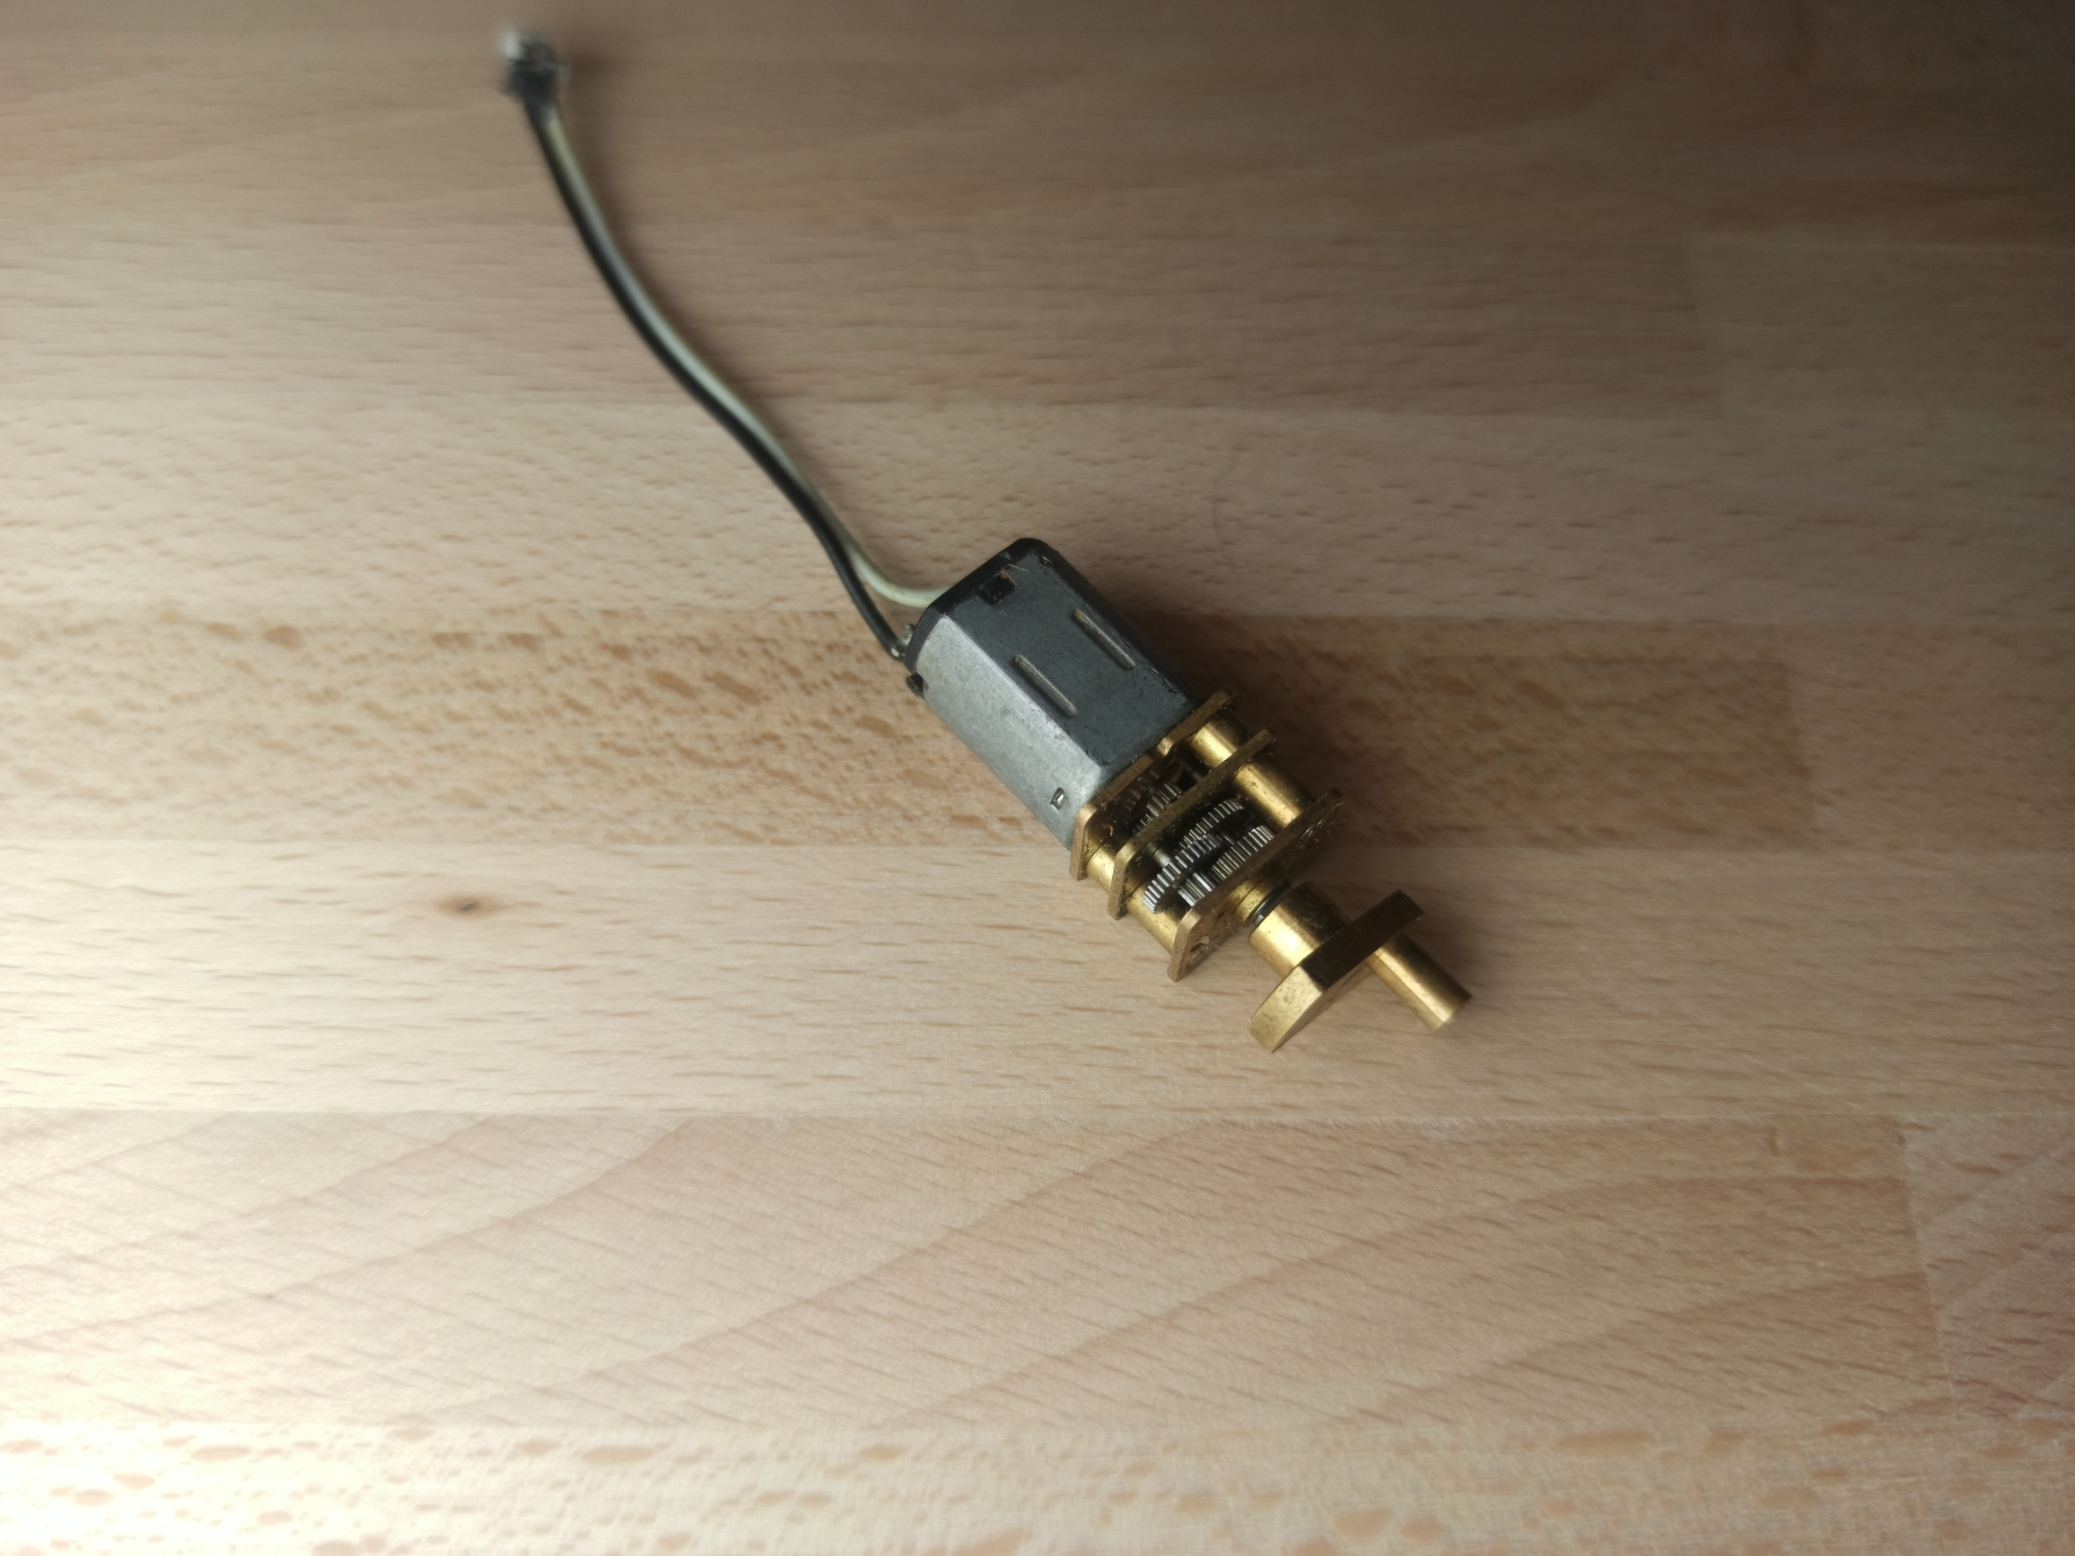
\includegraphics[width=160]{kapitoly/obrazky/E3/motory/hodinovyStrojek.jpg}
    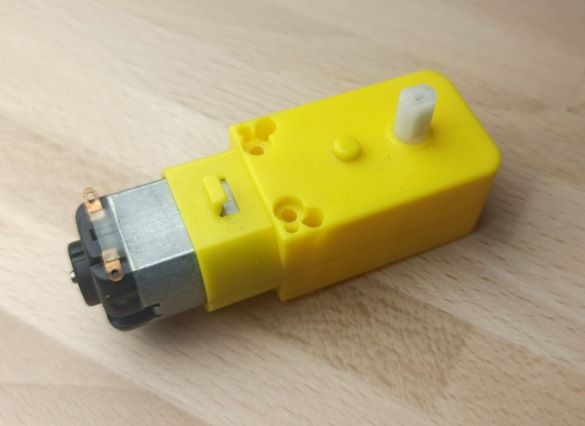
\includegraphics[width=160]{kapitoly/obrazky/E3/motory/zluty_motor.jpg}
    \label{fig:M1}
\end{figure}

\begin{figure}[htbp]
    \centering
    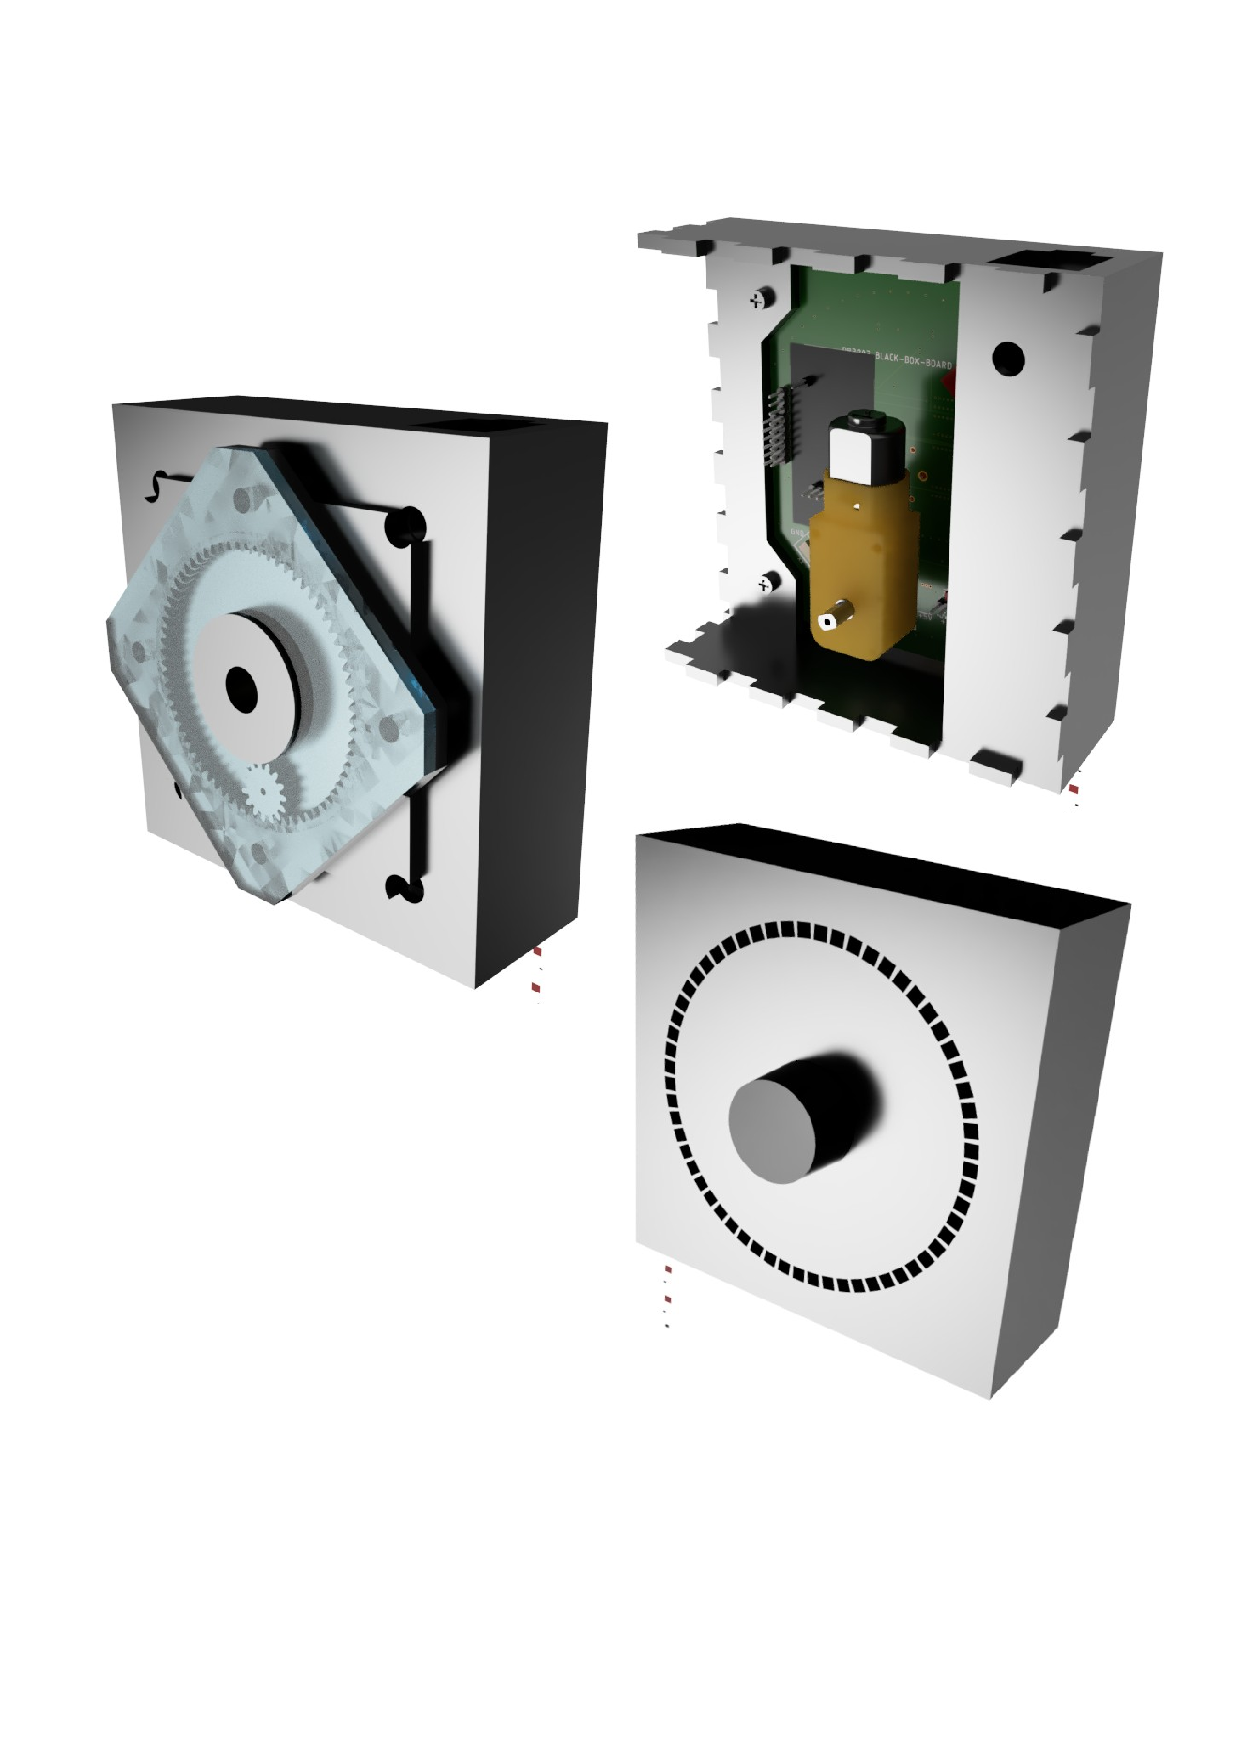
\includegraphics[width=\textwidth]{kapitoly/obrazky/E3/rendery.pdf}
    \label{fig:M1}
\end{figure}

Přes velké množství funkcí jsem, kvůli několika věcem ale opět koncept přepracoval. Hlavním důvodem změn bylo náročné uložení rotační západky, 
které vyžadovalo ozubený věnec a několik dalších tisknutých dílů.

\newpage
\section{Čtvrtá verze}
\label{E4-vivoj}

\subsection*{Rozšíření elektroniky}

Čtvrtá verze byla co se elektroniky týče přímým pokračováním předchozí verze (viz kapitola \ref{E3-vyvoj}), kterou dále rozšiřuje.

Trezor získal oproti minulé verzi schopnost komunikace pomocí IR z důvodu identifikace růz\-ných dveří, dále získal magnetický enkodér, pro možnost snaz\-ší\-ho ovládání
motoru zámku. 
Další inovací byl programovací systém s~USB-C, na místo USB-micro jako dřív. Nový programátor má možnost úplně si odpojit napáje\-ní, a~to~v~rámci šetření 
energie, když trezor programátor nevyužívá. 
Zároveň umožňuje zákaz přeprogramování.

Podstatnou změnou také bylo rozdělení elektroniky do dvou různých desek, protože na jedné by nebyl dostatek místa. Jedna deska \obr{fig:E4-sch_next-board}, \obr{fig:E4-LedDeska}
tak obsahuje kruh LED \parencite{WS2812} a čip LDC1614 \parencite{LDC1614} nebo LDC1314 se čtyřmi cívkami, které měří vzdálenost tlakové desky. Na druhé desce
je vše ostatní, tedy procesor \parencite{ESP32}, akcelerometr a
gyroskop \parencite{bmx055}, \parencite{mpu6050}, magnetický kompas \parencite{bmx055}, \parencite{qmc5883}, RTC\footnote{Real Time Clock, hodiny reálného času} \parencite{m41t62}, 
barometr \parencite{spl06}, IR vysílač \parencite{ir19-21c/tr8} a přijímač \parencite{irm-h936}, magnetický enkodér \parencite{mh253}, \parencite{ss360nt}, programátor \parencite{cp2102},
řešení napájení, řízení motoru a nabíječka \parencite{se9017}. 

\subsection*{Princip zamykání}

Na trezoru se dále změnily princip zamykání a ovládání. 

Důvodem změn bylo náročné uložení rotační západky, 
které vyžadovalo ozubený věnec a několik dalších tisknutých dílů.
Z tohoto důvodu také již není možné použít tělo mechanického trezoru pro elektronickou variantu.

Zamykání je založeno na mechanizmu bajonetu a zamčení je zajištěno západ\-kou, která zabraňuje zpětnému otočení.
Západka je ovládána motorem, který otáčí magnetem a přitahuje nebo odpuzuje magnet na západce. Důvodem pro magnetické ovládání
byla možnost západku ovládat i přes pevnou stěnu, a~také pružné spojení, které takto vznikne, takže se trezor například dá zavřít, i~když
je už zamčen (když například dveře nejsou dovřeny).

\begin{figure}[htbp]
    \centering
    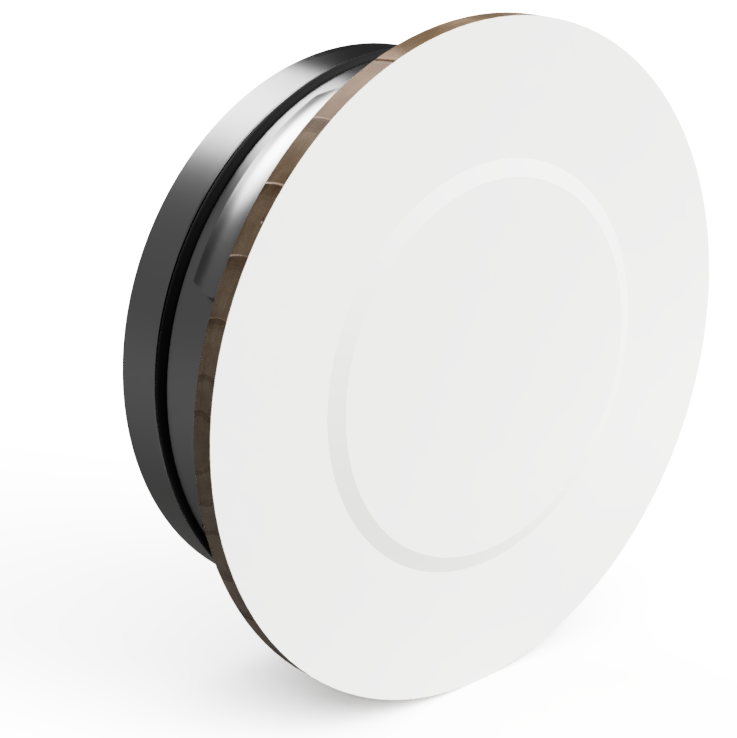
\includegraphics[width=170pt]{kapitoly/obrazky/E4/predni_render.png}
    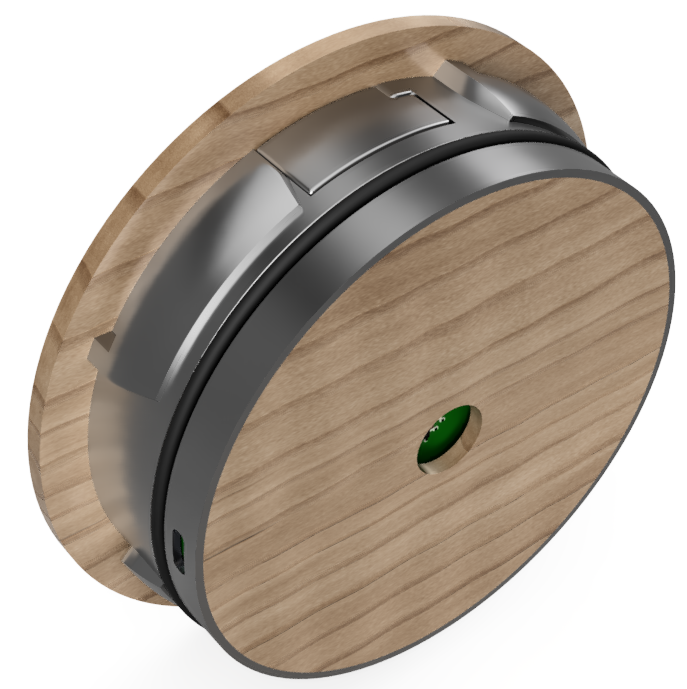
\includegraphics[width=170pt]{kapitoly/obrazky/E4/zadni_render.png}
    \caption{Rendery dveří trezoru E4 -- vlevo přední pohled, vpravo zadní pohled \centering}
    \label{fig:E4-render}
\end{figure}

\subsection*{Ovládání}
Předchozí varianty měly jako hlavní ovládací prvek enkodér s tlačítkem, ten jsem v nynější variantě odstranil, aby přední stěna neměla tak velký 
výstupek. Proto jsem tento prvek nahradil indukční tlakovou deskou \ref{E4-tlakovka}, která vyplnila vnitřek kruhu ledek \ref{WS2812}. 
Zbytek ovládání víceméně přetrval, jen kvůli nedostatku času a~pandemií způsobenému nedostatku součástek, trezor přišel o GPS.\footnote{Deska má ale stále možnost připojení GPS pomocí konektoru.}
Na druhou stranu ale získal barometr s rozlišením schopným detekovat změnu výšky o půl metru.

\subsection*{Napájení}
Předchozím verzím sloužila jako napájení powerbanka. Ta však kladla poměrné velké omezení, dokázala poskytnout proud pouze jednoho ampéru, a proto 
jsem jí nahradil vlastním zdrojem, dvěma bateriemi 18650. 
To samozřejmě znamenalo nutnost vlastního řešení stabilizace napětí, díky čemuž trezor dostal stepup FP6276 \parencite{fp6276a}, \obr{fig:E4-step-up}, 
který spíná napětí z 3,5~V až 4,2~V na 5~V, a původně stepdown, později lineární stabilizátor \obr{fig:E4-stabilizator}, který poskytuje 3,3~V. 

Trezor také dostal vlastní nabíječku, aby pro nabíjení baterií stačilo připojit kabel, stejně jako třeba u mobilu.


\chapter{Vývoj mechanického trezoru}
\label{M-vyvoj}

\section{První verze}
\label{M1-vyvoj}

\begin{wrapfigure}{R}[20mm]{0.4\textwidth}
    \centering
    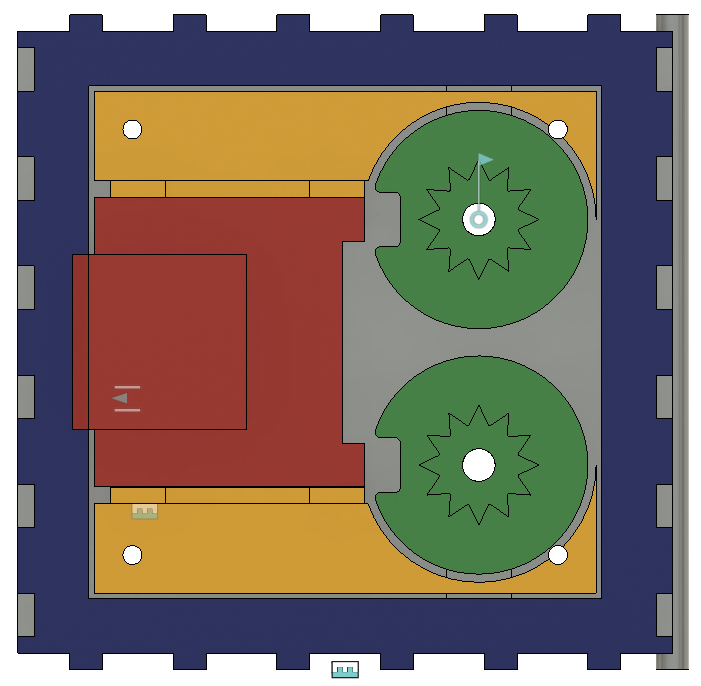
\includegraphics[width=0.4\textwidth]{kapitoly/obrazky/M1/mechanizmus.png}
    \caption{Zelená barva značí kódovací kola, červená západku, modrá pevnou část trezoru a žluté díly distanci \centering}
    \label{fig:M1-mechanizmus}
\end{wrapfigure}
První čistě mechanická varianta, označovaná jako M1, vznikla začátkem srpna 2019, brzy po první  elektronické variantě.
Měla stále poměrně klasický vzhled trezoru -- zamykatelná skříňka se dvěma  kódovacími koly, která ovládala možnost pohybu jednoduché západky.

Tato verze byla také určená jako základ pro plánovaný upgrade na další elektronickou
variantu. Na podobné vylepšení mělo stačit odstranění kódo\-va\-cích kol a přidělání elektronické části. Toto sice fungovalo obstojně, zároveň 
i~jako motivace, ale kvůli pozdější změně konceptu mechanizmu uzavírání trezoru\footnote{místo rotační západky mechanizmus bajonetu -- viz kapitola %todo
} tento nápad padl.

Tato varianta se také ukázala jako nevhodná\footnote{kvůli přílišné náročnosti na přesnost sesazení} pro stavbu s malými dětmi, 
pro které byla určena jakožto předstupeň k variantě elektronické (která vyžaduje i~znalosti programování nebo alespoň ochotu se jej  učit).

\newpage
\section{Druhá verze}

Druhá mechanická varianta má oproti první verzi daleko vetší počet možných kombinací.
Ovládá se pěti koly. Čtyři z nich nastavují heslo a páté otáčí s~rotační západkou, která drží dveře na svém místě.

Tato varianta taky přichází s možností dveře úplně oddělit od skříně trezoru. To by při využití jako trezor, který
má za úkol jen ochraňovat svůj obsah, sice nepřinášelo žádný velký užitek, ale při mém využití, spíše jako herní 
prvek než trezor, to může být užitečné.

\begin{figure}[htbp]
    \centering
    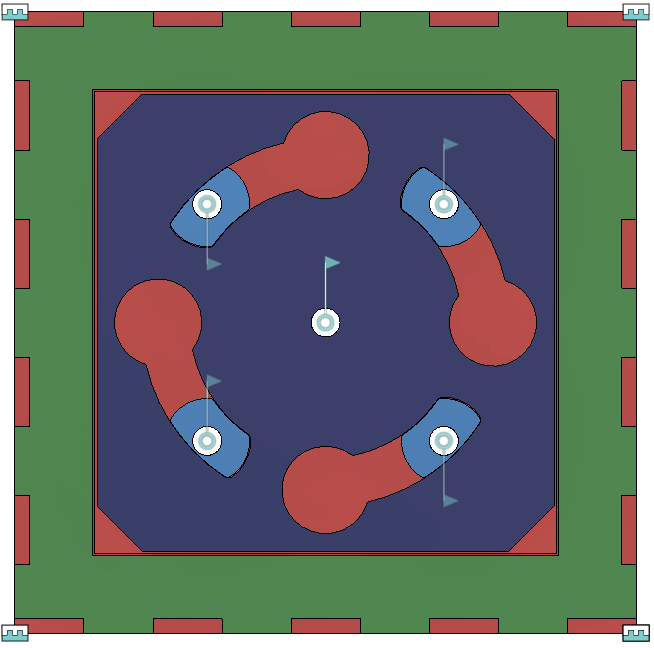
\includegraphics[width=150pt]{kapitoly/obrazky/M2/mechanizmus_odemcen.png}
    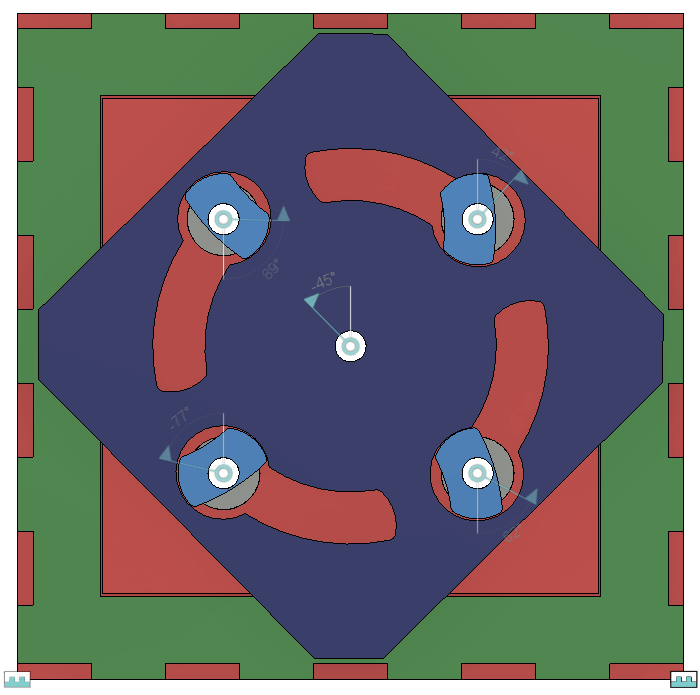
\includegraphics[width=150pt]{kapitoly/obrazky/M2/mechanizmus_zamceno.png}
    \caption{zamykací mechanizmus varianty M2}
    \label{fig:M2-mechanizmus}
\end{figure}

\begin{figure}[htbp]
    \centering
    \includegraphics[width=\textwidth]{kapitoly/obrazky/M2/predni_render.PNG}
    \caption{render varianty M2}
    \label{fig:M1.0}
\end{figure}


\newpage
\section{Třetí verze}

\begin{figure}[htbp]
    \centering
    \includegraphics[width=70pt]{kapitoly/obrazky/M3/predni_render.png}
    \caption{Render varianty M3}
    \label{fig:M3-render}
\end{figure}

Dnešní mechanická varianta je téměř stejná jako druhá verze, rozdíl je jen v~uložení kol, které kolem hřídelů získalo distanční kroužky, které
zjednodušují lepení. 

\begin{figure}[h]
    \centering
    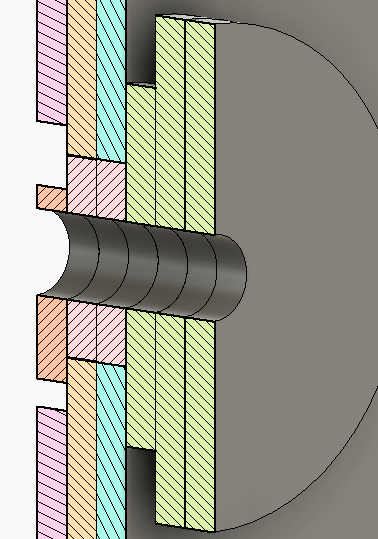
\includegraphics[width=0.4\textwidth]{kapitoly/obrazky/M3/rez.png}
    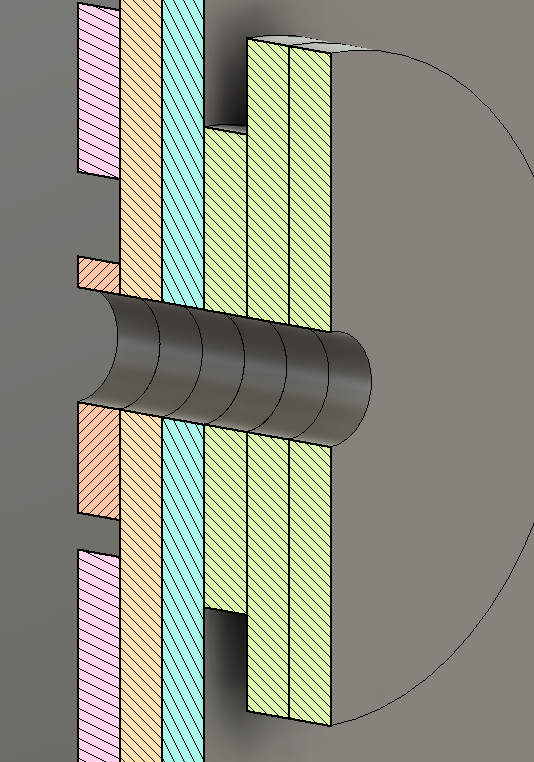
\includegraphics[width=0.4\textwidth]{kapitoly/obrazky/M2/rez.png}
    \caption{Řez kódovacím kolem trezoru M2 vlevo a řez kódovacím kolem trezoru M3 vpravo \centering}
    \label{fig:M3-rez-kolem}
\end{figure}

\newpage

\chapter{Mechanický trezor} 
\label{M3}

\label{M3}
Vedle elektronické varianty jsem navrhl i~variantu čistě mechanickou, abych měl jednodušší 
a~levnější trezor pro mladší účastníky táborů a~jiných akcí. 
Mechanická varianta měla opět několik vývojových verzí. Jednotlivé verze a~jejich vlastnosti 
jsou popsány v~samostatné příloze. V~přílohách jsou také přiloženy výkresy poslední mechanické verze. 
Pro představu je v~příloze tohoto souboru uveden obrázek poslední mechanické verze \ref{fig:M2-render}. 

\begin{figure}[h]
	\centering
    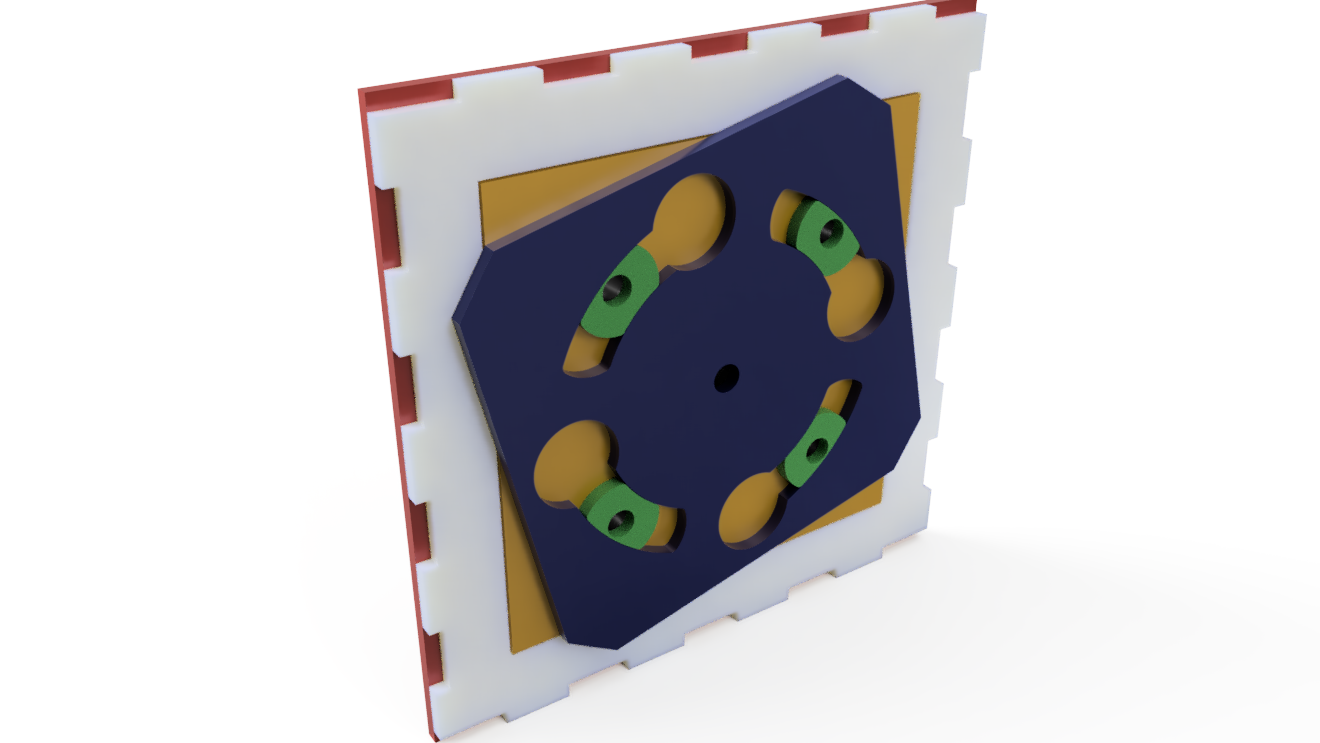
\includegraphics[width=\textwidth]{kapitoly/obrazky/M3/SOC_render.png}
    \caption{Vzhled mechanizmu zamykání u~mechanické verze}
    \label{fig:M3}
\end{figure}

\section{Popis jednotlivých součástek a důvody konkrétního tvaru}

\begin{wrapfigure}{R}[0.2\textwidth]{0.7\textwidth}
    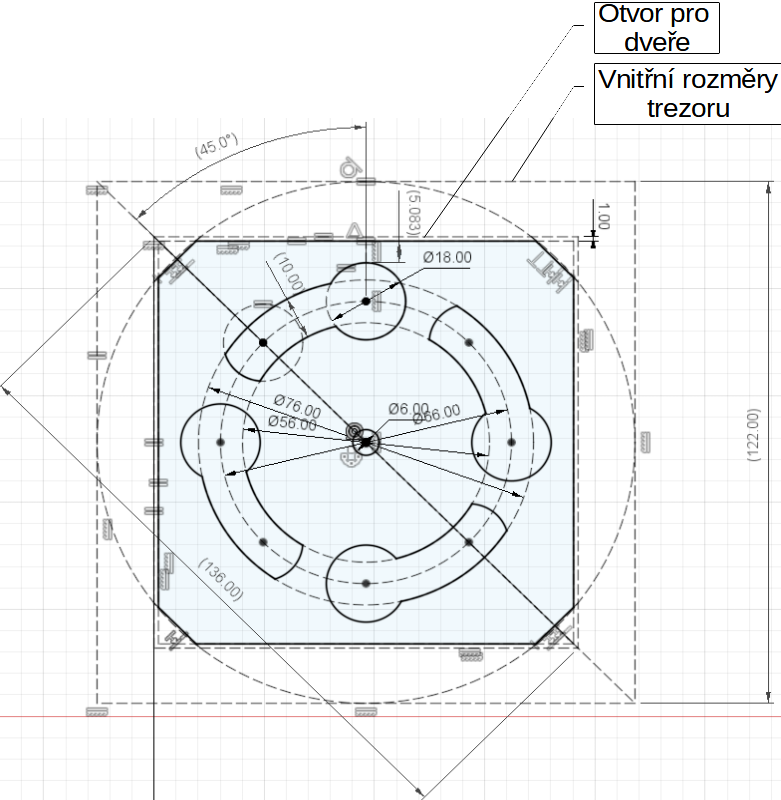
\includegraphics[width=0.7\textwidth]{kapitoly/obrazky/M3/geometrie_zapadky.png}
    \caption{náčrt} %todo čeho náčrt? 
    \label{fig:M3-geometrie-zapadky}
\end{wrapfigure} %todo zvážil bych obrázek centrovaný a obtékaný pouze nahoře a dole 

\subsection*{Geometrie západky}
Trezor má tvar krychle a~délku hrany má 128~mm, násobek šestnácti jsem zvolil kvůli jednoduché návaznosti na dřívka, %todo přidáme pár vět o dřívkách 
 dřevěná dřívka s obdélníkovým průřezem 3x16~mm nebo 2x16~mm. 
Protože je trezor vyroben z překližky o síle 4~mm, jsou jeho vnitřní rozměry o 4~mm na každé straně menší (takže 122~mm). 

%todo tady asi chybí další tvary? 
%\section{Odolnost proti násilnému vniknutí}
Základní druhý namáhání, kterým musí trezor odolat, jsou

\begin{itemize}
    \item snaha o vytržení dveří 
    \item snaha o odemčení bez znalosti hesla
\end{itemize}

\paragraph{Vytržení dveří}
Jedním ze způsobů~namáhání~mechanizmu~je~vytržení~dveří~z~trezoru.

\subsection{Západka}

\begin{figure}[htbp]
    \centering
    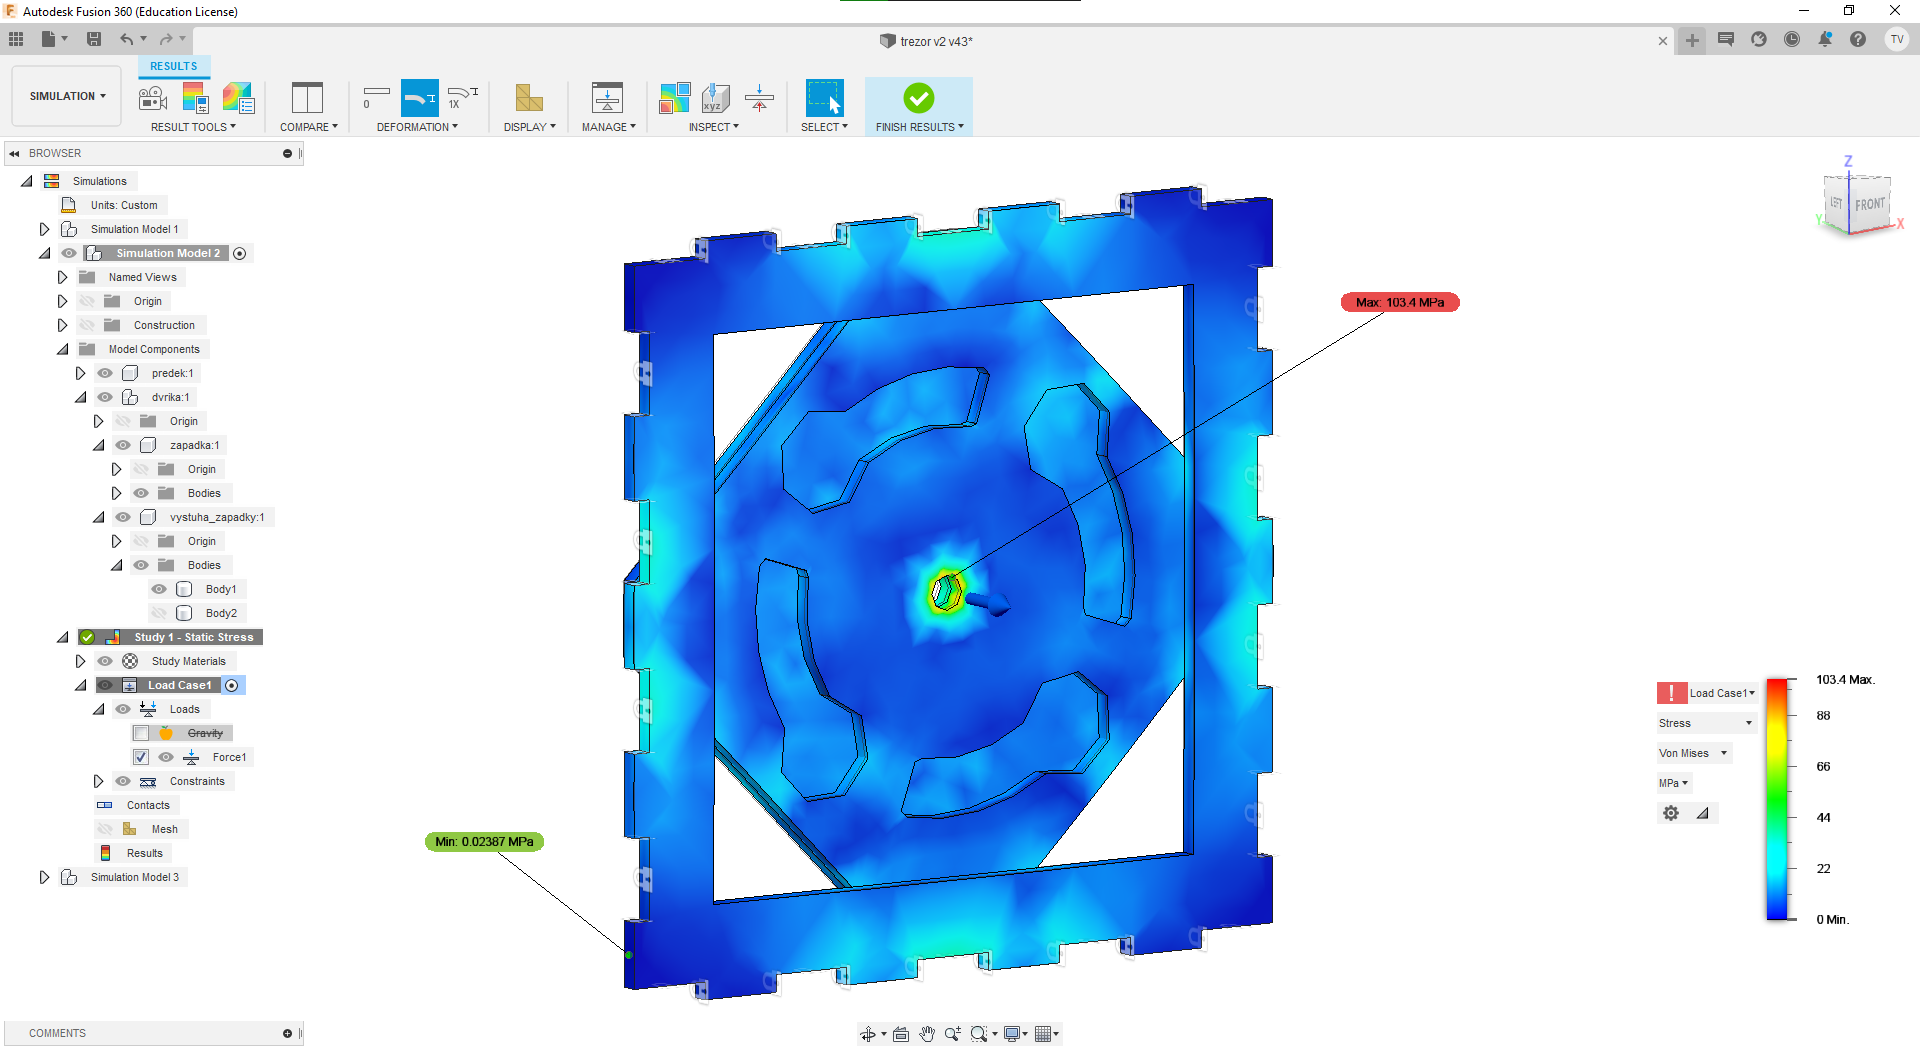
\includegraphics[width=\textwidth]{kapitoly/obrazky/M3/simulace/odolnost_proti_vytrzeni_4kN.png}
    \caption{Simulace pokusu o vytržení dveří silou 4 000 N}
    \label{fig:M3-simulace-vytrzeni}
\end{figure}
Ke kompletní simulaci se můžete dostat \href{https://myhub.autodesk360.com/ue2d7aa41/g/shares/SH56a43QTfd62c1cd96843f1e03a0eb48053?viewState=NoIgbgDAdAjCA0IDeAdEAXAngBwKZoC40BlASwFsBXAGwEN1SB7AOzXjVoGdPd1C0ARjABsATlEQItALQBjcbmkAWCMIjSBuWgA5lAM22ilAVgAmMAOyy9\%2BBGkYCAVrlnoAkqcIBmAL4gAukA}{zde}
po kliknutí na \uv{Simulation} a~\uv{Simulation Model 2}. V tabulce napravo se pak můžete přepínat mezi barevným zobrazení několika veličin.

\newpage

\subsection{Kolík}
Při pokusu o vytržení je celá síla přenášena kolíkem.

\begin{table}[h]
    \centering
    \resizebox{0.4\textwidth}{!}{%
    \begin{tabular}{l|l}
    $ \sigma $  & napětí v materiálu    \\
    $ D $       & průměr kolíku         \\
    $ F $       & působící síla         \\
    $ S $       & plocha průřezu kolíku \\
    \end{tabular}%
    }
    \caption{Tabulka použitých symbolu pro napětí v kolíku v tahu}
    \label{tab:M3_symboly_kolik}
\end{table}

 $ \sigma $     

 $ \sigma_{max} = 132  $ MPa    ( \href{https://is.mendelu.cz/eknihovna/opory/zobraz_cast.pl?fit_w=1;cast=9190}{dubové dřevo ve směru vláken při vlhkosti 12 \% }) % strana 22 tabulka 2 -> https://www.vutbr.cz/www_base/zav_prace_soubor_verejne.php?file_id=66237

$D = 6$ mm %todo popis všech veličin

 \(\sigma_{max} = F/S \Rightarrow F = \sigma_{max} \cdot S = 132 \cdot (\pi \cdot D^2/4) = 3 732,21 \) N  z toho a ze simulace vyplývá že kolík je při namáhání nejslabším členem.

\paragraph{Otevření bez odemčení}
Dalším způsobem namáhání může být snaha otočit západkou pez zadání správného hesla.

\subparagraph{Západka}

\begin{figure}[htbp]
    \centering
    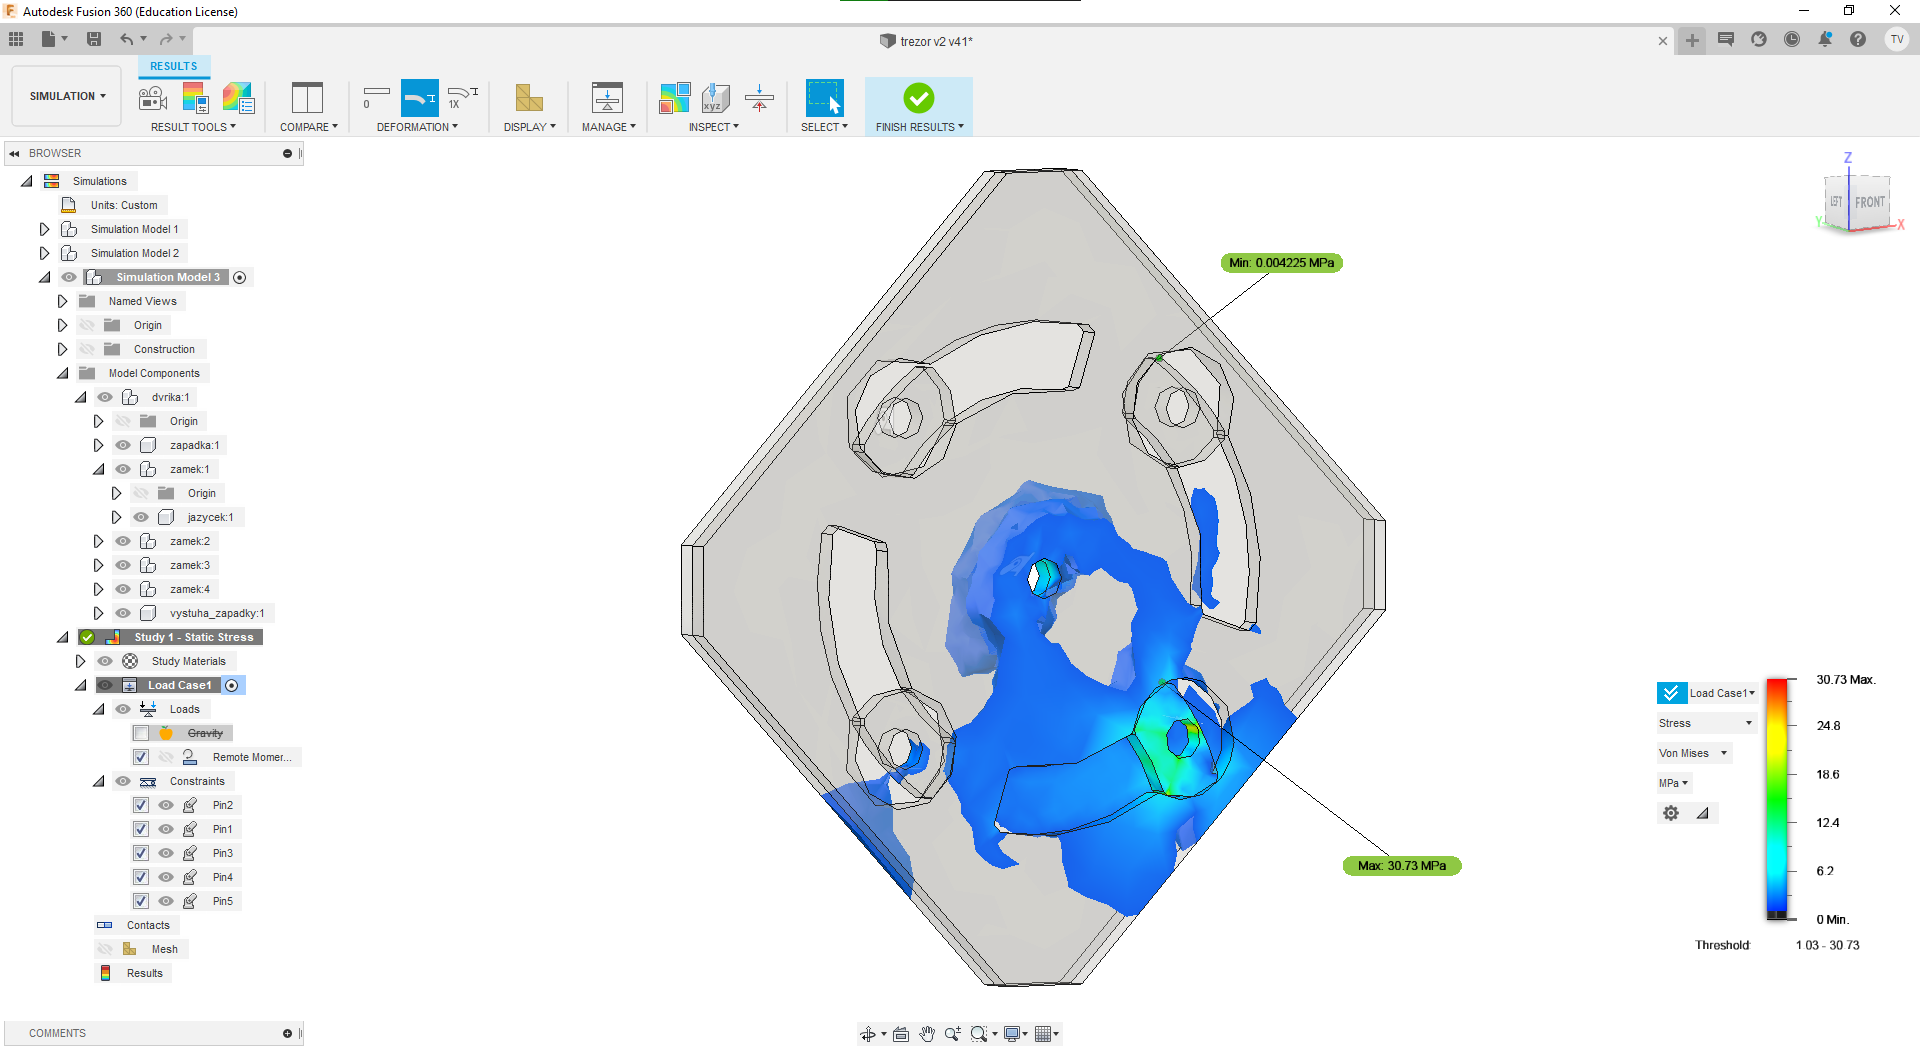
\includegraphics[width=\textwidth]{kapitoly/obrazky/M3/simulace/odolnost_proti_nasilnemu_odemceni_10Nm.png}
    \caption{Simulace pokusu o otevření bez předchozího odemčení při kroutícím momentu 10 000 Nmm, zobrazeno jen napětí nad 1 MPa}
    \label{fig:M3-simulace-vytrzeni}
\end{figure}

Ke kompletní simulaci se můžete dostat \href{https://myhub.autodesk360.com/ue2d7aa41/g/shares/SH56a43QTfd62c1cd96843f1e03a0eb48053?viewState=NoIgbgDAdAjCA0IDeAdEAXAngBwKZoC40BlASwFsBXAGwEN1SB7AOzXjVoGdPd1C0ARjABsATlEQItALQBjcbmkAWCMIjSBuWgA5lAM22ilAVgAmMAOyy9\%2BBGkYCAVrlnoAkqcIBmAL4gAukA}{zde}
po kliknutí na \uv{Simulation} a~\uv{Simulation Model 3}. V tabulce napravo se pak můžete přepínat mezi barevným zobrazení několika veličin.

\subparagraph{Kolík}
Kroutící moment, který je dřevěný kolík o průměru D = 6~mm schopen přenést. 

\begin{table}[h]
    \centering
    \resizebox{0.4\textwidth}{!}{%
    \begin{tabular}{l|l}
    $ \tau $    & napětí v materiálu při krutu      \\
    $ D    $    & průměr kolíku                     \\
    $ M_k  $    & kroutící moment                   \\
    $ W_k  $    & průřezový modul v krutu           \\
    \end{tabular}%
    }
    \caption{Tabulka použitých symbolu pro napětí v kolíku v tahu}
    \label{tab:M3_symboly_kolik}
\end{table}

$ \tau_{max} = 52,3 $ MPa (\href{https://is.mendelu.cz/eknihovna/opory/zobraz_cast.pl?fit_w=1;cast=9190}{dubové dřevo ve směru vláken při vlhkosti 12 \% })

$ \tau_{max} = \frac{M_k}{W_k} \Rightarrow M_k = \tau_{max} \cdot W_k = \tau _d \cdot \frac{\pi \cdot D^3}{16} $

$ M_k = 52,3 \cdot \frac{\pi \cdot 6^3}{16} = 2 218,16 $ N*mm. Z výpočtu a ze simulace plyne, že kolík je při namáhání v krutu nejslabším místem. Pro zvýšení odolnosti by proto bylo 
potřeba zvětšit kolík nebo změnit materiál.

\newpage
\chapter{Elektronický trezor}
\label{E4}

\section{Přehled}

Dnešní verze elektronického trezoru se zamyká pomocí mechanizmu bajonetu a magneticky řízené zpětné západky. 

Elektronika je vybavena čipem ESP32 \parencite{ESP32}, \parencite{ESP32-WROVER-B},
který obsahuje dva procesory Xtensa LX6, WiFi a bluetooth. Dále je trezor vybaven čipem BMX055 \parencite{bmx055} nebo dvojicí čipů MPU6050 \parencite{mpu6050} 
a QMC5883 \parencite{qmc5883} které poskytují 
gyroskop, akcelerometr a magnetický kompas. Dále je zde SPL06 \parencite{spl06}, barometr s rozlišením 0,06~hPa, což umožňuje rozeznat změnu nadmořské výšky 
o polovinu metru. Další systém trezoru je možnost IR komunikace, která je zde pro možnost jednoznačné identifikace dveří, ale pochopitelně může 
sloužit i pro jiný účel. Deska je také vybavena RTC \footnote{Real Time Clock, hodiny reálného času} a má vlastní programátor pro usnadnění programování. Vedle ESP32 je zde asi 
nejvýznamnějším čipem LDC1614 \parencite{LDC1614}, případně LDC1314, který umožňuje funkci tlakové plochy (viz kapitoly \ref{E4-tlakovka} \ref{E4-mech_tlakovky}).

%todo doplnit popis a využití a možnosti tlakové desky 

\begin{table}[h]
    \centering
    \resizebox{\textwidth}{!}{%
    \begin{tabular}{@{}lll@{}}                                                                                 \\ \midrule
    \textbf{ESP32}              & dva procesory Xtensa LX6, WiFi a bluetooth    &                                                                           \\
    \textbf{BMX055}             & gyroskop, akcelerometr, magnetický kompas     & možno nahradit dvojicí čipů MPU6050 a QMC5883                             \\
    \textbf{SPL06}              & barometr                                      & rozlišení až 0,06hPa což umožňuje rozeznat změnu nadmořské výšky o 0,5m   \\
    \textbf{IRM-H936 a IR led}  & IR komunikace                                 &                                                                           \\
    \textbf{LDC1614}            & snímání tlakové desky                         & počítá se s možnou záměnou za LDC1314                                     \\
    \textbf{CP2102}             & programátor                                   & s hardwarově zajištěným odpojováním napájení, pokud není využíván          \\ \bottomrule
    \end{tabular}%
    }
    \caption{Shrnutí elektronického vybavení}
    \label{tab:COMPARATION}
\end{table}

\newpage
\section{Mechanika tlakové desky}
\label{E4-mech_tlakovky}

Indukčně snímaná tlaková deska funguje díky čtyřem cívkám na desce ploš\-ných spojů, které mění svojí indukčnost podle vzdálenosti snímané desky, terčíku.
Z tohoto důvodu se terčík při používání naklání, čímž zároveň mění svojí vzdálenost od jednotlivých cívek. Z toho také plyne nutnost uložit terčík
částečně volně. Terčík je proto od snímací desky oddělen pružnou vložkou, která je zároveň předepnuta pomocí nažehlovací fólie, která kryje přední 
stranu dveří a spojuje terčík s čelní krycí deskou. Díky nažehlovací fólii je také přední část dveří voděodolná.

\begin{figure}[h]
    \centering
    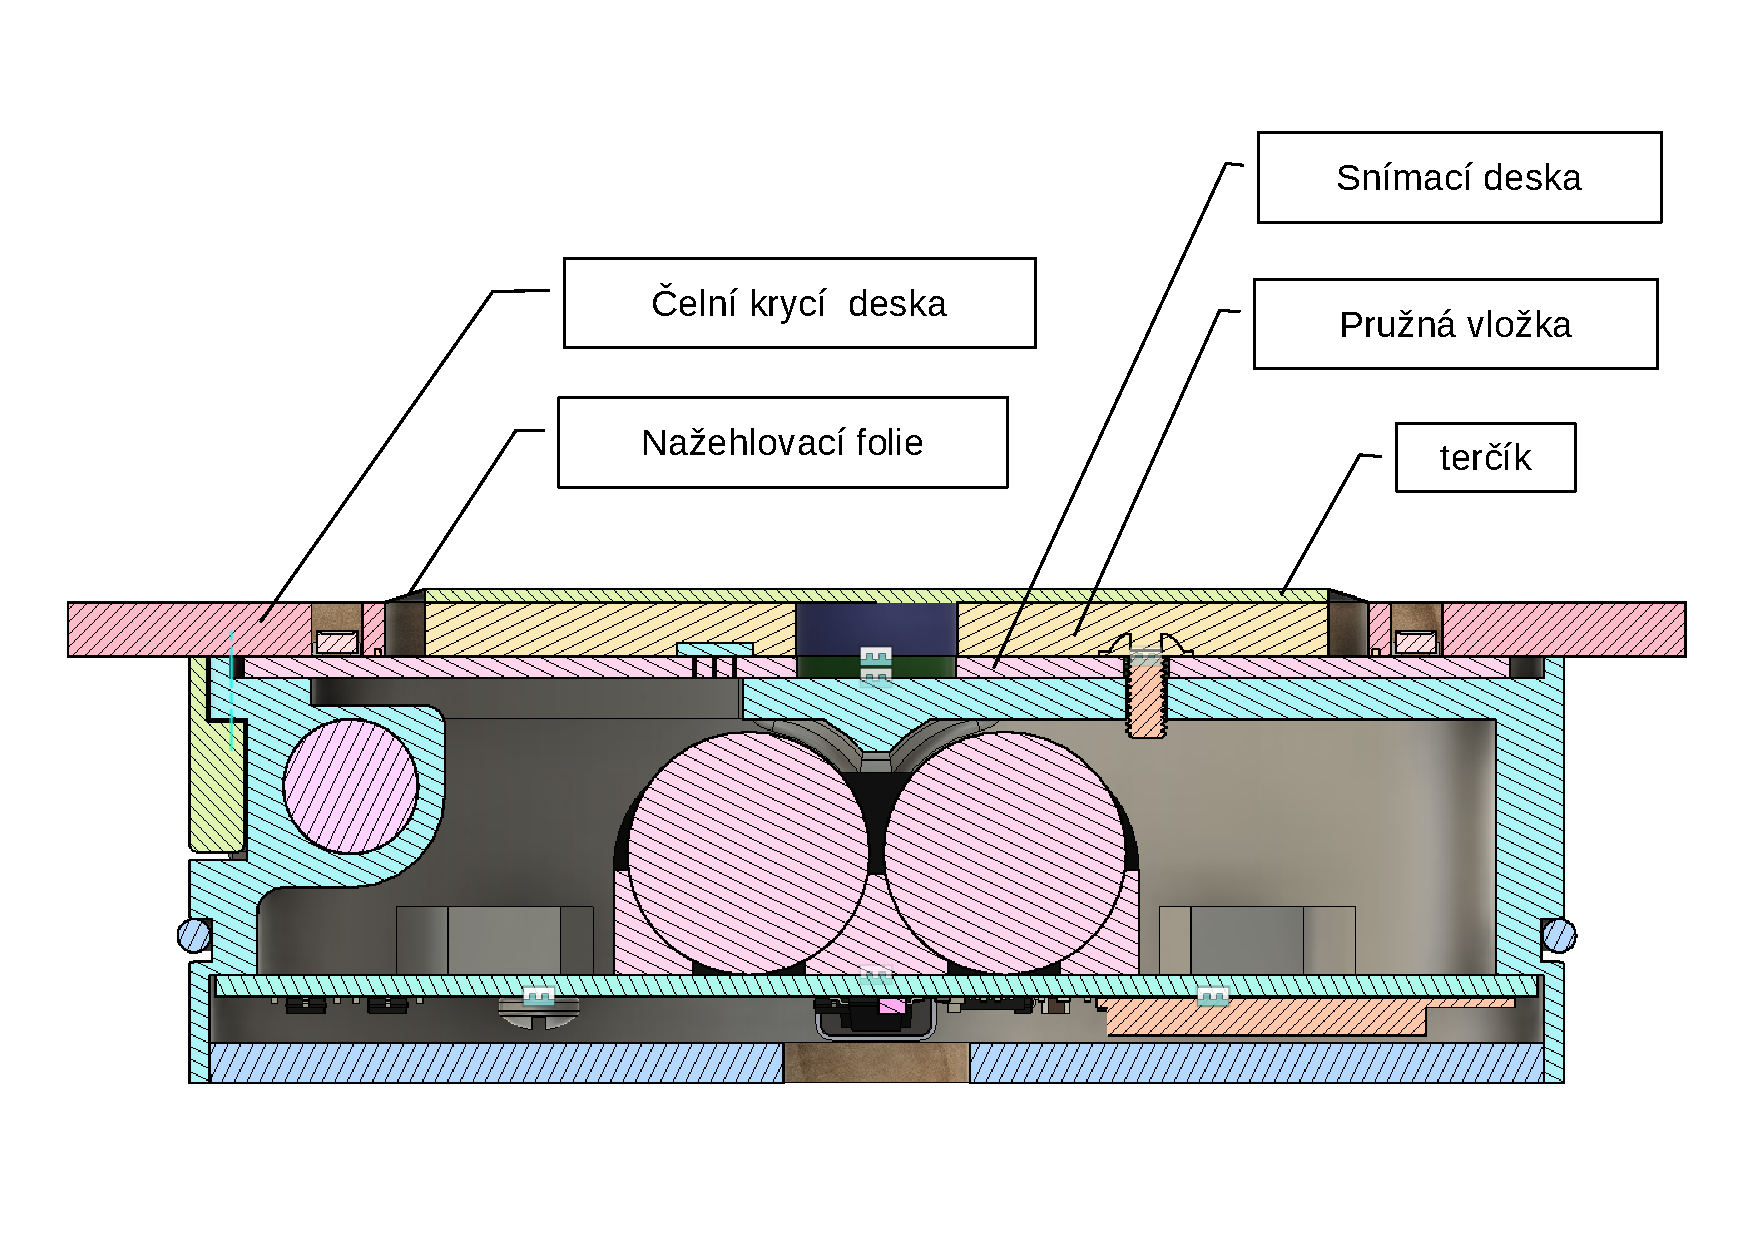
\includegraphics[width=\textwidth]{kapitoly/obrazky/E4/machanika_tlakove_desky/rez_po_ose.pdf}
    \caption{Řez varianty E4}
    \label{fig:E4-rez}
\end{figure}

\newpage

Díky zkušenostem z jiného podobného projektu jsem zjistil, že ovládací prvek by měl být co možná největší. 
Zároveň by měl odolat i poměrně silným ranám, které děti v zápalu hry zařízení uštědřují.
Tlaková deska tedy počítá s možností působení síly o velikosti až 500~N, což samozřejmě zároveň znamená, že tělo dveří tomuto zatížení musí odolat.
Vzhledem k tomu, že nemám možnost vyrobit tělo z kovu a jsem odkázán na 3D tisk a laserovou řezačku, a zároveň chci mít dveře co možná nejmenší,
musel jsem napočítat kritické části těla tak, aby odolaly a zároveň nebyly příliš mohutné. Z tohoto důvodu jsem v programu Fusion 360, ve kterém jsem trezor vyvíjel,
dělal simulaci, kterou k práci přikládám na obrázcích \obr{fig:E4-simulace_tela} a \obr{fig:E4-simulace_tlakovky}.

Jako materiál těla jsem v první fázi zvolil standardní fotopolymer pro tiskárny typu SLA, s pevností v tahu 46 až 67 MPa.
V budoucnu bych ale chtěl tělo odlévat z nějakého houževnatého polyuretanu, aby se zlevnila výroba a zároveň stoupla odolnost.
\section{Zpětná západka}

Zpětnou západkou pohybuje motor pomocí magnetu. Pro zajištění vodě\-o\-dol\-nos\-ti je motor od západky oddělen stěnou, což je také jeden z~důvodů použití magne\-tic\-ké\-ho spojení.

\begin{figure}[h]
    \centering
    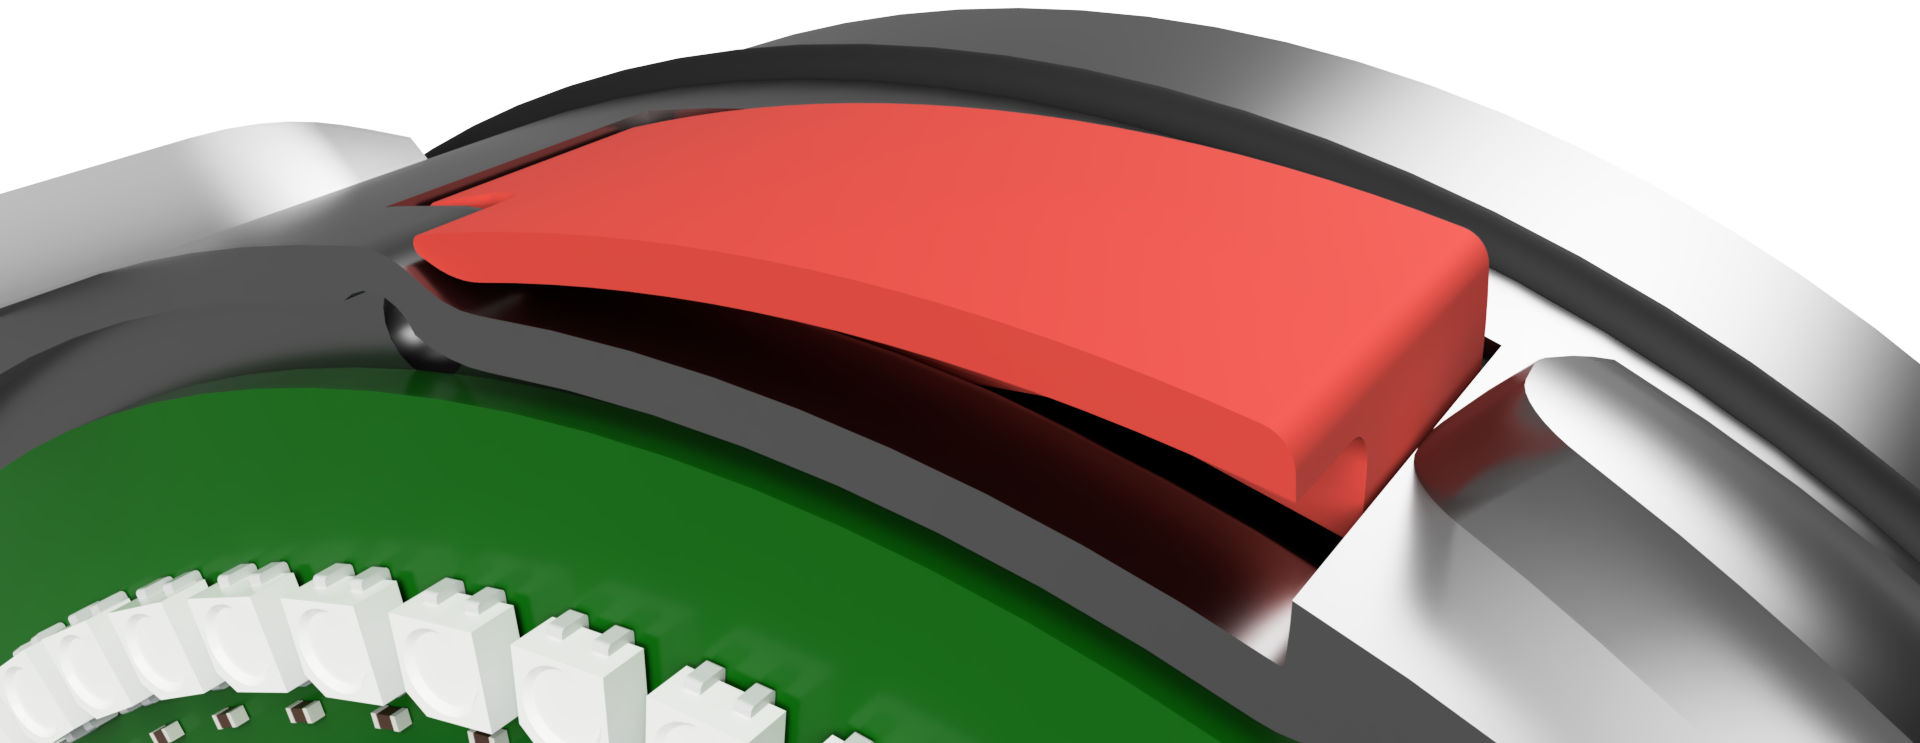
\includegraphics[width=\textwidth]{kapitoly/obrazky/E4/zapadka/render.png}
    \caption{Render západky}

    \label{fig:E4-zapadka}
\end{figure}

\paragraph{Sklon čela}
\addcontentsline{toc}{paragraph}{Sklon čela}

Aby při zamčení západka doléhala na otvor trezoru a zároveň neměla příliš velkou vůli, je potřebné správně navrhnout tvar západky.
Jednou z možností je navrhnout čelní plochu\footnote{Plocha, která je při zamčení v kontaktu se dveřním otvorem.} jako část válcové plochy. 
Sice teoreticky není problém na FDM tiskárně\footnote{typ 3D tiskárny tisknoucí z tiskové struny} vytisknout západku s takovou plochou čela,  %todo nechápu <- lepší?
a na laseru vypálit vhodný protikus\footnote{Stejná plocha totiž musí být i v otvoru, do kterého se dveře umístí.},
ale výsledná plocha je hlavně u tisku nevzhledná a je třeba jí obrousit do požadovaného vzhledu. Obrousit válcovou plochu je však náročnější než plochu rovnou, zvlášť v otvoru trezoru, 
a je tedy pro mě výhodnější navrhnout tuto plochu jako rovinu a jen ji správně sklonit. Špatně navržený sklon by se projevil buď přílišnou vůlí, 
což by znamenalo, že by se dveře v trezoru viklaly a nebo by západka nebyla samosvorná, což by se projevilo možností trezor otevřít vetší silou 
i~bez jeho odemčení.

\begin{figure}[htbp]
    \centering
    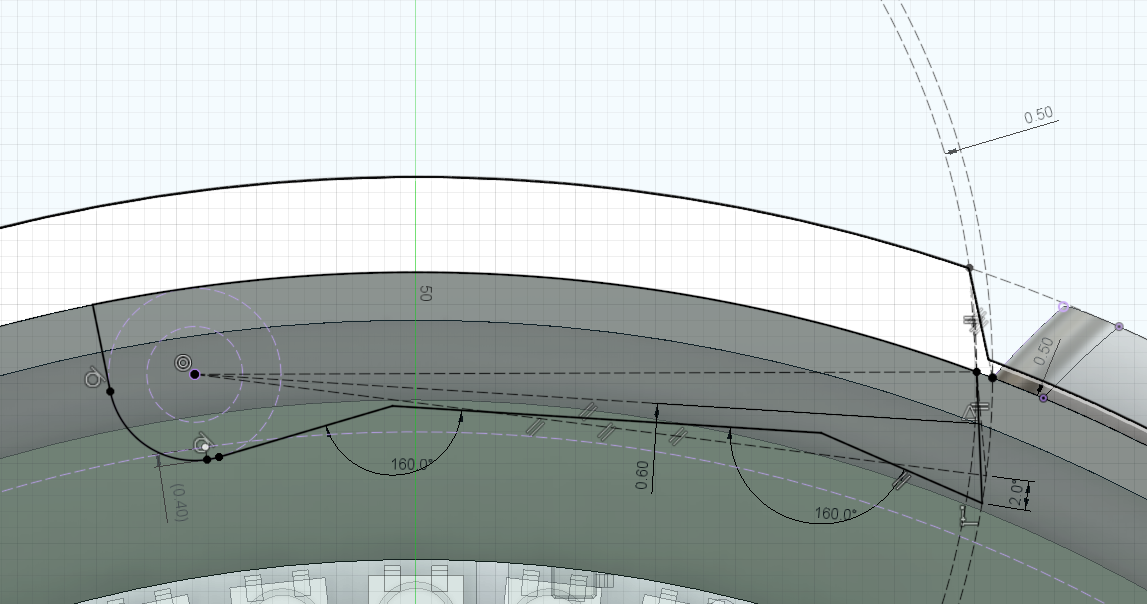
\includegraphics[width=\textwidth]{kapitoly/obrazky/E4/zapadka/uhel_cela.png}
    \caption{Geometrie západky}
    \label{fig:E4-uhel_cela_zapadky}
\end{figure}


\paragraph{Západka v průběhu vývoje}
\addcontentsline{toc}{paragraph}{západka v průběhu vývoje}

Západka se ve vývoji pochopitelně objevila společně s bajonetem, ale v první verzi byla jen částí těla dveří a teprve v~dalších verzích se stala
samostatnou součástkou. První tělo využívající bajonet jsem tiskl na FDM tiskárně z plastu PLA a západka byla jen jeho pružnou částí. Toto řešení sice 
z počátku fungovalo a mělo výhodu jednoduší výroby, ale PLA po několika měsících začalo ztrácet pružnost a západka se už nepohybovala v celém rozsahu.
Toto jsem z počátku chtěl řešit samostatnou západkou ve spojení s tažnou pružinou. Pružiny však nebyla třeba a naprosto stačí magnet na motoru a v západce.
Západka proto zůstala v teto podobě a~jen se přidala mechanická přepážka kvůli voděodolnosti. 

Západka je také v neposlední řadě navržena tak, aby odolala pokusu o vylomení za působení kroutícího momentu o velikosti až 5000 N$\cdot$mm, výsledky simulace najdete 
na obrázku \obr{fig:E4-simulace_zapadky}.


{\tiny }\section{Úkosy}

    Aby bylo jednodušší při zavírání dveře správně natočit, mají zarážky na vnitřní straně velké úkosy, které tak zvětšují na vnitřní straně 
vůli a při zasouvání navedou dveře do správné pozice.


\begin{figure}[htbp]  
    \centering
    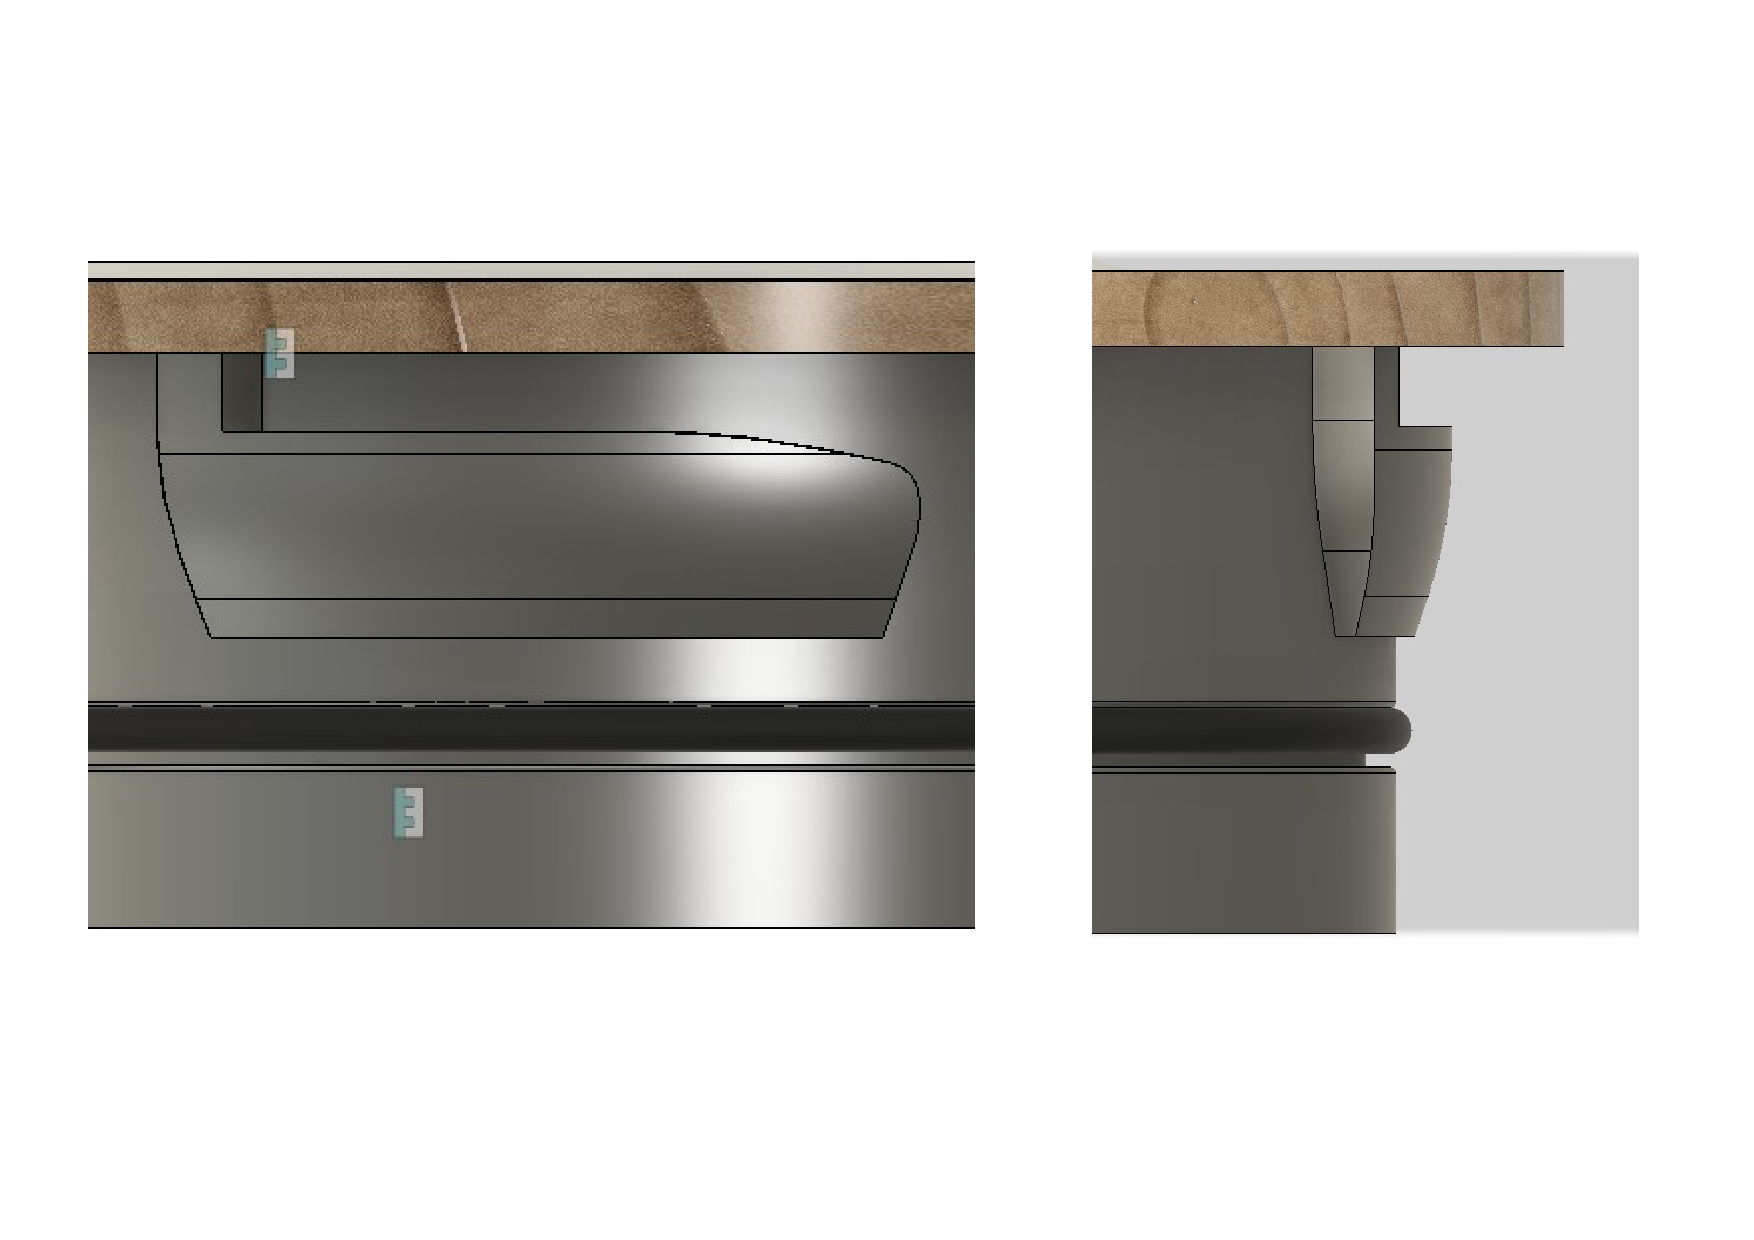
\includegraphics[width=400pt]{kapitoly/obrazky/E4/ukozy/ukladaci_ukosy.pdf}
    \caption{ukládací úkosy}
    \label{fig:E4-ukosy}
\end{figure}

\begin{figure}[htbp]
    \centering
    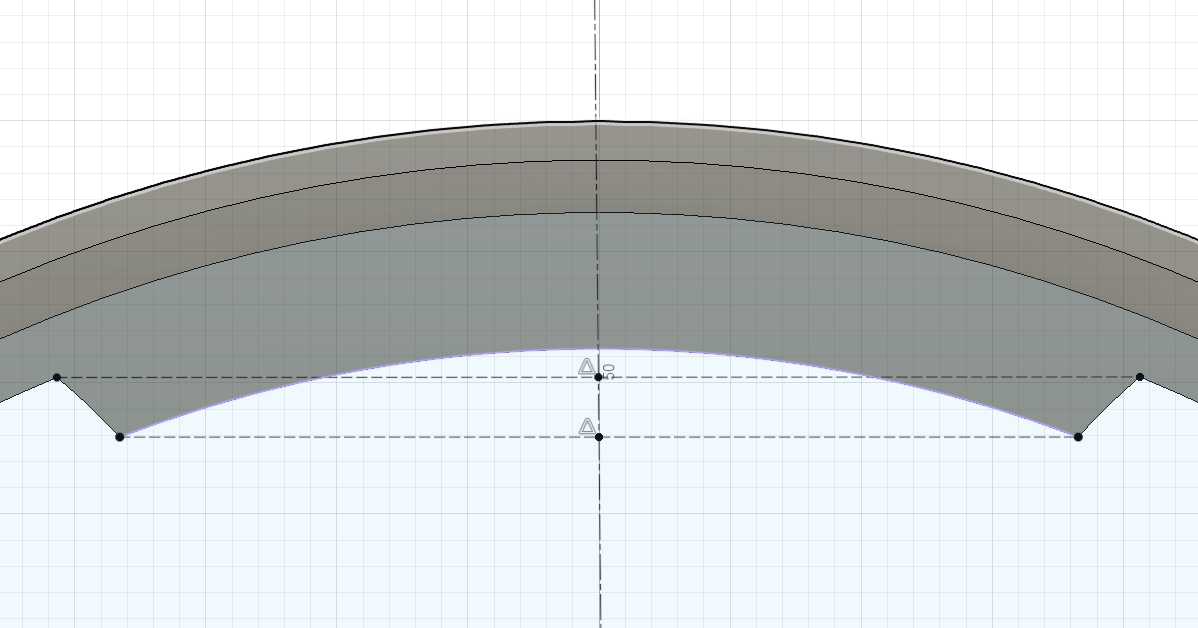
\includegraphics[width=400pt]{kapitoly/obrazky/E4/ukozy/simetrie_zarazek.png}
    \caption{Symetrie zarážky}
    \label{fig:E4-simetrie_zarazky}
\end{figure}
    Zarážky na obvodu otvoru mají obě kontaktní plochy stejné. Sice by mohlo být výhodné přizpůsobit tvar strany, kolem které se pohybuje západka, 
pohybu západky. Západka by tak mohla mít vedení v průběhu celého pohybu. Pro symetrii jsem se však rozhodl kvůli možnosti díl s otvorem otočit.
To je zvlášť výhodné při stavbě s dětmi, kvůli zmenšení počtu možných chyb, kterých se děti mohou při stavbě dopustit, a ztráta vedení není tak zásadní.


\clearpage
\newpage
\section{Elektronika tlakové desky}
\label{E4-tlakovka}
Tlaková plocha se díky pružné podložce a nažehlovací fólii může ve všech směrech naklánět, a díky tomu se při používání mění vzdálenost od čtyř snímacích
cívek. Tlaková plocha je primárně terčík, který slouží jako jádro cívky, která zvětšuje svou indukčnost, když se terčík přibližuje a naopak.

\begin{figure}[htbp]
    \centering
    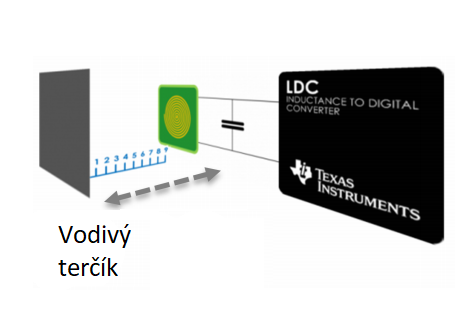
\includegraphics[width=200pt]{kapitoly/obrazky/E4/elektronika_tlakove_desky/civka_tercik_LDC.png}
    \caption{Schematické zobrazení cívky a terčíku \parencite{LDC-cd1}}
    \label{fig:E4-sch_civka_tercik}
\end{figure}

Pro snímání indukčnosti používám čip \href{https://www.ti.com/lit/ds/symlink/ldc1612.pdf?ts=1612018658531&ref_url=https%253A%252F%252Fwww.google.com%252F}{LDC1614} \parencite{LDC1614}
nebo \href{https://www.ti.com/lit/ds/symlink/ldc1312.pdf?ts=1612017390818&ref_url=https%253A%252F%252Fwww.google.com%252F}{LDC1314}, 
které se liší prakticky jen rozlišením. LDC1314 disponuje dvanáctibitovým AD převodníkem a LDC1614 dvacetiosmibitovým AD převodníkem 
a je tak schopen detekovat pohyb terčíku s rozlišením až na 10 nm.

\begin{figure}[htbp]
    \centering
    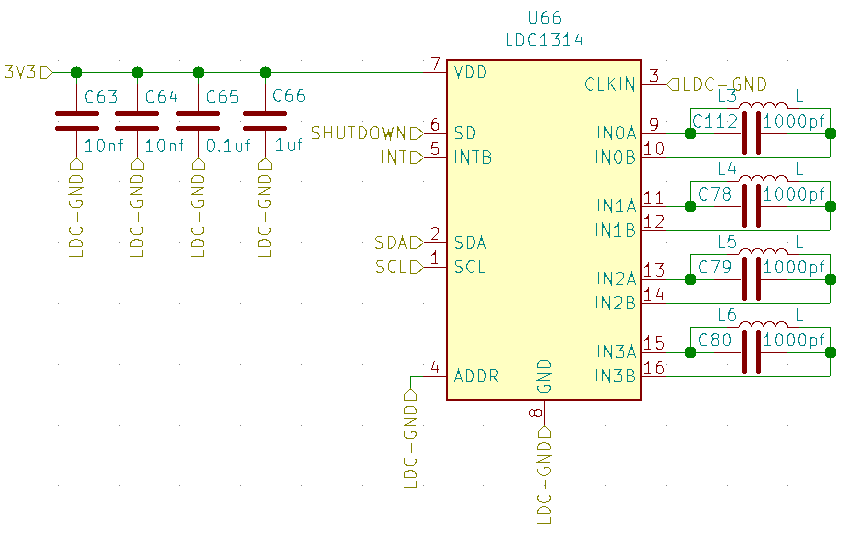
\includegraphics[width=\textwidth]{kapitoly/obrazky/E4/elektronika_tlakove_desky/moje_zapojeni.png}
    \caption{Zapojení čipu LDC1314 na desce trezoru}
    \label{fig:E4-LDC}
\end{figure}

Čip LDC komunikuje po sběrnici I2C, která umožňuje komunikaci jednoho mastera \footnote{čip, který řídí komunikaci} s až 128 slavy 
\footnote{čipy, které přijímají příkazy od mastra a pouze mu odpovídají}. LDC také umožňuje volbu ze dvou I2C adres, aby se dala adresa změnit v případná 
kolize s jiným čipem, který by měl stejnou adresu \footnote{např. aby se daly použít dva čipy LDC na jednom I2C}.

\newpage

Cívky použité na trezoru jsou vyrobeny jako reliéf ve vrstvě mědi přímo na DPS. Jejich vzhled jsem navrhoval v simulátoru od firmy Texas Instruments, 
vytvořeného konkrétně pro LDC čipy, a s pomocí popisů reálných aplikací \parencite{LDC-cd0} \parencite{LDC-cd1}, které firma Texas Instruments zveřejňuje.

% obrázek ze simulátoru

Výsledná cívka je vytvořena na dvouvrstvé desce a na každé vrstvě má patnáct závitů s drahou o síle 0,152~mm se stejně velkou mezerou, 
vzhled je vidět na obrázku \obr{fig:E4-relief_civka}.

Celý trezor obsahuje dvě samostatné elektronické desky, přičemž na jedné je osazen jen kruh z ledek WS2812 a snímání tlakové desky, které zabírá 
většinu této desky což je vidět na obrázku \obr{fig:E4-LedDeska}.

\newpage
\section{LED kruh}
\label{WS2812}

Trezoru vévodí světelný kruh. Slouží jako displej, na kterém trezor může zobrazovat vše, co potřebuje. Kruh obsahuje šedesát jednotlivých ledek 
\href{https://cdn-shop.adafruit.com/datasheets/WS2812B.pdf}{WS2812} \parencite{WS2812}, konkrétně variantu mini. Tuto variantu jsem zvolil, aby kruh mohl mít menší
průměr, který takto vychází na 80~mm. WS2812 mají totiž rozměr pouzdra 3,5x3,5~mm, zatím co ostatní varianty mají rozměry 5x5~mm \footnote{V průběhu vývoje se na trhu 
objevily i WS2812 v pouzdře 2020, které mají rozměru 2x2~mm ty však nebyly v nabídce JLCPCB a navíc byla deska již prakticky hotová.}, což by znamenalo průměr kruhu alespoň 120~mm.

WS2812 nejsou jen LED, ale májí v sobě logiku, díky které je možné jich řetězit velké množství za sebe. Díky tomu na řízení celého kruhu stačí jediný pin na ESP32.\newline
Ukázka PCB na obrázek \obr{fig:E4-LedDeska} a zapojení na \obr{fig:E4-sch_WS2812}.

Číslo šedesát jsem zvolil primárně kvůli zobrazování času, každá minuta v hodině nebo sekunda v minutě má tak svoji LED.
Zároveň toto číslo dobře navazuje i na zobrazování uhlů což koresponduje s magnetickým kompasem kterým BlackBox disponuje.

V momentální verzi softwaru se světelný kruh ovládá pomocí jedné z periferií ESP32, RMT a dá se používat ve dvou základních modech. 
V modu pro interakci s uživatelem označovaný jako DarkMode, který omezuje jas na 4\% \footnote{jas každého ze tří kanálů RGB 
se dá ovládat v rozmezí jednoho bajtu a v DarkMode je plný jas jen 10 místo 255} plného jasu, aby se na displej dalo koukat. 
Druhý mod je pak určen pro dálkovou signalizaci nebo pro prosté svícení a dokáže si říct až o 1.4 A.

\section{Napájení}
Jako napájení celého trezoru slouží dvě li-on baterie 18650. Napětí článků však nevyhovuje potřebám trezoru, a~tak je na trezoru lineární 
stabilizátor \href{https://datasheet.lcsc.com/szlcsc/1808280153_STMicroelectronics-LD39200PU33R_C222192.pdf}{NCP708} \parencite{LD39200}, 
který zajišťuje napětí 3,3~V pro většinu systému. Kromě LD39200 je zde také step-up \href{https://datasheet.lcsc.com/szlcsc/Feeling-Tech-FP6276AXR-G1_C83308.pdf}{FP6276} \parencite{fp6276}, 
který zajišťuje napájení 5~V sloužící primárně pro LED WS2812 a~v~druhá řadě napájí motor zámky,
jejich zapojení je přiloženo na obrázku \obr{fig:E4-sch_zdroj}.

\paragraph*{Zapínání}
\addcontentsline{toc}{paragraph}{Zapínání}
Aby se trezor mohl vypnout a~tak šetřit energii, je vybaven obvodem, který to umožňuje.

\footnote{vysvětlení funkce obvodu na obrázku \obr{fig:E4-zapinani}}Při připojení článků se napětí dostane nejprve na PTC \footnote{polymerová PTC, vratná pojistka } \parencite{polifuse},
které slouží jako ochrana proti nadproudu, například v případě, kdy uživatel připojí dva různě nabité články nebo jeden z~nich přepóluje.
Pokud se proud dostane skrz PTC, dostane se na tranzistor Q11 \parencite{power_MOSFET}, skrz který projde, jen pokud jsou články správně otočeny.
Když se napětí dostane přes ochranu proti přepólování, dostane se na S \footnote{SOURCE, vlastně EMITOR ale u unipolárního tranzistoru} 
tranzistoru Q5  \parencite{power_MOSFET}, skrz R6 na D \footnote{DRAIN, vlastně COLLECTOR ale u unipolárního tranzistoru} 
Q1 a~pak skrz R7 na obě strany C61.
Pokud v~takovéto situaci dojde ke~stisku SW3 , projde zem skrz C61 na G\footnote{GATE, vlastně BASE ale u unipolárního tranzistoru} Q5. 
V~tu~chvíli se Q5 otevře na dostatečně dlouhou dobu, 
aby naběhla třívoltová větev a~skrz pull-up \footnote{na obrázku je jen poznámka, reálná součástka je ve schematu společně s ESP32 na obrázku \obr{fig:E4-sch_ESP32}}
se zvedla napětí na G Q1 na téměř 3,3~V. Q1 se tak otevře a~už~trvale připojí GND na G Q5, trezor se tak zapnul. Pokud v takové chvíli procesor stáhne dráhu SHUTDOWN 3V3-5V 
na GND, nebo dojde ke stisku SW5, opět se uzavře Q1 a~skrz R6 projde na G Q5 napětí, které Q5 uzavře a~tak elektroniku opět vypne.

\begin{figure}[h]
    \centering
    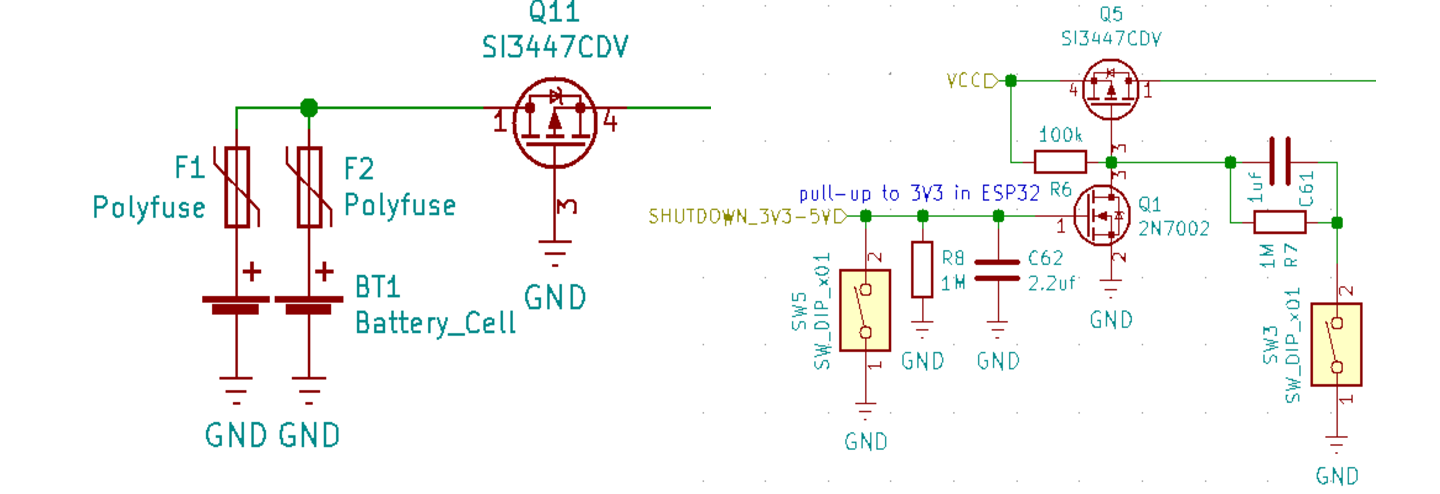
\includegraphics[width=\textwidth]{kapitoly/obrazky/E4/napajeni/ochrana_proti_prepolovani_a_zapinani.png}
    \caption{Ochrana proti přepólovaní a zapínání}
    \label{fig:E4-zapinani}
\end{figure}

\newpage

\paragraph*{Stabilizátor}
\addcontentsline{toc}{paragraph}{Stabilizátor}

Stabilizátor \href{https://datasheet.lcsc.com/szlcsc/1808280153_STMicroelectronics-LD39200PU33R_C222192.pdf}{LD39200} \parencite{ld39200} má pin EN, který slouží k~jeho vypínání. 
Pokud je na nem logická 0, je~stabilizátor vypnut a~pokud 1, je zapnut. Vzhledem k~tomu, že v~mém zapojení toto vypínaní nepotřebuji, je pin EN připojen 
přes R10 přímo na napájecí napětí, a~tak je stabilizátor trvale zapnut.
Konkrétně LD39200 jsem vybral kvůli malému pádu napětí, který vyžaduje pro svůj provoz, typicky 120~mV při proudu 1~A. Vzhledem k~tomu, že~na~vstupu 
mám maximálně 4,2~V, tak maximální napěťový pád, který mám k~dispozici je~0,9~V, protože na výstupu požaduji napětí 3,3~V. Navíc musím počítat 
i~s~vybitou baterií, u~které počítám s~napětím 3,5~V. %Rád bych počítal s~napětím ještě nižším, ale v~nabídce JLCPCB jsem nenašel stabilizátor s~nižším pádem napětí a~zároveň dostatečným proudem.

\begin{figure}[htbp]
    \centering
    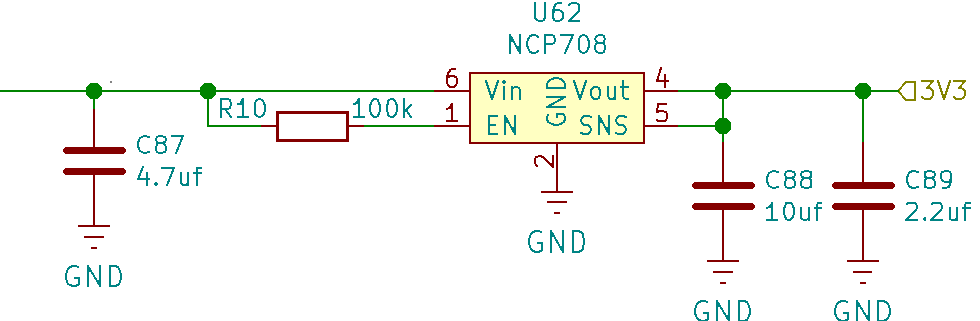
\includegraphics[width=400pt]{kapitoly/obrazky/E4/napajeni/stabilizator.png}
    \caption{Zapojení stabilizátoru}
    \label{fig:E4-stabilizator}
\end{figure}

\paragraph*{Step-up}
\addcontentsline{toc}{paragraph}{Step-up}

\subparagraph*{Step-up vysvětlení funkce}
Zapojení step-upu \footnote{spínaný zdroj který spíná vstupní napětí na napětí vyšší} je~o~něco složitější než stabilizátor, který stačí připojit a funguje. 
Spínané zdroje využívají ke své funkci cívku, na které vzniká změna napětí. Proud cívkou se nedá okamžitě zastavit a právě toho se využívá. 
Když se step-up spustí, připne výstup cívky k~zemi. Ve chvíli, kdy napětí klesně pod zadanou úroveň \footnote{předpokládá se že je v tu chvíli proud cívkou dostatečný}, 
přepne se výstup cívky na výstup step-upu.
Protože proud cívkou se nedá zastavit a~cívkou už proud teče, zvedne se napětí za cívkou, které začne plnit kondenzátor na výstupu.
Když napětí stoupne nad horní hranici požadovaného napětí, výstup cívky se opět přepne na zem. Ve chvíli, kdy napětí na kondenzátorech opět 
klesne, tím že dodává proud, připojí se cívka. Protože se~na~dobu pádu napětí na~výstupním kondenzátoru, připojila cívka na~zem, obnovil 
se~v~ní~proud a~cyklus se tak může opakovat.

\subparagraph*{Step-up zapojení na desce trezoru} 

\footnote{vysvětlení funkce obvodu na obrázku \obr{fig:E4-step-up}}Pro ovládání spínání step-upu jsem zvolil \href{https://datasheet.lcsc.com/szlcsc/Feeling-Tech-FP6276AXR-G1_C83308.pdf}{FP6276}.
Tento obvod jsem zvolil, protože mi vyhovoval jak po stránce napětí tak po~stránce efektivity a~ceny a~zároveň byl v~nabídce firmy JLCPCB
\footnote{firma u~které jsem desky vyráběl a~osazoval}.
Obvod jsem z~většiny zapojil dle doporučení výrobce, mojí prací bylo vlastně jen správně určit hodnoty 
jednotlivých součástek. Na ovládání pinu EN, který FP6276 vypíná, jsem připojil pull-up k napájení a~pro možnost step-up vypnout tranzistor Q2 \parencite{cj3134k}. 
Pokud tedy procesor stáhne dráhu SHUTDOWN 5V k zemi a~tak přivede na G\footnote{GATE, vlastně BASE ale u unipolárního tranzistoru} Q2 zem, 
Q2 se zavře a~tím se na pin EN přivede skrz R18 napájecí napětí, které step-up spustí. 
Pokud se na G Q2 přivede naopak logická jedna, Q2 se~otevře a~na~EN~se~dostane zem, která naopak provoz step-upu zastaví.

\begin{figure}[htbp]
    \centering
    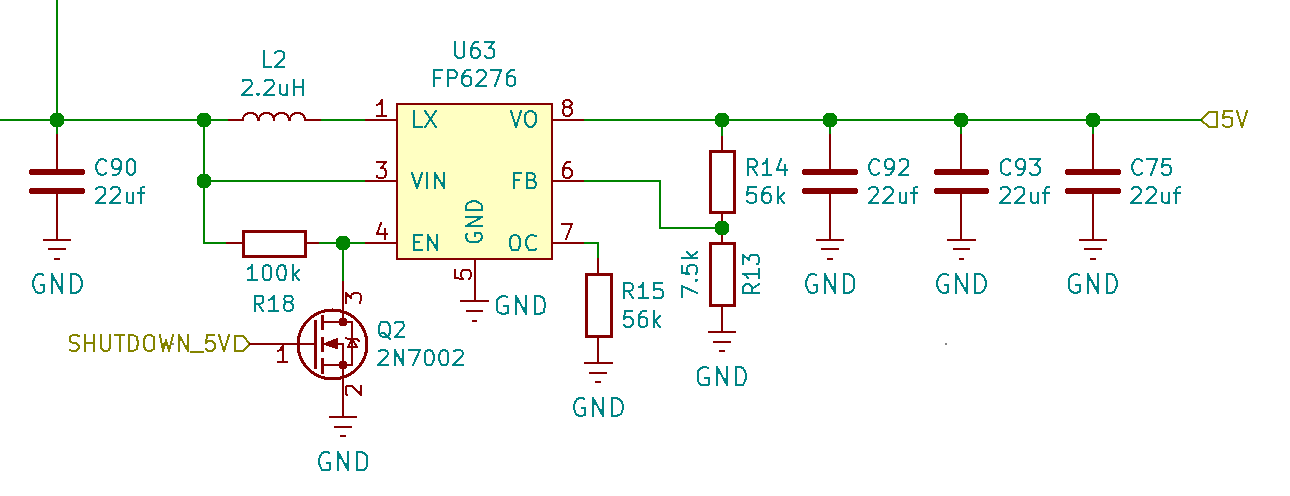
\includegraphics[width=400pt]{kapitoly/obrazky/E4/napajeni/step-up.png}
    \caption{Zapojení step-upu}
    \label{fig:E4-step-up}
\end{figure}

\newpage

\paragraph*{Měření napětí baterií}
\addcontentsline{toc}{paragraph}{měření napětí baterek}

\begin{wrapfigure}{R}{0.4\textwidth}
    \centering
    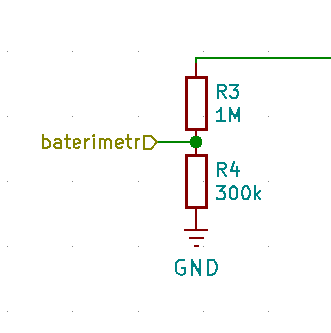
\includegraphics[width=0.4\textwidth]{kapitoly/obrazky/E4/napajeni/delic_baterimetru.png}
    \caption{Měření napětí baterií\label{fig:frog1}}
\end{wrapfigure}

Aby trezor mohl zjistit že má vybité baterie, musí mít možnost jim měřit napětí. ESP32 obsahuje AD převodník takže není problém měřit napětí baterie 
i poměrně přesně, kde však problem nastává, je maximální napětí, které je schopen měřit, a~to 1,1~V. ESP32 sice má možnost připojit k~AD převodníku dělič,
aby se~na~pin dalo přivést napětí až 3,3~V, ale to~pořád není dostatečné, a~také se~tím snižuje přesnost měření. Proto je na desce jednoduchý dělič napětí
složený ze~dvou odporů, jednoho s~hodnotou 1~M$\Omega$ a~druhého 300~k$\Omega$, takže při plně nabitých bateriích bude na výstupu děliče 0,97~V. %todo kolik je tam těch baterek. <- nevim jak to tam teď elegantně dopsat a ani bych to nepovažoval za nějak zvlášť podstatnou informaci v odstavci o měření napětí, je to hned v první větě pod nadpisem napájení

\newpage
\section*{Nabíjeni}
\addcontentsline{toc}{section}{Nabíjeni}

Aby se dveře trezoru nemuseli pokaždé rozebírat kvůli nabíjení, je deska vybavena lineární nabíječkou 
\href{https://datasheet.lcsc.com/szlcsc/Seaward-Elec-SE9017-HF_C115752.pdf}{SE9017}. 
Tuto nabíjecí obvod jsem zvolil z~nabídky JLCPCB kvůli volitelnému nabíjecímu proudu, který jsem pomocí R48 stanovil na 700 mA, a~také, kvůli malému 
pouzdru a~nízké ceně.
Pro signalizaci zda je~baterie dobita nebo zda se ještě dobijí jsou zde dvě LED~diodi LED4 a~LED5. Když se baterie dobíjí tak svítí LED4, která svítí 
červená, a~když je~baterie dobita svítí LED5, která svítí modře.

\begin{figure}[htbp]
    \centering
    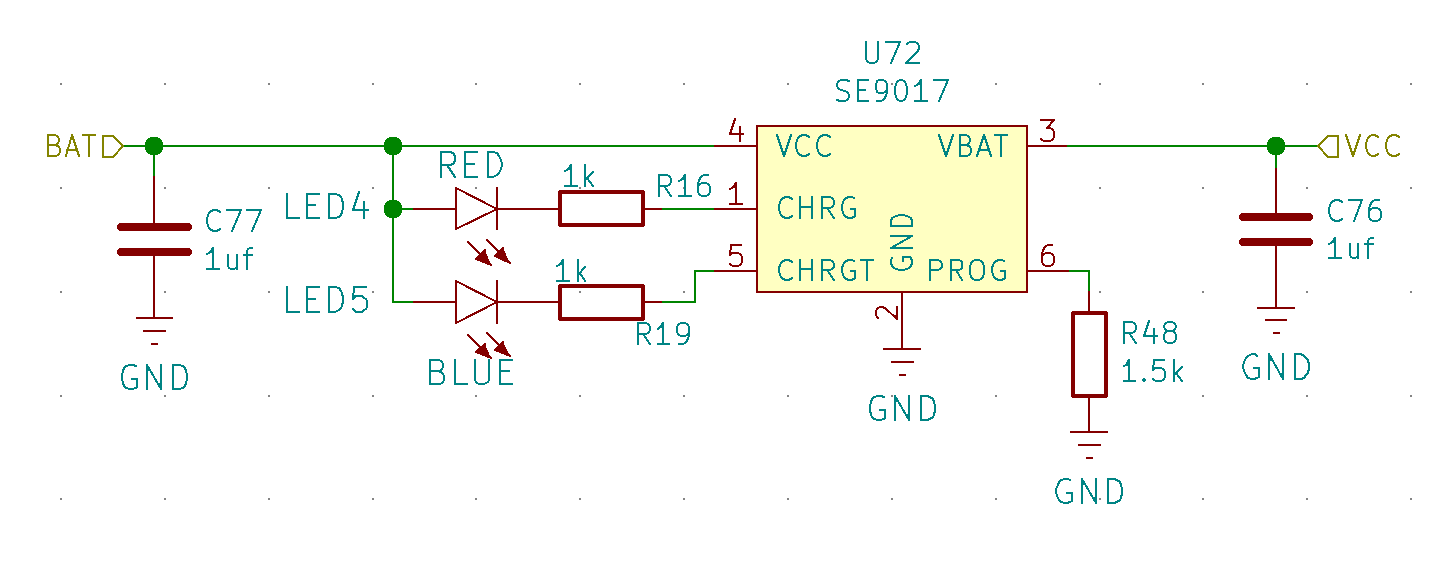
\includegraphics[width=\textwidth]{kapitoly/obrazky/E4/nabijeni/nabijecka.png}
    \caption{zapojeni nabíječky}
    \label{fig:E4-step-up}
\end{figure}

\newpage
% nenapadá mě co víc říct?
\section{ESP32 a jeho programátor}

\begin{wrapfigure}{L}[10mm]{0.4\textwidth}
    \centering
    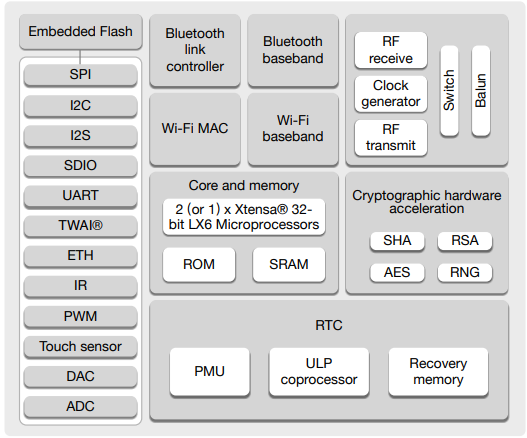
\includegraphics[width=0.4\textwidth]{kapitoly/obrazky/E4/ESP32/BlockDiagram.png}
    \caption{\label{fig:E4-ESP32-BlockDiagram}Zapínání a ochrana proti přepólovaní}
\end{wrapfigure}

Mozkem celého trezoru je~čip~\href{https://www.espressif.com/sites/default/files/documentation/esp32-wrover-b_datasheet_en.pdf}{ESP32-wrover} \parencite{ESP32-WROVER-B}. 
Obsahuje dva dva\-a\-tři\-ce\-ti\-bi\-to\-vé procesory Xtensa LX6 taktované až~na~240Mhz. ESP32 \parencite{ESP32} má také na modulu wrover k dispozici 520 KiB SRAM 
a~4,8 nebo 16~Mb flash paměti. ESP32 má také k~dispozici řadu periferií, z~nichž asi nejvýznamnější je WiFi a~Bluetooth. Právě integrace 
WiFi a~Bluetoothu je také jeden z~primárních důvodů volby tohoto čipu. Dalším podstatným důvodem volby čipu ESP32 je jeho vysoký výpočetní výkon, 
alespoň na poměry mikrokontrolérů a~v~neposlední řadě také fakt, že s~tímto čipem už nějakou dobu pracuji a~tak s ním již mám zkušenosti. 
Konkrétně wrover jsem pak zvolil kvůli dodatečné paměti PSRAM\footnote{Pseudo Static RAM} o velikosti 32 Mbit, 
\href{http://gamma.spb.ru/images/pdf/esp-psram32_datasheet_en.pdf}{ESP-PSRAM32} \parencite{ESP-PSRAM32}.

Kompletní zapojeni je na obrázku \obr{fig:E4-sch_ESP32}

ESP32 také vyžaduje mít při startu definované úrovně na některých pinech, proto jsou zde čtyři pull-upy\footnote{Rezistor je připojen mezi dráhu a napájení.} 
a dva pull-downy,\footnote{Rezistor je připojen mezi dráhu a zem.} které definují výchozí stav pinů IO0, IO2, IO5, IO12, IO15 a EN \parencite{ESP32}.
\begin{table}[h]
    \centering
    \resizebox{\textwidth}{!}{%
    \begin{tabular}{l|l|l}\midrule
    \textbf{IO0}    & ovládá boot procesoru             & LOW při resetu ESP vstupuje do bootloaderu    \\\midrule
    \textbf{IO2}    & potvrzení pro spuštění bootu      & LOW potvrzuje                                 \\\midrule
    \textbf{IO12}   & určuje napětí komunikace s flash  & LOW znamená napětí 3,3V a HIGH 1,8V           \\\midrule
    \textbf{IO15}   & ovládá zprávy bootloaderu do UART & LOW zprávy vypíná a HIGH zapíná               \\\midrule
    \textbf{EN}     & reset pin                         & LOW ESP je drženo v resetu                    \\\midrule
    \end{tabular}%
    }
    \caption{Popis funkce pinů}
    \label{tab:COMPARATION}
\end{table}

\subsection*{Programátor}
Aby mohl uživatel trezor jednoduše naprogramovat, je~na~desce převodník USB-UART, \href{https://www.silabs.com/documents/public/data-sheets/cp2102n-datasheet.pdf}{CP2102} \parencite{cp2102}.
Protože však CP2102 není potřeba celou dobu provozu a~protože trezor nemá k~dispozici neomezený zdroj elektřiny, je~převodník zapnut jen ve~chvíli, 
kdy je~připojeno USB-C , které slouží jak pro nabíjení, tak pro programování. Vypínání převodníku je zajištěno tranzistorem Q3, který je zároveň společně 
s~DIP~switchem SW4 využit pro možnost zákazu programování, viz obrázek \obr{fig:E4-sch_ESP32}.

\vspace{-3mm}
\section{Senzorika}
\vspace{-3mm}
Mezi podstatné funkce trezoru patří jeho vnímání veličin jako čas, jeho náklon nebo okolní tlak.
Deska proto obsahuje tři nebo čtyři čipy (v~závislosti na dostupnosti součástek), které trezoru poskytují gyroskop, akcelerometr, 
magnetický kompas,
barometr, RTC a~také konektor pro připojení modulu GPS a~GPRS. Díky těmto funkcím může trezor poskytnout možnost ovládání 
pomocí různých gest. 
Trezor třeba může sloužit, s~využitím magnetického kompasu a~LED kruhu, jako kompas, nebo se dá využít akcelerometr, 
aby se dal trezor odemknout jen v~konkrétním náklonu. 

Všechny čipy zobrazené na obrázku \obr{fig:E4-sch_senzorika} komunikují s~ESP32 hlavně pomocí 
sběrnice I2C. Pro možnost zrychlení reakcí má však každý z~čipů také pin určený pro spuštění přerušení na procesoru, zapojení najdete na obrázku \obr{fig:E4-sch_senzorika}. 
To je užitečné, protože komunikaci na I2C řídí ESP32. Pokud se tedy ESP32 nerozhodne zeptat se jiného čipu 
na jím naměřená data, čip mu to po I2C nemá 
jak sdělit. Zároveň se však procesor nemůže bez ustání ptát na měření ostatních čipů, protože by pak nestíhal dělat nic jiného. Proto jsou čipy vybaveny 
pinem, který změní svou logickou hodnotu ve chvíli, kdy naměřené hodnoty splní nějaké podmínky. 
Například může být trezor naprogramován, aby se otevřel 
v~konkrétní čas. Tento čas se potom dá nastavit v~RTC jako hodnota, při jejímž dosažení RTC přepne pin přerušení. ESP32 pak jen přečte logickou hodnotu 
pinu a~vlastně ani nemusí komunikovat po I2C.

\paragraph{Akcelerometr, gyroskop a~magnetický kompas}
\addcontentsline{toc}{paragraph}{Akcelerometr gyroskom a~magnetický kompas}
Tyto funkce trezor má pro možnost sledování své pozice v~prostoru. 
Díky akcelerometru má trezor k~dispozici informaci o~směru a~velikosti svého zrychlení v~prostoru.
Gyroskop poskytuje informaci o~relativním natočení trezoru, což se může využít jako další podmínka pro otevření trezoru nebo pro různá ovládací gesta.
Magnetický kompas pak pochopitelně dodává informaci o~natočení vůči zemskému magnetickému poli.

Na prvním prototypu verze E4 poskytoval akcelerometr, gyroskop i~magnetický kompas čip \href{https://datasheet.lcsc.com/szlcsc/Bosch-Sensortec-BMX055_C94022.pdf}{BMX055} \parencite{bmx055},
protože však tento čip nebyl jednoduše dostupný, přidal jsem na další verzi i~čip \href{https://datasheet.lcsc.com/szlcsc/TDK-InvenSense-MPU-6050_C24112.pdf}{MPU6050} \parencite{mpu6050},
který obsahuje akcelerometr a~gyroskop a~čip \href{https://datasheet.lcsc.com/szlcsc/QST-QMC5883L-TR_C192585.pdf}{QMC5883} \parencite{qmc5883}, který dodává magnetický kompas.
Na desce je tak místo pro všechny tři čipy, a~pokud není k~dispozici BMX055, jednoduše se osadí MPU6050 a~QMC5883. 

\begin{figure}[h]
    \centering
    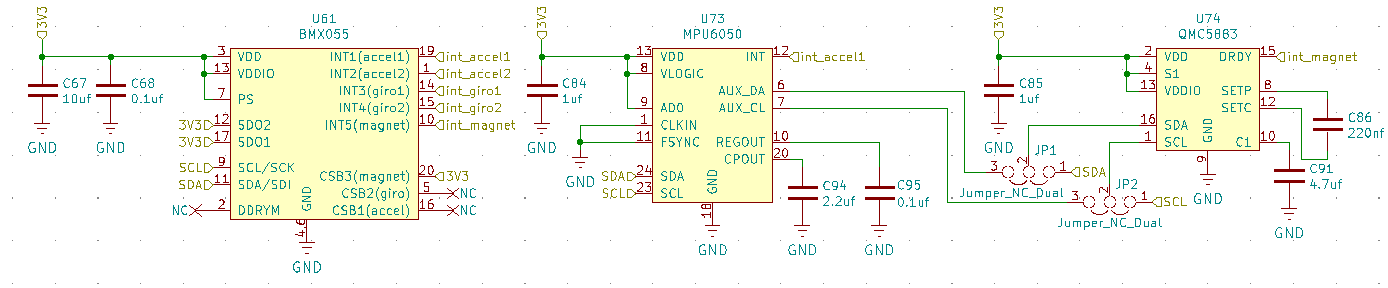
\includegraphics[width=\textwidth]{kapitoly/obrazky/E4/vnimani/BMX-MPU-QMC.png}
    \caption{Zapojení čipů BMX055, MPU6050 a~QMC5883}
    \label{fig:E4-9axis}
\end{figure}

\vspace{-5mm}

\subparagraph*{Akcelerometr}
\label{akcelerometr}
U~\ čipu \ BMX055 \ akcelerometr \ disponuje \ rozlišením \\ 1~mm$\cdot$s$^{-2}$ neboli 0,097m$g$ při rozsahu měření $\pm2g$. 
Jeho rozsah se ale dá nastavit, a~to na $\pm2g$, $\pm4g$, $\pm8g$, $\pm16g$, 
podle rozsahu se také mění přesnost měření. Přesnost je totiž omezena velikostí dvanáctibitového registru, do 
kterého se ukládají informace, a~při využívání většího 
rozsahu měření už tento registr není dostatečně velký, aby uchovával stejnou přesnost.

MPU6050 má vedle BMX u~akcelerometru stejné rozsahy měření, disponuje však šestnáctibitovými registry, a~tak je 
sto dosáhnout i~vetší přesnosti. Jeho maximální rozlišení je 
tak 60$\mu g$. Výměnou čipu BMX055 za čip MPU6050 jsem si tak polepšil i~po straně přesnosti, přesto, že tuto přesnost 
pravděpo\-dob\-ně nikdy BlackBox nevyužije. %todo jakože určitě ne ale přijde mi to divný zmiňovat i takhle mi to přijde jakési nekulantní ale možná je to zlozvyk z prezentace

\subparagraph*{Gyroskop}
\label{gyroskop}
U~čipu BMX055 je gyroskop sto poskytovat informaci o~úhlo\-vé rychlosti s~rozlišením na 0,004°\!/s,
 opět ale záleží na rozsahu měření kvůli stále stejné velikosti 
dvanáctibitového registru. 
Můžete si u~něj vybrat z~rozsahu $\pm125$°\!/s, $\pm250$°\!/s, $\pm500$°\!/s, $\pm1 000$°\!/s, $\pm2 000$°\!/s.

Po přechodu na čip MPU6050 jsem si opět po polepšil po straně přesnosti, i~u~gyroskopu totiž disponuje 
šestnáctibitovými registry a~rozsahy měření jsou opět stejné jako u~BMX055.

\subparagraph*{Magnetický kompas}
\label{magnetometr}
Čip BMX055 je sto měřit sílu magnetického pole s~přesností až na  0,3~$\mu$T 
v~rozsahu $\pm$1200~$\mu$T u~os $x$ a~$y$, u~osy $z$~pak v~rozsahu $\pm$2500~$\mu$T.

Magnetometr, který poskytuje čip QMC5883, pak měří v~rozsahu $\pm8$~Gs, což pro srovnání 
odpovídá $\pm$800~$\mu$T a~s~přesností až $2$~mGs opět pro srovnání to odpovídá $\pm$0,2~$\mu$T.
Na rozdíl od BMX055 se u~QMC5883 dá volit rozsah měření, a~tak si můžete vybrat z~$\pm2$~Gs 
a~nebo ze zmíněních $\pm8$~Gs.

%\newpage

\paragraph{Barometr, teploměr}
\addcontentsline{toc}{paragraph}{Barometr}
\label{barometr}
Barometr poskytuje informaci o~okolním atmosferickém tlaku. 
Tato informace může sloužit pro rozeznávání nadmořské výšky. 
BlackBox tak může sloužit i~jako jednoduchá meteorologická stanice, s~možností měření tlaku i~teploty (viz dále).

Od doby, kdy jsem z~nabídky JLCPCB vybíral čip 
\href{https://datasheet.lcsc.com/szlcsc/1907081118_Goertek-SPL06-007_C233787.pdf}{SPL06}, 
JLCPCB doplnilo do své nabídky několik dalších barometrů a~dneska bych tedy dost možná zvolil jiný. 
Každopádně tehdy jsem volil 
mezi dvěma čipy, které byly v~nabídce JLCPCB dostupné a~SPL06 měl vyšší rozlišení a~byl za téměř stejnou cenu.

SPL06 je sto měřit tlak v~rozsahu 950 až 1050~hPa s~přesností na 0,06~hPa 
a~je tak sto poznat změnu nadmořské výšky o~0,5~m.

SPL06 má také vedle barometru i~teploměr, který je sto měřit teplotu od -40°C do 85°C s~rozlišením na 0,01°C.

\begin{figure}[h]
    \centering
    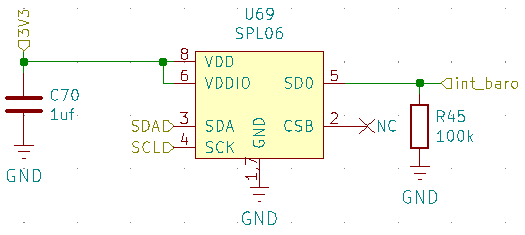
\includegraphics[width=\textwidth]{kapitoly/obrazky/E4/vnimani/SPL06.png}
    \caption{Zapojení čipu SPL06}
    \label{fig:E4-SPL06}
\end{figure}

\newpage

\paragraph{RTC}
\addcontentsline{toc}{paragraph}{RTC}
\label{RTC}
Aby si trezor mohl zachovávat povědomí o~aktuálním čase i~ve chvíli, kdy je vypnut, má k~dispozici čip 
\href{https://datasheet.lcsc.com/szlcsc/STMicroelectronics-M41T62Q6F_C113207.pdf}{M41T62} \parencite{m41t62}.

RTC je napájeno přímo z~baterie, hned za ochranou proti přepólování, aby bylo sto uchovávat čas i~ve vypnutém stavu.
Z~toho důvodu jistě potěší nízká spotřeba 350 nA ve chvíli, kdy jen uchovává čas a~35 µA ve chvíli, kdy je aktivní I2C.
Maximální odchylka od skutečného času může být 5~s~za měsíc provozu.

\begin{figure}[h]
    \centering
    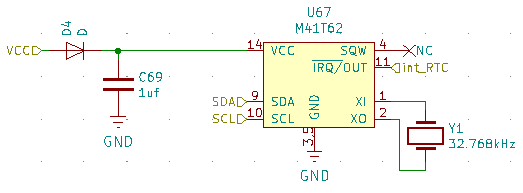
\includegraphics[width=\textwidth]{kapitoly/obrazky/E4/vnimani/RTC.png}
    \caption{Zapojení čipu M41T62}
    \label{fig:E4-M41T62}
\end{figure}

\newpage

\paragraph{Konektor pro GPS/GPRS modul}
\label{A9}
Ve chvíli, kdy jsem na trezor do\-pl\-ňo\-val čipy MPU6050 a~QMC5883, jsem zároveň doplnil i~tento konektor. 
Ve verzi, která je osazena MPU6050 a~QMC5883, a~nemá tedy osazen čip BMX055, 
je totiž více volných pinů. BMX055 totiž využívá pět pinů přerušení, zatím co MPU6050 a~QMC5883 mají každý po jednom. 
Proto při nevyužití BMX055 zbudou tři volné piny.
Protože čip A9G\footnote{Čip využívám jako GPS a~GPRS modul.} komunikuje po sběrnici UART, na rozdíl od ostatních čipu na desce. 
Pro UART však potřebuji
dva piny a~ty kolidují s~piny přerušení čipu BMX055. Proto se konektor dá použít, jen pokud není osazen BMX055.

\begin{figure}[h]
    \centering
    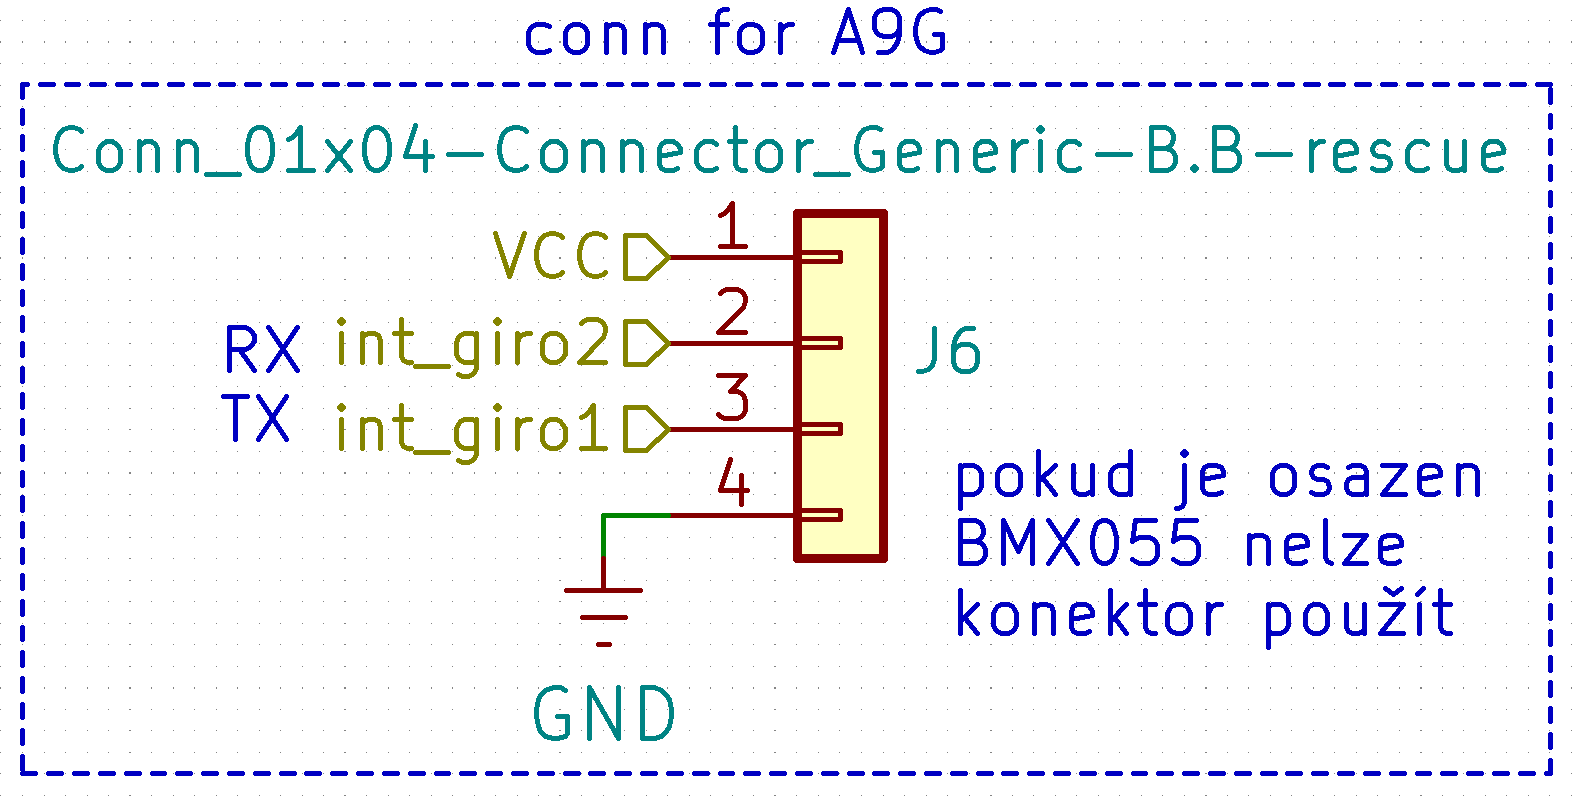
\includegraphics[width=\textwidth]{kapitoly/obrazky/E4/vnimani/conn-A9G.png}
    \caption{Zapojení konektoru pro A9G}
    \label{fig:E4-A9G}
\end{figure}


\section{Ovládání západky a IR komunikace}

Zapojení je dostupné na obrázku \obr{fig:E4-sch_IR-Motor-enkoder}.

\paragraph{IR komunikace}
\addcontentsline{toc}{paragraph}{IR komunikace}
IR slouží primárně pro identifikaci dveří, při vkládání většího množství dveří do stejného trezoru.
Trezor totiž počítá s možností vkládání více dveří do jednoho trezoru, což je jedna ze schopností, kterou více použije trezor jako hračka, než trezor jako bezpečnostní schránka.
Tento trezor s více dveřmi by zároveň mohl sloužit jako jakýsi displej a na to potřebuje vědět, které dveře jsou kde, na což slouží právě IR komunikace. %todo ???? <- ???

Jako IR přijímač jsem z nabídky JLCPCB \parencite{JLCPCB} zvolil \href{https://datasheet.lcsc.com/szlcsc/1912111437_Everlight-Elec-IRM-H936-TR2_C264266.pdf}{IRM-H936} \parencite{irm-h936}. 
V nabídce JLCPCB byly v době nárhu desky jen dva IR při\-jí\-ma\-če, právě IRM-H936 a \href{https://datasheet.lcsc.com/szlcsc/2010221806_Everlight-Elec-IRM-H638T-TR2-DX_C390031.pdf}{IRM-H638},
z nichž IRM-H936 má skoro poloviční výšku a širší úhel záběru, a to byl důvod jeho volby.

Druhou částí IR komunikace je vysílač, který je zajištěn jednoduše IR LED \parencite{ir19-21c/tr8}.

\begin{figure}[htbp]
    \centering
    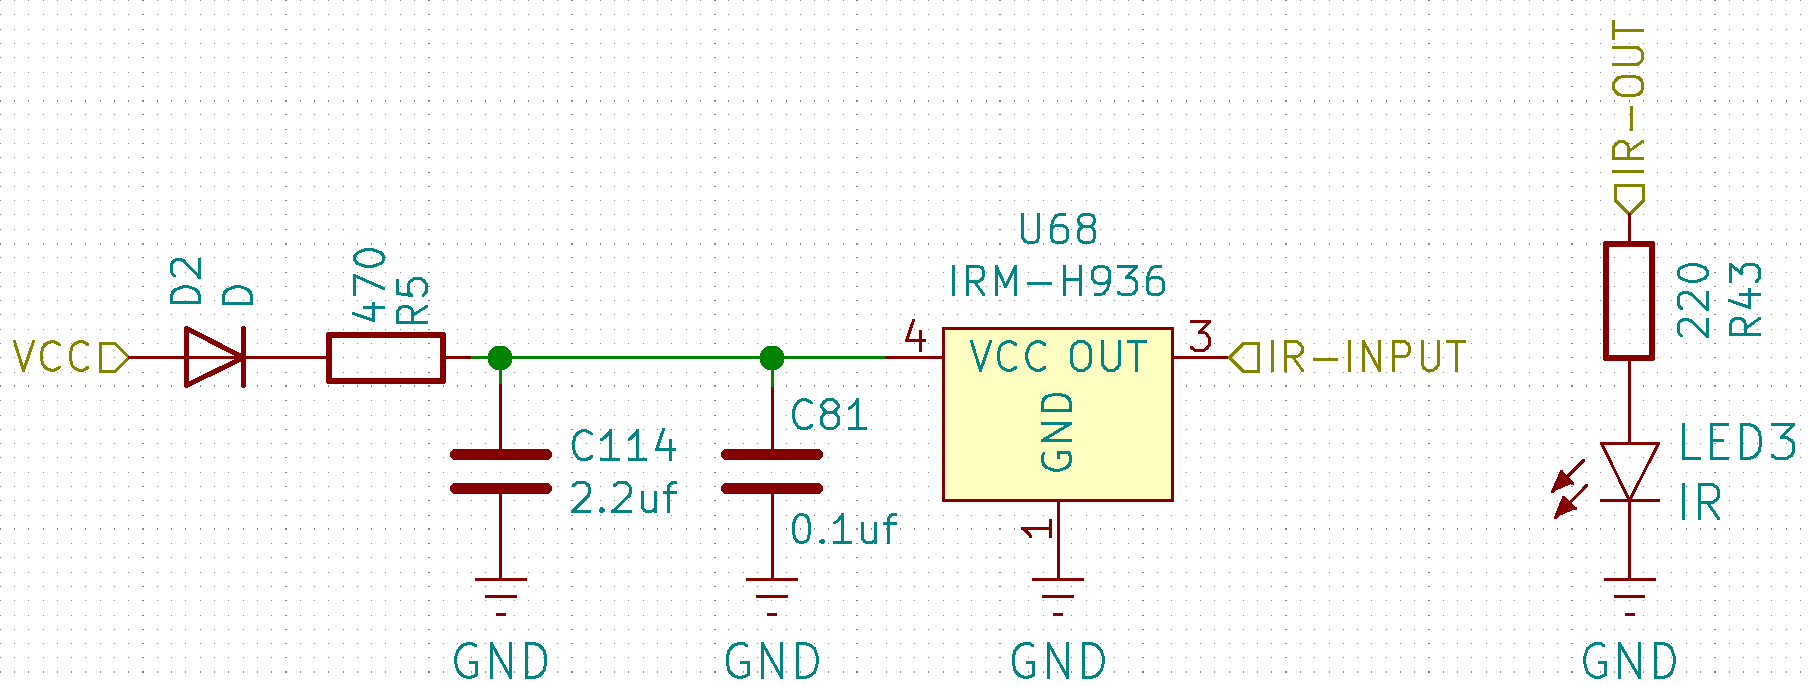
\includegraphics[width=\textwidth]{kapitoly/obrazky/E4/ir_motor_enkoder/IR.png}
    \caption{Zapojení IR vysílače a přijímače}
    \label{fig:E4-ir}
\end{figure}

\newpage

\paragraph{Ovládání motoru}
\addcontentsline{toc}{paragraph}{Ovládání motoru}
Protože motor je napájen z 5~V větve a protože ho připínám k napájení a ne k zemi, nemůžu ho ovládat přímo z procesoru. Proto je Q7 napojen na Q10, který je teprve řízen z~ESP. 
Kvůli napěťovým špičkám, které při běhu vznikají na komutátoru motoru, je zde i zpětná Schottkyho dioda, D3.

Motor bych sice mohl napájet z napětí 3,3~V a nemusel bych tím pádem přidávat tranzistor navíc, ale zároveň bych tím zpomalil rychlost motoru.\footnote{otáčky motoru ale přes to mohu snížit dle potřeby}
Další možností by bylo napájet motor přímo z napětí na bateriích a mohl bych tak motor spustit i bez zapnutí 5~V zdroje. To by však znamenalo nutnost 
sofistikovanějšího řízení motoru, protože by se motor točil různou rychlostí v~závislosti na nabití baterií.

\begin{figure}[htbp]
    \centering
    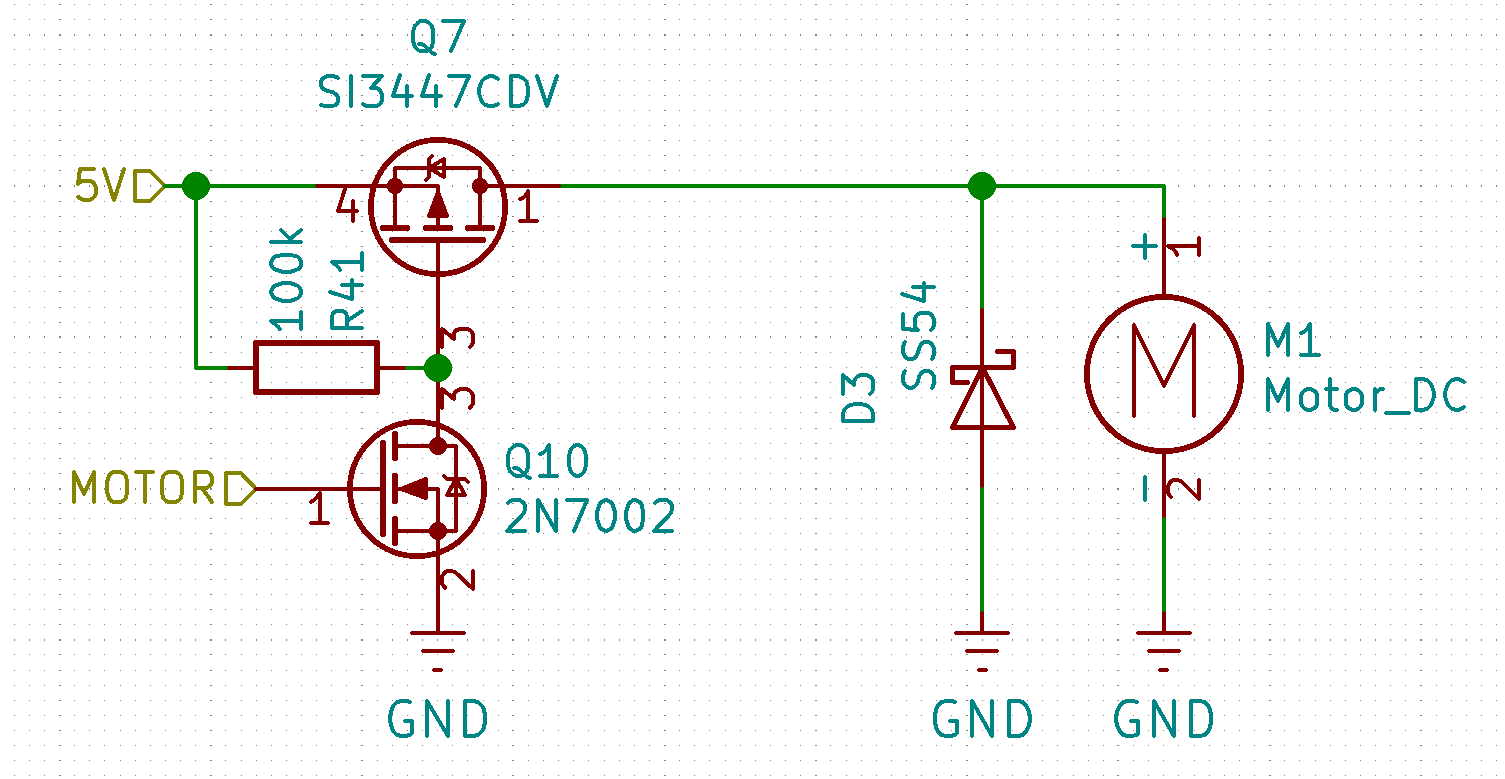
\includegraphics[width=\textwidth]{kapitoly/obrazky/E4/ir_motor_enkoder/ovladani_motoru.png}
    \caption{Zapojení řízení motoru}
    \label{fig:E4-motor}
\end{figure}



\paragraph{Enkodér}
\addcontentsline{toc}{paragraph}{Enkoder}

\begin{wrapfigure}[13]{R}{0.65\textwidth}
    \centering
    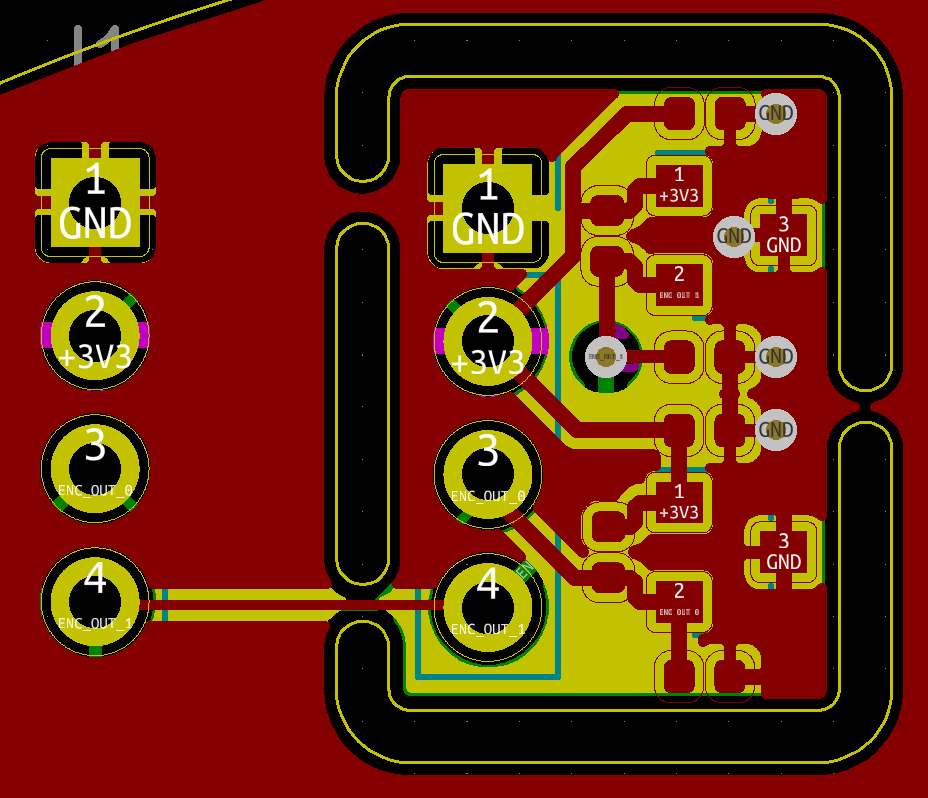
\includegraphics[width= 0.6\textwidth]{kapitoly/obrazky/E4/ir_motor_enkoder/pcb-enc.png}
    \caption{\label{fig:E4-enkoder_pcb}Vzhled enkorédu na desce}
\end{wrapfigure}
Aby bylo možno motor polohovat do správné polohy, je nutné mít zpětnou vazbu o~jeho poloze. Vzhledem k~tomu, že motor otáčí magnetem, samo se nabízí využít magnetický enkodér. 
Proto jsou na desce dvě digitální Hallovy sondy \href{https://datasheet.lcsc.com/szlcsc/Honeywell-SS360ST_C111924.pdf}{SS360NT} \parencite{ss360nt}, které se překlopí podle toho, 
u jakého magentického pólu se nachází. 

Na desce s~LED kruhem by sondy musely být na opačné straně než LED, takže by se musely pájet ručně, protože JLCPCB osazuje jen z~je\-dné strany. Hlavní deska je ale zase, 
kvůli velikosti baterií, moc daleko od magnetu. 

Abych tedy nemusel dělat třetí desku jen kvůli enkodéru, zvolil jsem možnost vylomitelného enkodéru. Na hlavní desce jsem tedy nakreslil 
enkodér s konektorem a objel jsem ho frézou, aby se dal při montáži trezoru z desky vylomit a posunout do ideální polohy.
Vzhled enkodéru je vidět v~horní části obrázku \obr{fig:E4-MainBoard}

\begin{figure}[htbp]
    \centering
    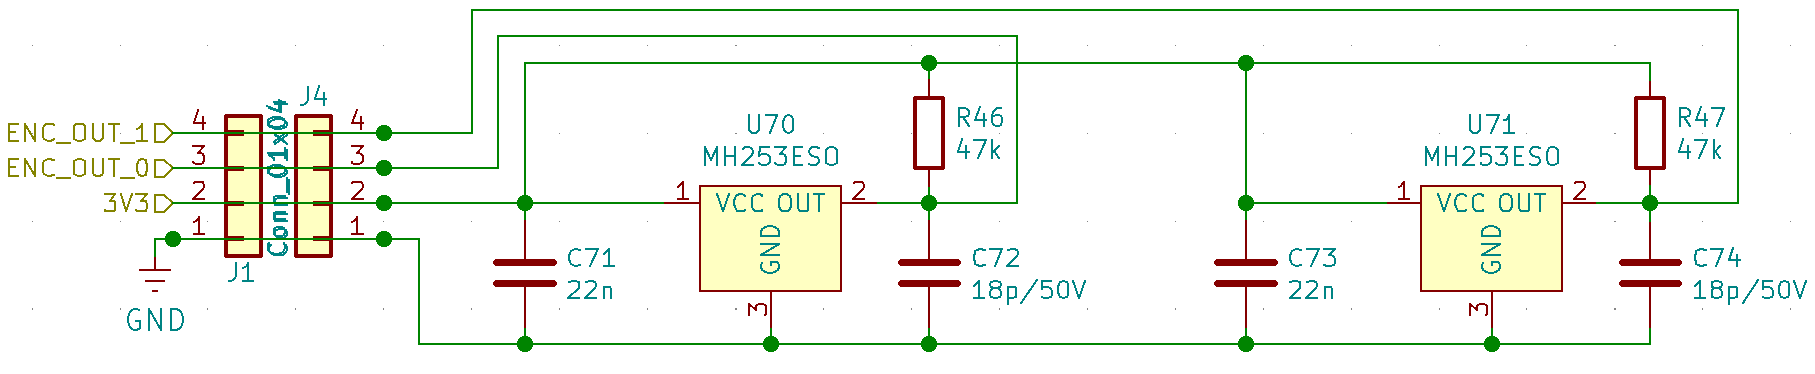
\includegraphics[width=\textwidth]{kapitoly/obrazky/E4/ir_motor_enkoder/enc.png}
    \caption{Zapojení enkodéru}
    \label{fig:E4-enkoder}
\end{figure}

\newpage
\section{Výroba mechanických dílů}
Prototypové verze trezoru jsem vyráběl pomocí laserové řezačky a~3D~tisku, a~to technologiemi \href{https://www.3dhubs.com/guides/3d-printing/#fdm}{FDM} 
a~\href{https://www.3dhubs.com/guides/3d-printing/#sla-dlp}{SLA}. 
Po odzkoušení prototypů jsem však u 3D tisknutých dílů přešel na odlévání polyuretanu do silikonové formy. 

\paragraph*{Výroba silikonové formy}
Před tím, než se dá začít odlévat hotový díl, musí se pochopitelně udělat forma. 
Jako materiál formy jsem zvolil silikon pro jeho pružnost. 
Ta mi umožňuje odlévat i záporné převisy, u kterých bych musel běžnou formu rozdělit na velké množství dílů.
Konkrétně jsem zvolil dva lukoprény \href{https://www.lucebni.cz/cs/lukopren-n/49-silikonovy-kaucuk-lukopren-n-8200.html}{N8200} 
a \href{https://www.lucebni.cz/cs/lukopren-n/43-silikonovy-kaucuk-lukopren-n-5221.html}{N5221}, který používám na formy různých dílů.
N8200 je totiž ve srovnání s N5221 odolnější ale má vyšší viskozitu a tak nezateče do úzkých skulin.
Proto na některé formy používám N8200 a na jiné N5221, abych formu byl vůbec sto vyrobit. 
Forma na odlévání těla dveří dokonce kombinuje oba dva, jelikož je dvoudílná a jeden z dílů je tvarově náročný.

Abych ale mohl formu vyrobit, potřebuji mít vyrobené 
kopyto\footnote{Forma určená pro výrobu další formy.}. Abych jej získal, využil jsem znovu 3D tisku.
Tentokráte 3D tisk SLA, který umožňuje dosažení daleko vyšší přesnosti než technologie FDM. %todo mám popisovat i specifické technologické úpravy pro SLA?
Do vyrobeného kopyta se naleje dobře promíchaná a vyvakuovaná směs kaučukové pasty a katalyzátoru.
Ta se následně nechá zvulkanizovat a vyjme se z kopyta.

Při odlévání vícedílné formy, ve chvíli, kdy se jeden díl odlévá podle již hotového dílu, je třeba natřít kontaktní plochy na hotovém díle separátorem, aby se výsledek neslepil.
Pro tento účel jsem používal \href{https://www.lucebni.cz/cs/pomocne-pripravky/54-lukopren-parafinovy-separator.html}{parafínový separátor}.

\paragraph*{Odlévání polyuretanu}
Konkrétně jsem zvolil polyuretan \href{https://www.smooth-on.com/tb/files/TASK_4_TB.pdf}{TASK 4} s vyvá\-že\-ný\-mi mechanickými i technologickými vlastnostmi.
Složky polyuretanu se smísí a ve vakuové komoře řádně promíchají. Následně se polyuretan nalije do formy a vloží do přetlakové komory,
protože polyuretany jsou sto, za zvýšeného tlaku, pohltit nějaké množství vzduchu.
Zbylé vzduchové bublinky, které se do polyuretanu dostaly, se tak v polyuretanu rozpustí.

\newpage
\chapter{Využití}
\section{Použití trezoru}
První nasazení trezoru na akci pořádané Robotárnou \parencite{robotarna} proběhla na příměstském robotickém táboře v srpnu roku 2019.
Jednalo se o první variantu trezoru která kdy spatřila světlo světa \ref{E1-vyvoj}. Tábor trval pět dní a děti dostali první tři dny na stavbu mechaniky a poslední dva dny 
se~programovalo. 

Trezor tehdy sklidil úspěch a tak započal vývoj dalších verzí které už byli specializovanější \ref{E2-vyvoj} \ref{E3-vyvoj} a přidali se i mechanické
varianty \ref{M1-vyvoj} \ref{M2-vyvoj} \ref{M3-vyvoj}.

\paragraph{Trezor ve volnočasových kurzek robotiky}
Další používání trezoru probíhalo v jednom volnočasovém kurzu robotiky který jsem spoluvedl a účastníci v něm stavěli nejprve tehdy aktuální mechanickou variantu, verzi M2 \ref{M2-vyvoj}.
Protože účastníci kurzu byli vetšinou již docela zkušení, jednalo se u nimi téměř jen o \uv{rozcvičku} kterou měli za několik kroužků hotovou a následovala stavba trezoru E3. 

Bohužel kvůli pandemickým opatřením si ne všichni účastníci stihli trezor postavit a vůbec jsme se nedostali k programování, natož aby jsme si s trezorem zorganizovali nějakou herní akci, 
jak bylo dříve v plánu.

\paragraph{Trpasličí trezor}
Chvíli po té co vznikl trezor M3 \ref{M3-vyvoj} \ref{M3-popis} proběhla první akce s trezorem které nebyla pod taktovkou Robotárny \parencite{robotarna}. Zároveň to byla také 
první akce na které se trezor nestavěl a jen se využíval.

Protože na akci byly menší děti, byl trezor místo klasické číselné stupnice  vybaven obrázkovým kódem, jak je vidět na obrázku \obr{fig:M3-trpaslici}.

Toto však byla poslední akce která se stihla uskutečnit před započetím pandemických opatření.

\begin{figure}[htbp]
    \centering
    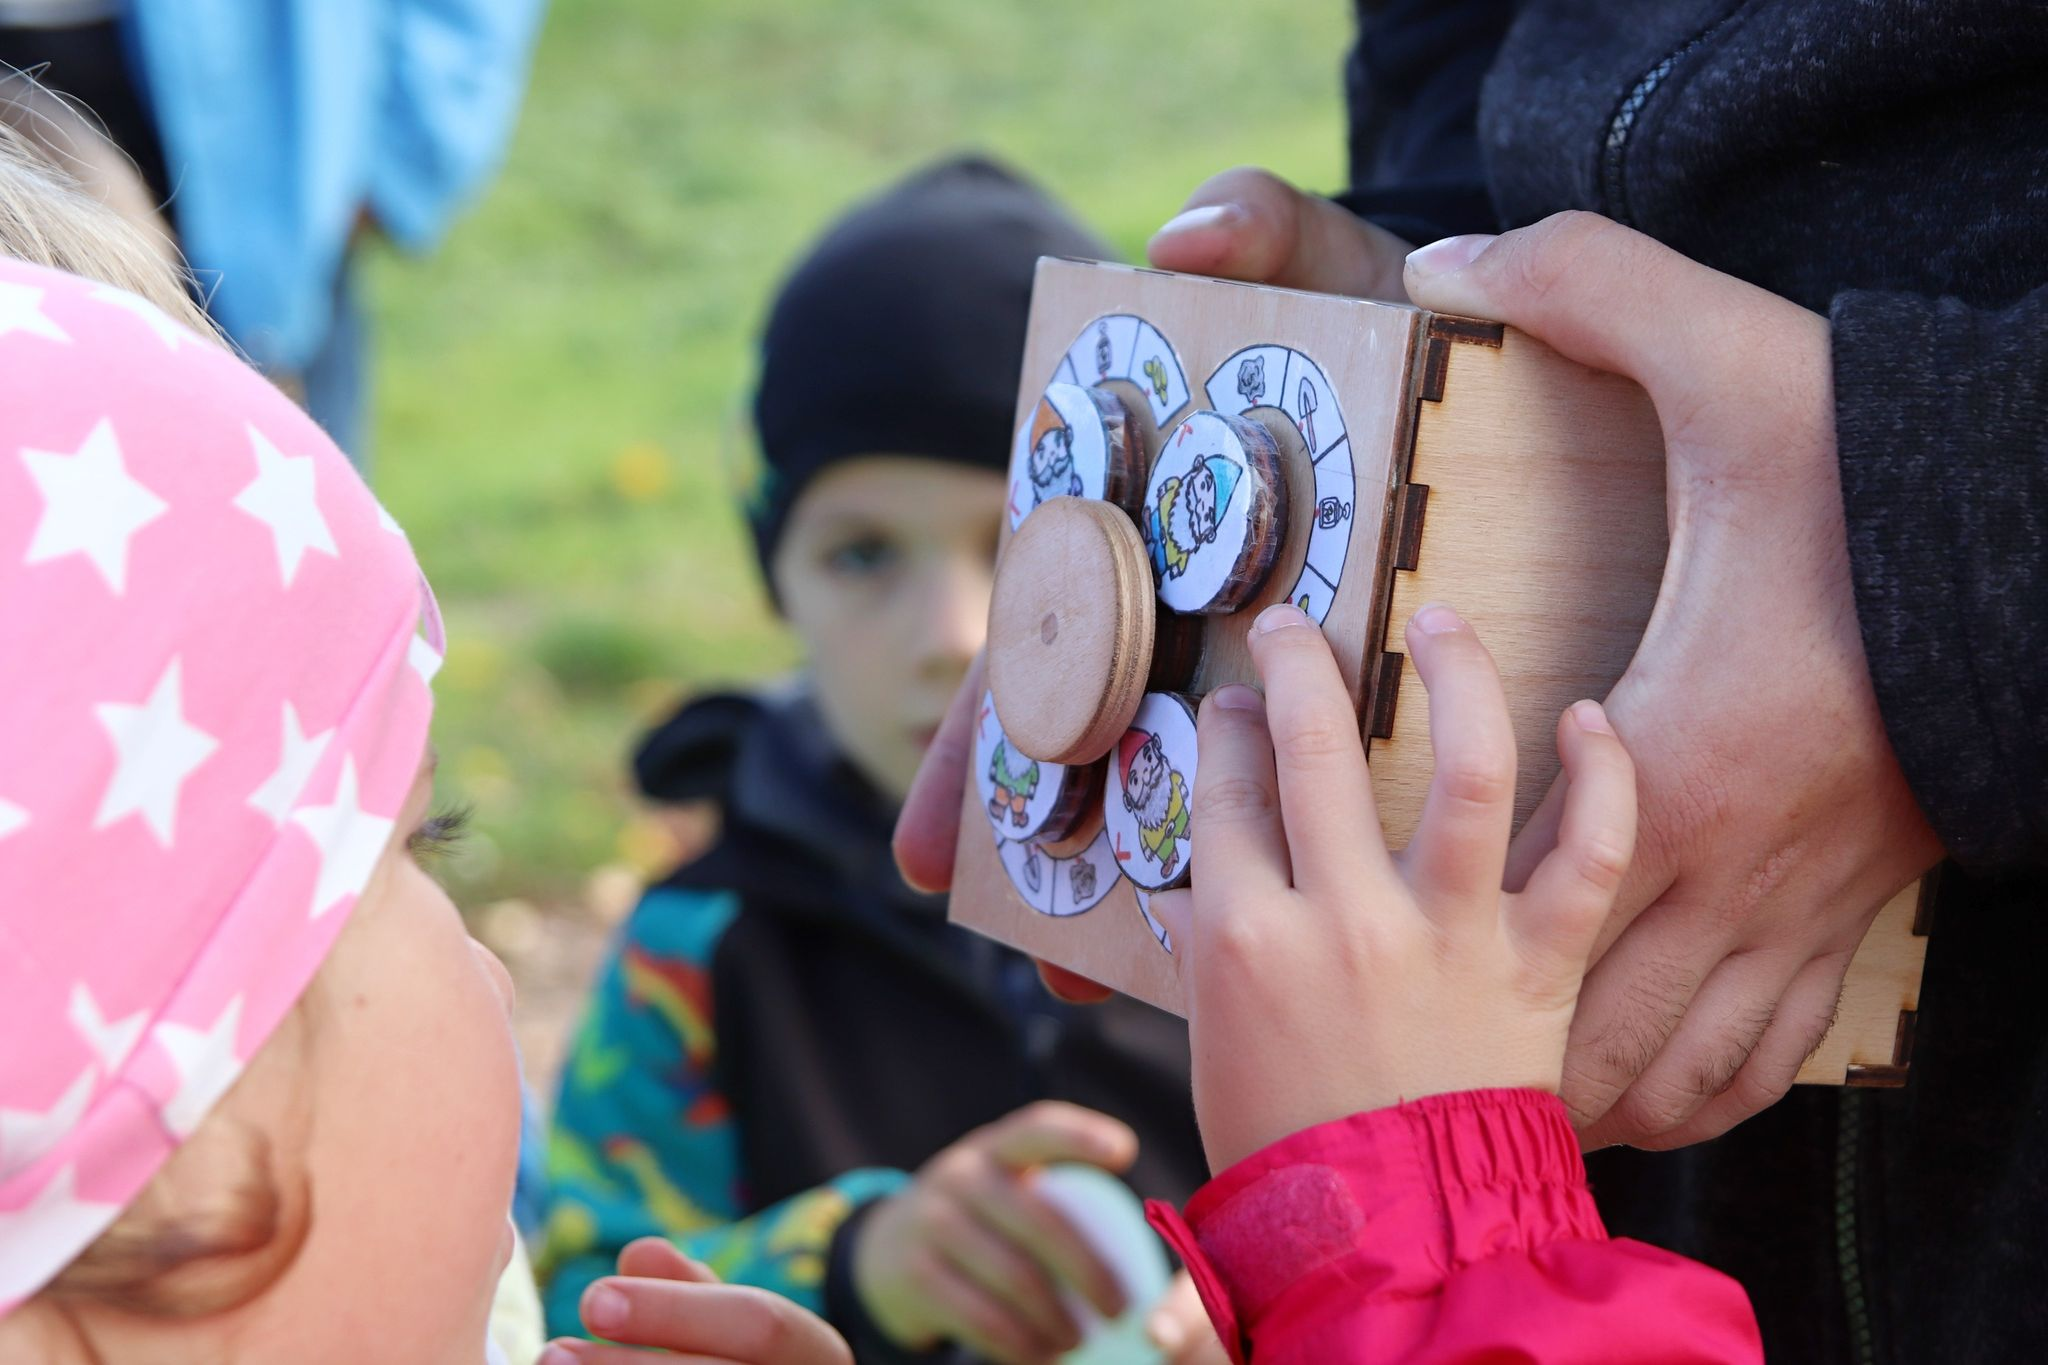
\includegraphics[width=\textwidth]{kapitoly/obrazky/M3/trpaslici.png}
    \caption{Trpasličí trezor}
    \label{fig:M3-trpaslici}
\end{figure}

%todo další akce nikdy moc nebyli v plánu, prostě se už počítalo s lockdownem takže se ani nic nevymýšlelo (bavil jsem se s Jirkou že mi vyrobí nějakej ten papír)

\chapter{Závěr}
Cílem mé práce bylo vyvinout systém v podobě trezoru pro výuku programování, mechanické stavby a náplň různých kolektivních her. 

Plánovaných cílů jsem dosáhl, přesto, že se v průběhu vývoje částečně změnil koncept celého systému. Trezor měl původně sloužit primárně pro výuku, ale v průběhu vývoje 
se objevilo daleko víc požadavků a možností na nasazení trezoru jako hotového zařízení např. v nejrůznějších táborových nebo městských hrách. 


% Kvůli pandemii a částečně i kvůli dosud probíhajícímu vývoji se těchto her ale dosud uskutečnilo velmi málo.

Díky teto práci jsem se zdokonalil v návrhu tištěních spojů. Také jsem pro návrh DPS začal využívat program KiCad, zatím dříve jsem využíval Eagle, který není špatný ale KiCad 
mi vyhovuje o něco více. Díky výrobě desek jsem se naučil používat program \href{https://github.com/yaqwsx/KiKit}{KiKit} \parencite{KiKit}, 
který vytvořil Jan Mrázek a který zásadně usnadňuje výrobu podkladu pro reálnou výrobu DPS.


%V závěru by mělo být:
%\begin{itemize}
%    \item Rekapitulace cíle práce
%    \item Dosáhnul jsem jej? Ano, nebo ne?
%    \item Zhodnocení průběhu práce             %totálně netuším co o tom napsat
%    \item Co mi práce dala?
%\end{itemize}


\appendix

%\noindent \huge \textbf{Obrazová příloha} \normalsize 

\newcommand\OdsazeniNadpisu{12mm}

\begin{figure}
    \appendix
    \chapter{Obrazová příloha}
	\section{Vzhled druhé elektronické varianty}
	\vspace{\OdsazeniNadpisu}
    \centering
    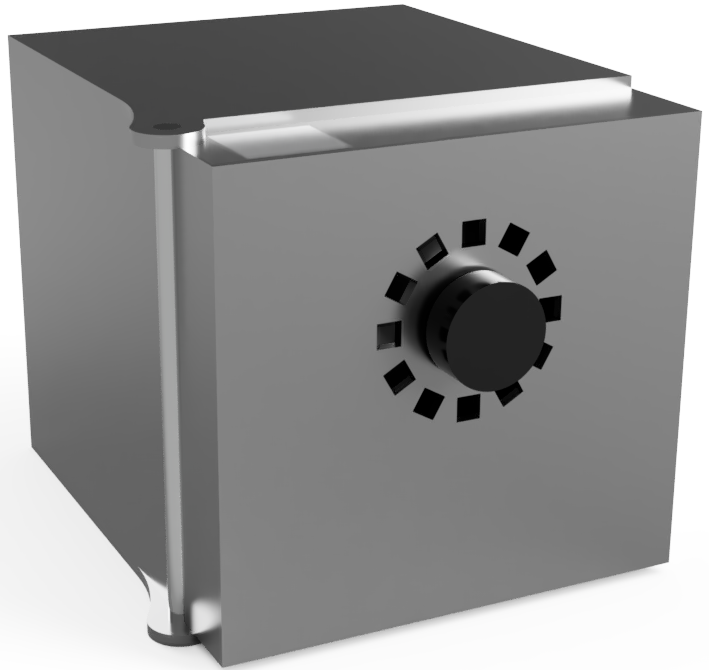
\includegraphics[width=0.7\textwidth]{kapitoly/obrazky/E2/predni_render.png}
    \caption{Render varianty E2}
    \label{fig:E2-render}
\end{figure}

\begin{figure}[htbp]
    \section{Vzhled třetí elektronické varianty}
	\centering
	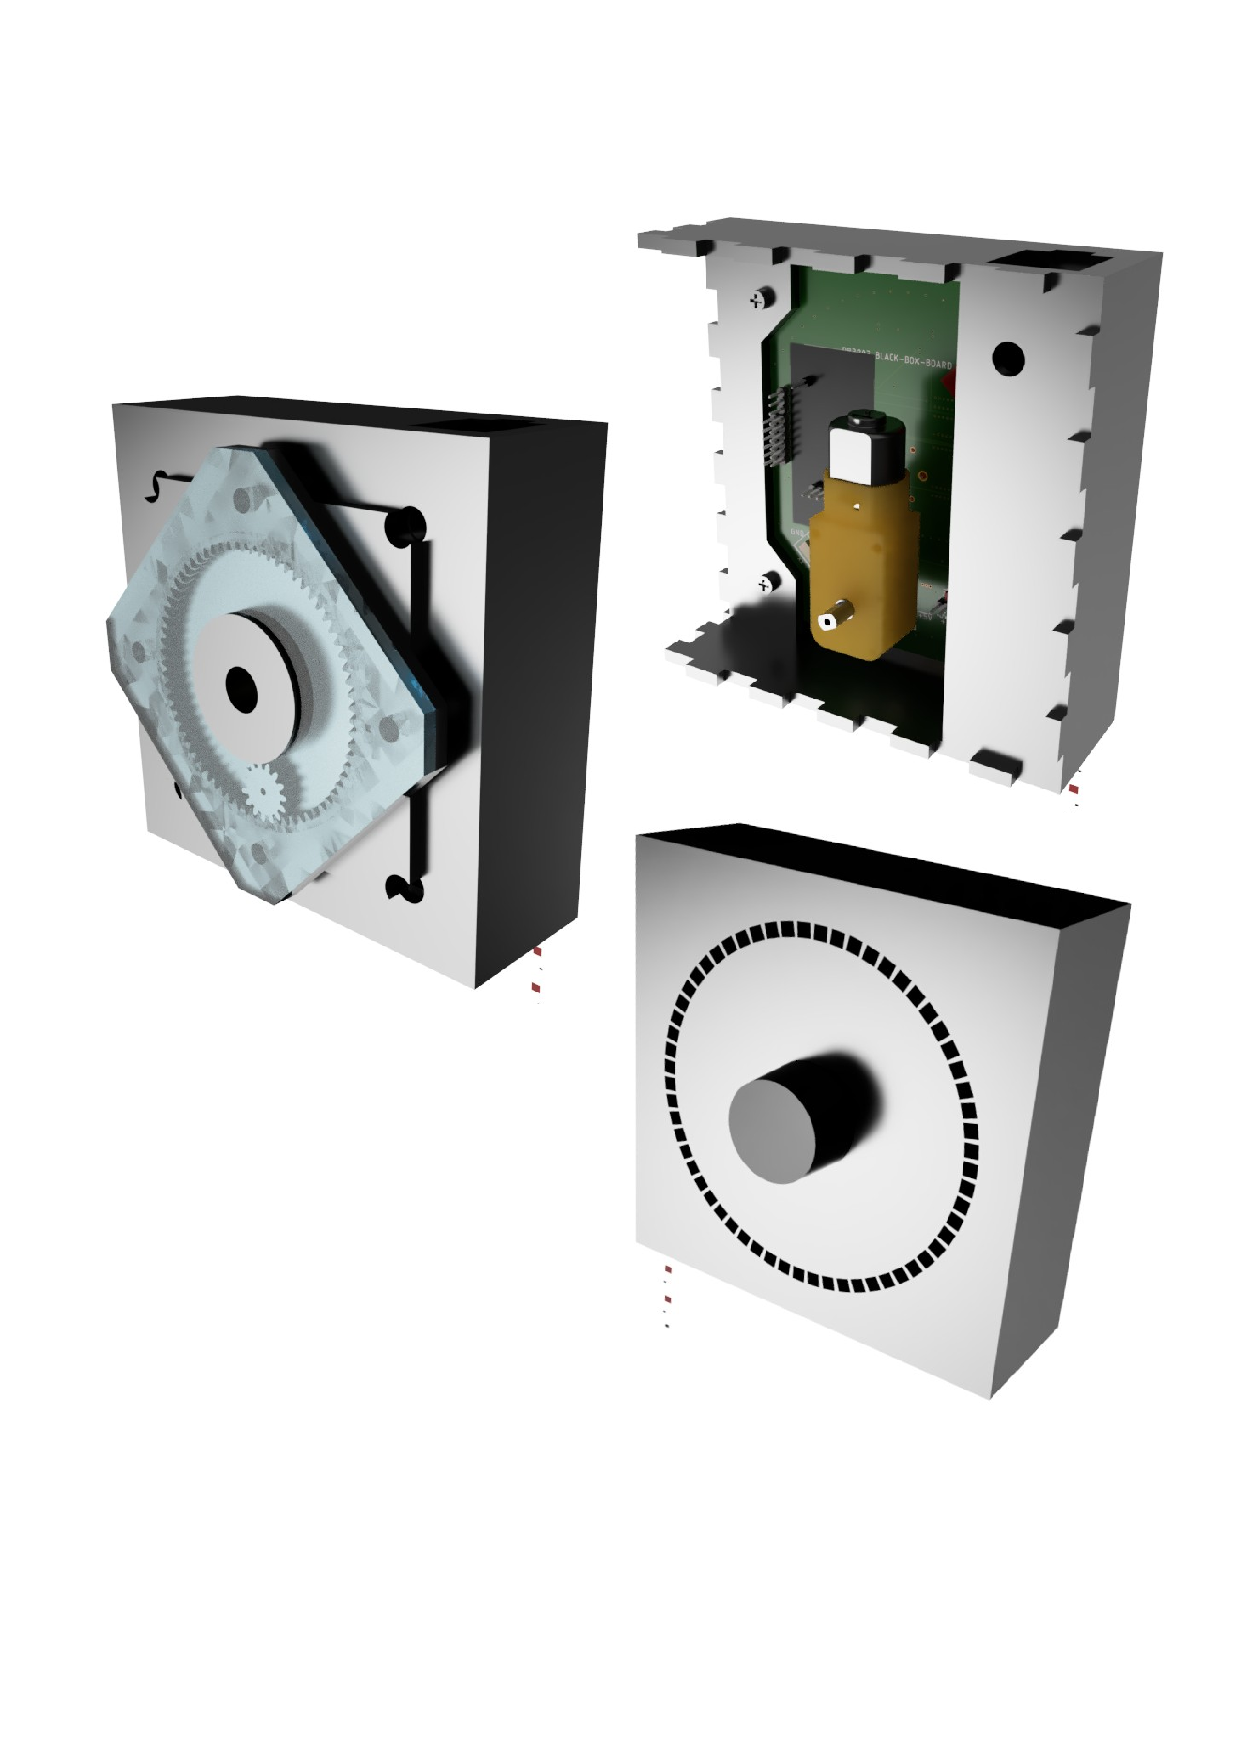
\includegraphics[width=\textwidth]{kapitoly/obrazky/E3/rendery.pdf}
	\caption{render varianty E3}
	\label{fig:E3-renderi}
\end{figure}

\begin{figure}
	\section{Vzhled druhé mechanické varianty}
	\vspace{\OdsazeniNadpisu}
    \centering
    \includegraphics[width=\textwidth]{kapitoly/obrazky/M2/predni_render.PNG}
    \caption{Render varianty M2}
    \label{fig:M2-render}
\end{figure}

\begin{figure}
    \section{Simulace pevnosti tlakové desky}
    \centering
    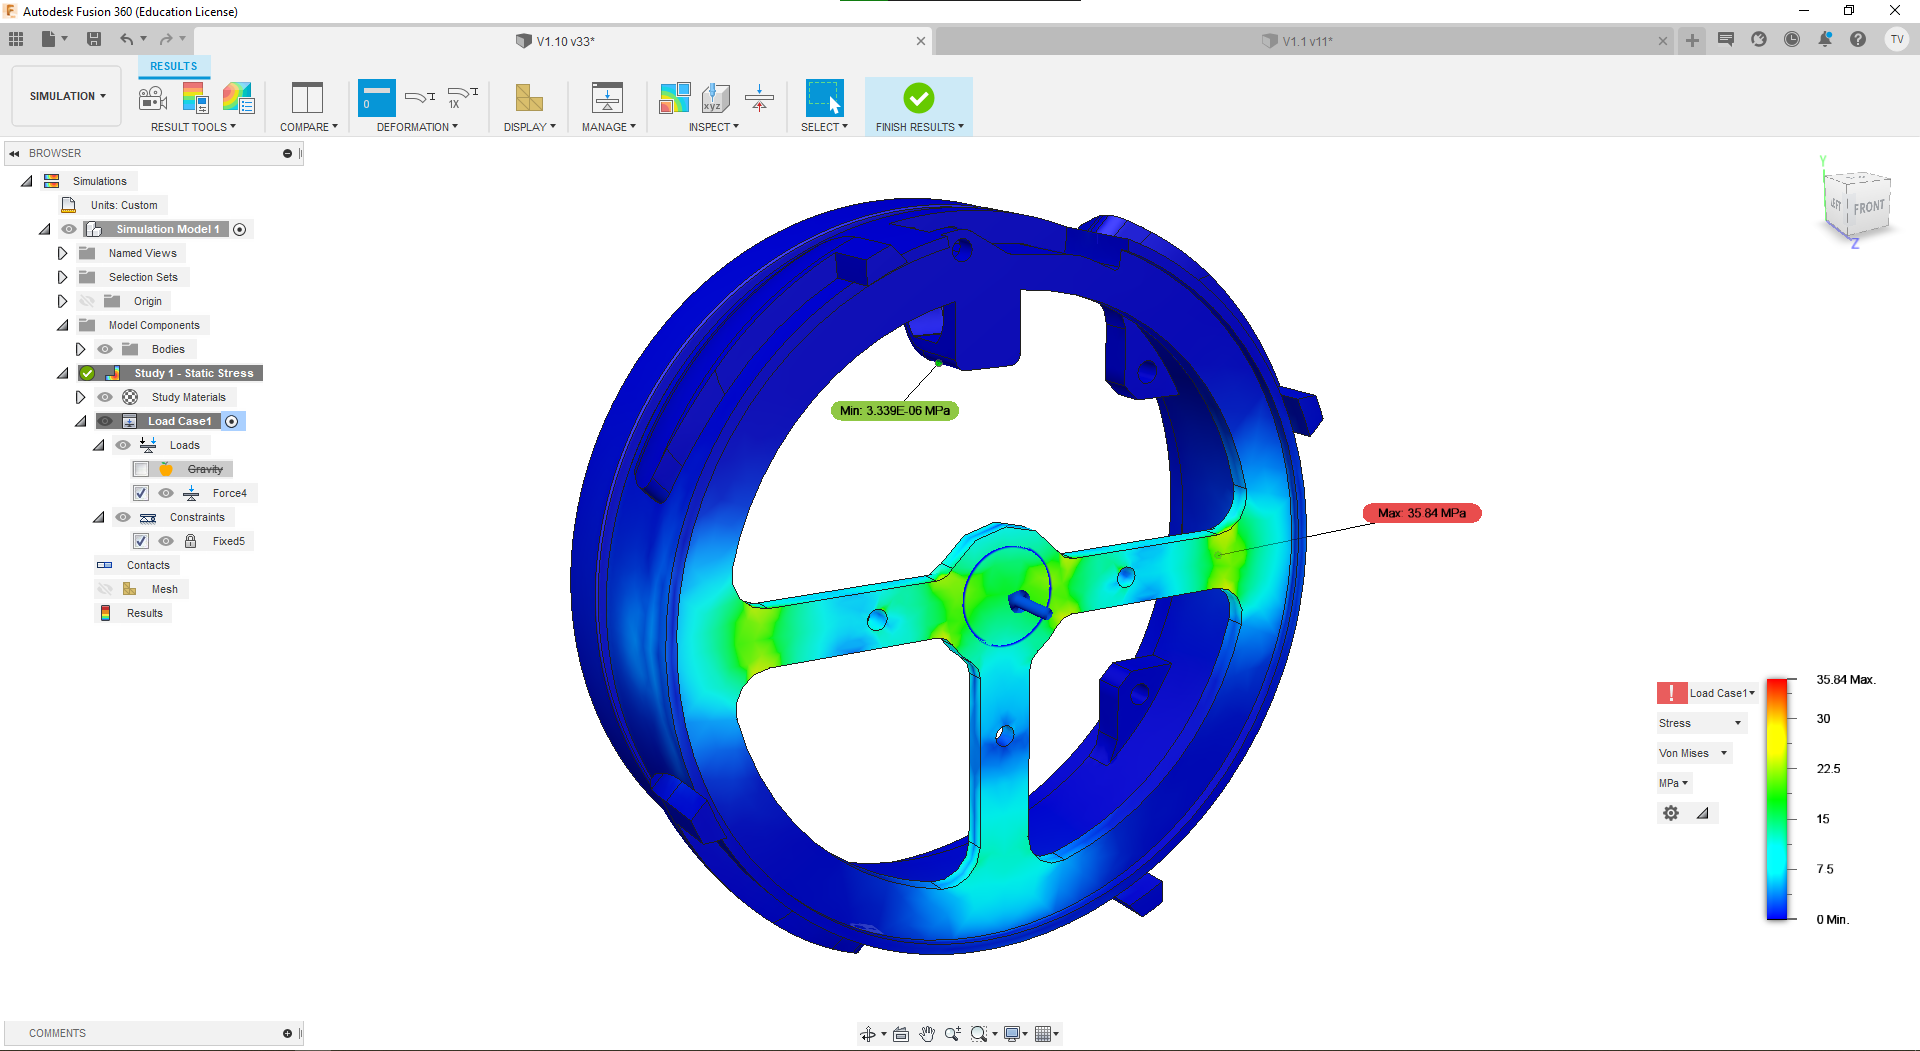
\includegraphics[width=370pt]{kapitoly/obrazky/E4/machanika_tlakove_desky/simulace/F100N,primo,uprostred,pohled_zepredu.png}
    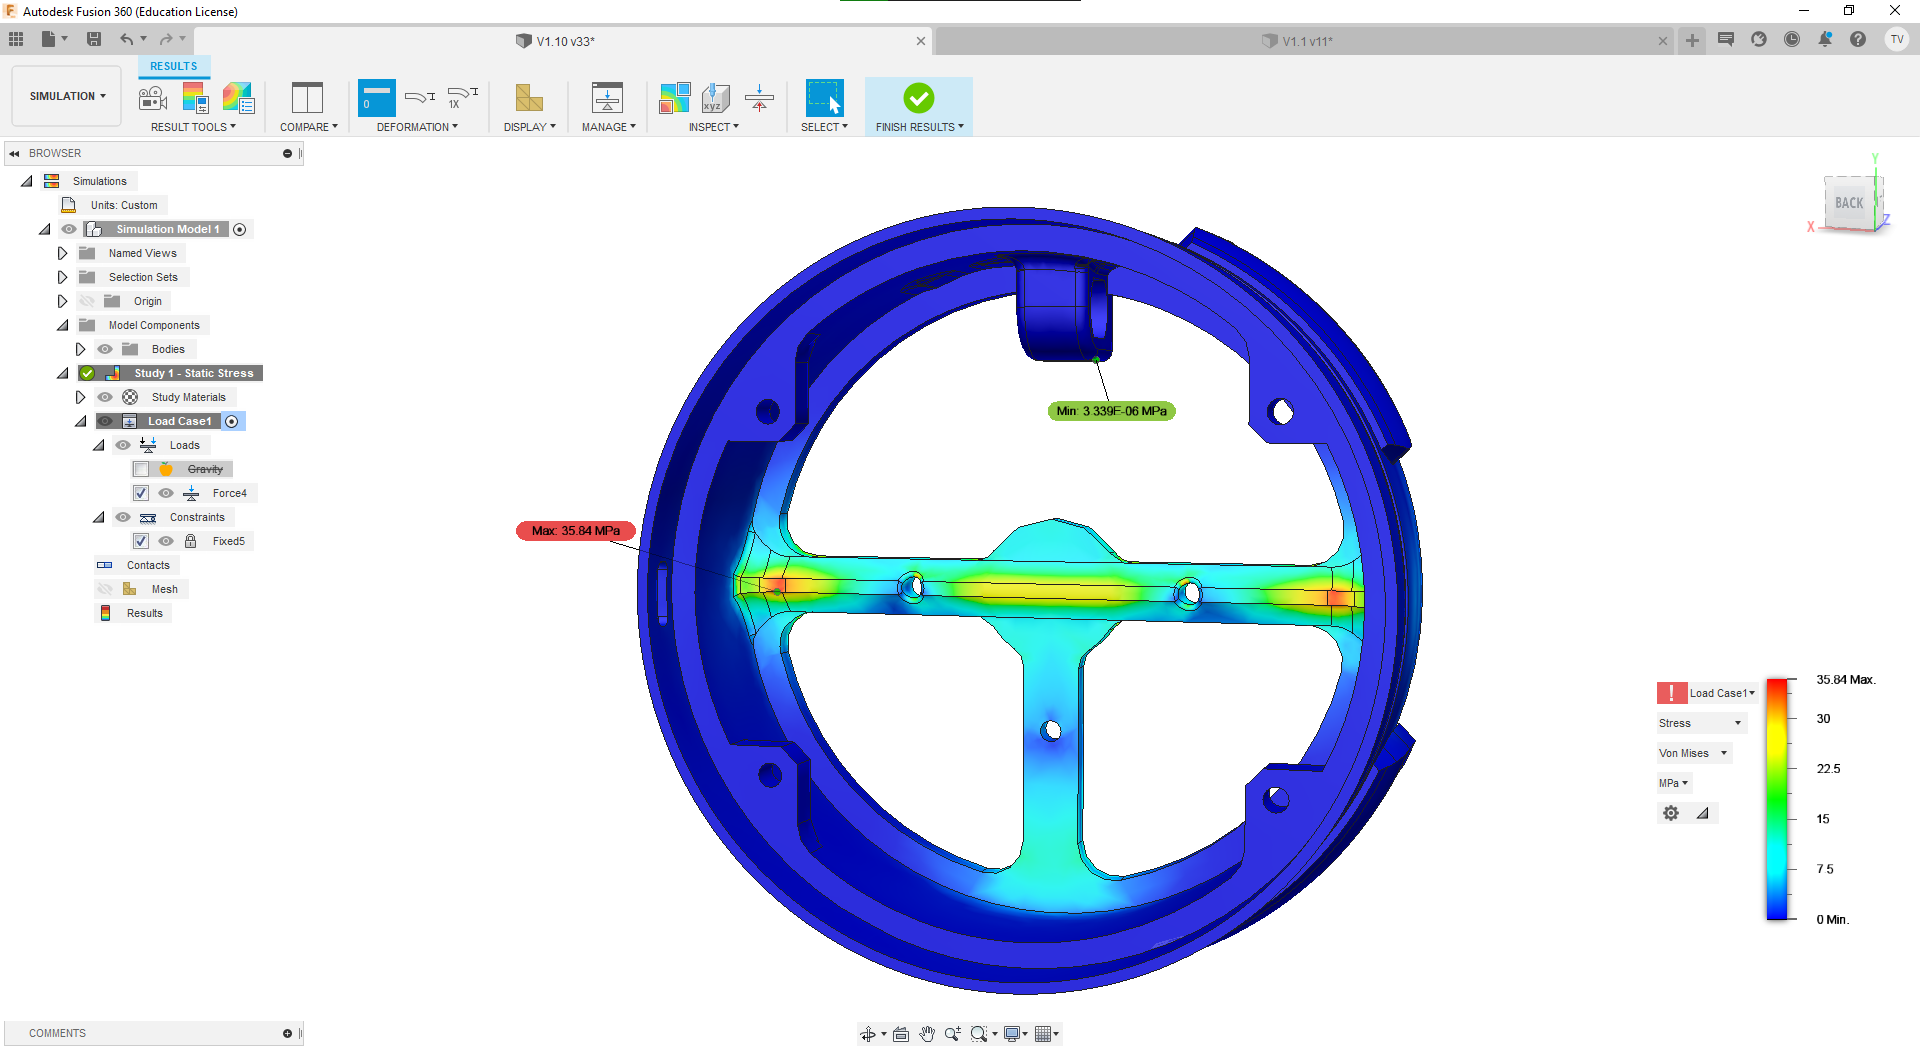
\includegraphics[width=370pt]{kapitoly/obrazky/E4/machanika_tlakove_desky/simulace/F100N,primo,uprostred,pohled_zezadu.png}
    \caption{Pevnostní simulace těla nahoře je pohled ze předu a dole pohled zezadu \centering}
    Tato simulace testuje působení síly přímo na tělo, což není působení, které by v provozu nastávalo. Takovéto namáhání je ale o dost náročnější
    než to, které by reálně nastalo.
    \label{fig:E4-simulace_tela} %todo těla čeho? trezor je hranatý? 
\end{figure}

\begin{figure}
    \centering
    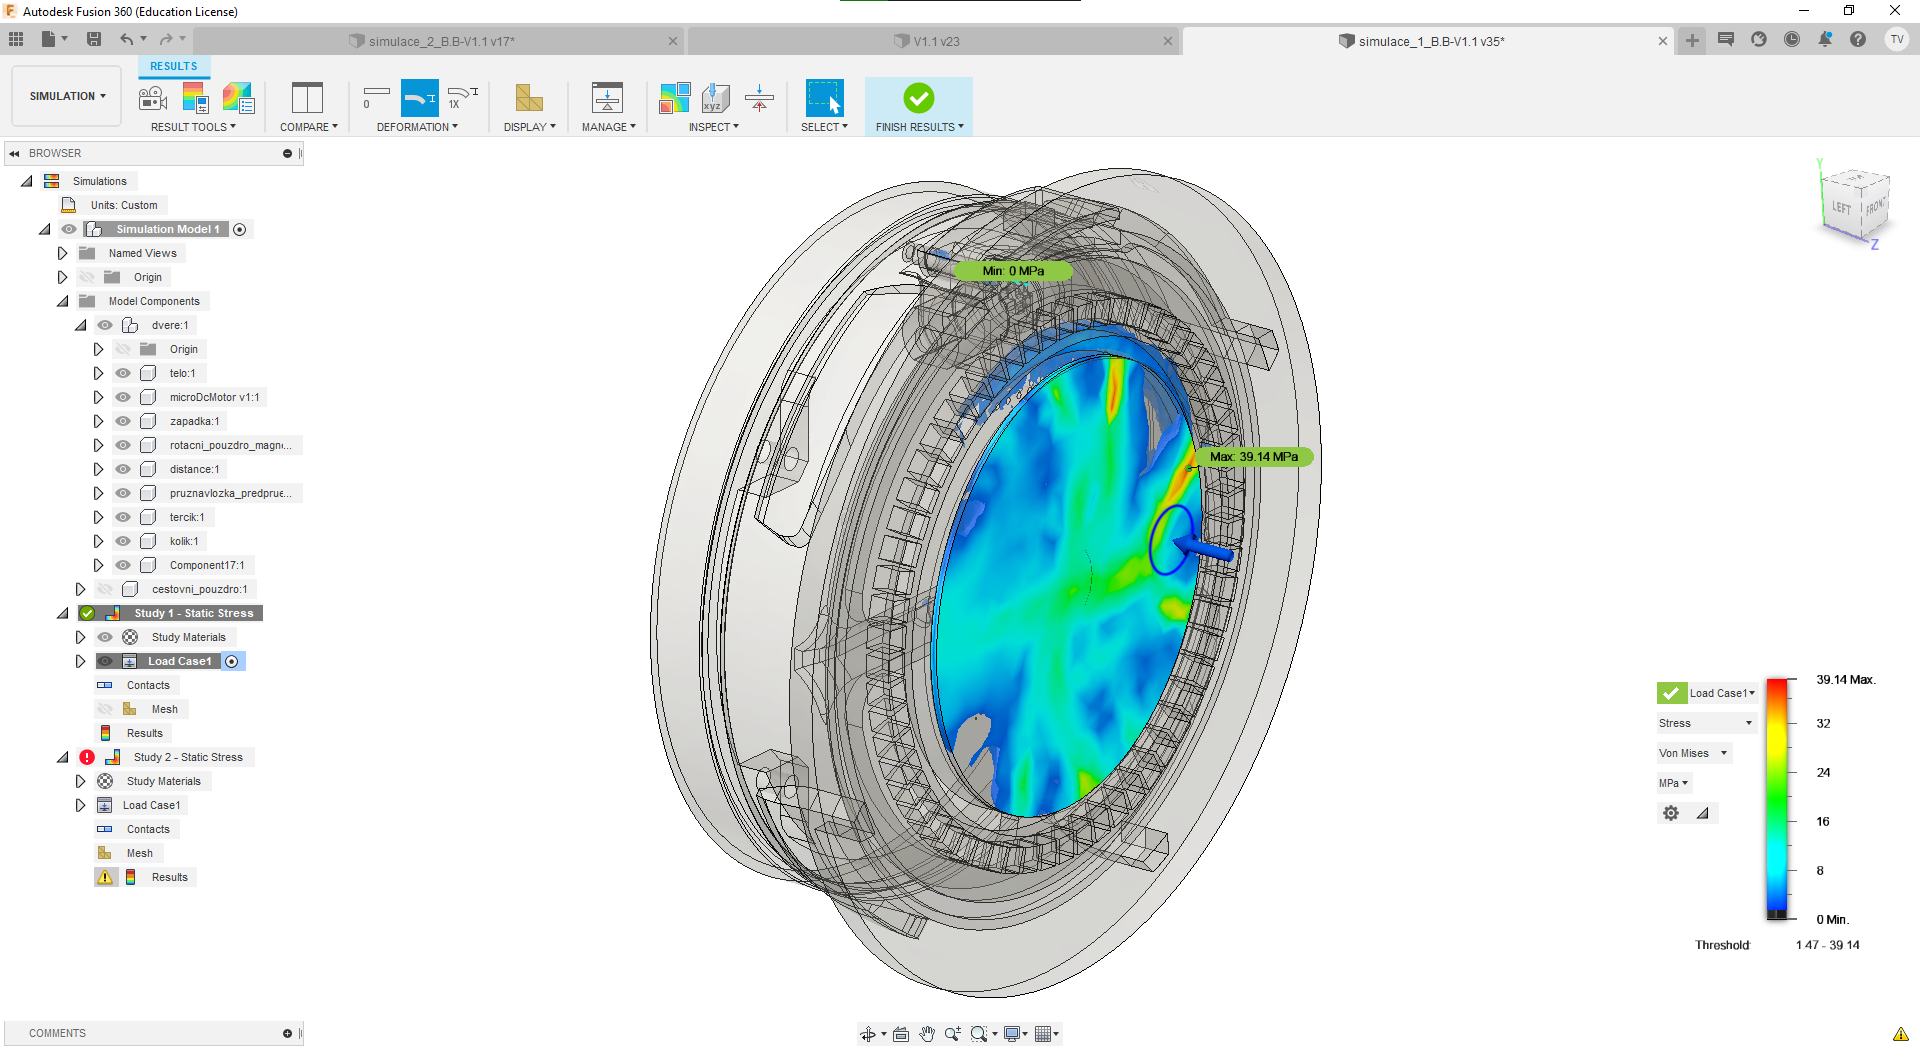
\includegraphics[width=\textwidth]{kapitoly/obrazky/E4/machanika_tlakove_desky/simulace/zjednodusena_sestava_pri_F100N_nezobrazeno_napeti_pod_1,5MPa.png}
    \caption{Simulace sestavy}
    Jak je vidět, tak i sílu 100~N dokaže sendvič z terčíku, pružné podložky a~snímací desky rozložit na dostatečnou plochu, aby napětí v těle nestouplo 
    nad cca 3~MPa. Na obrázku je zobrazené jen napětí nad 1,5~MPa.
    \label{fig:E4-simulace_tlakovky}
\end{figure}

\begin{figure}
    \section{Obrázky PCB}
    \centering
    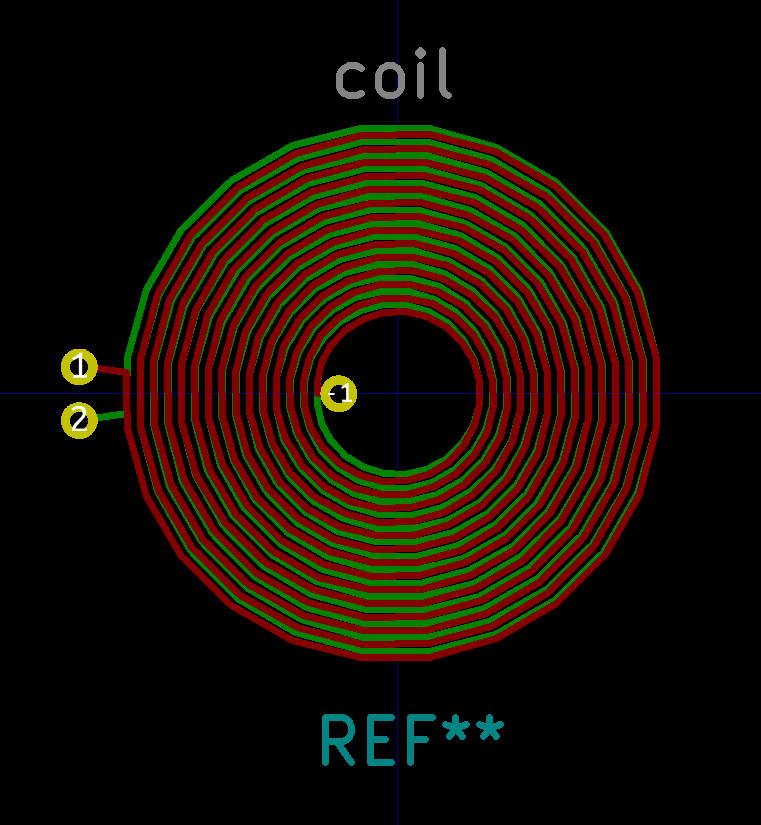
\includegraphics[width=\textwidth]{kapitoly/obrazky/E4/elektronika_tlakove_desky/civka.png}
    \caption{Vzhled reliéfu cívky}
    \label{fig:E4-relief_civka}
\end{figure}

\begin{figure}
    \centering
    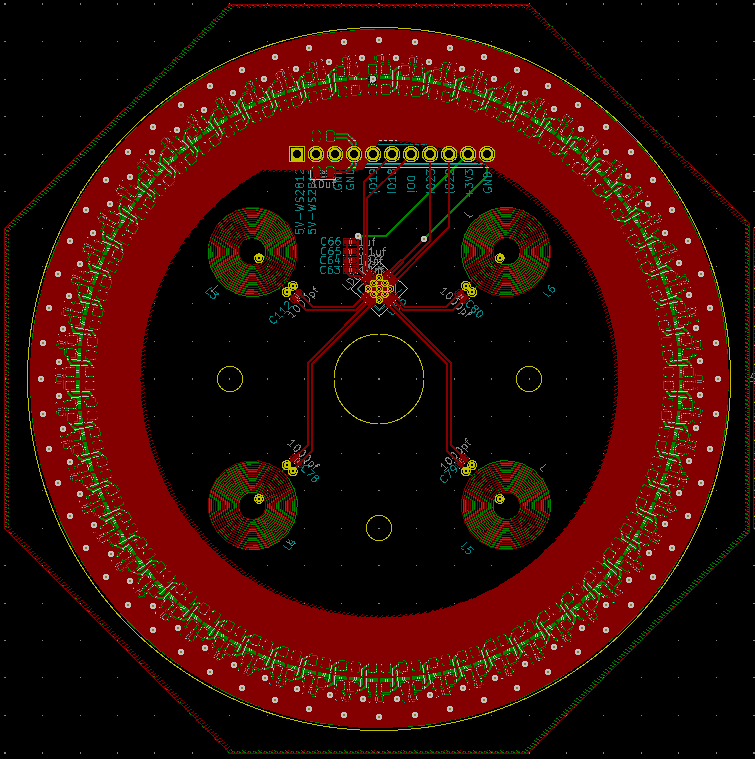
\includegraphics[width=\textwidth]{kapitoly/obrazky/E4/elektronika_tlakove_desky/leddeska-KiCad.png}
    \caption{Vzhled desky s kruhem WS2812 a snímáním tlakové desky}
    \label{fig:E4-LedDeska}
\end{figure}

\begin{figure}
    \section{Schémata}
    \centering
    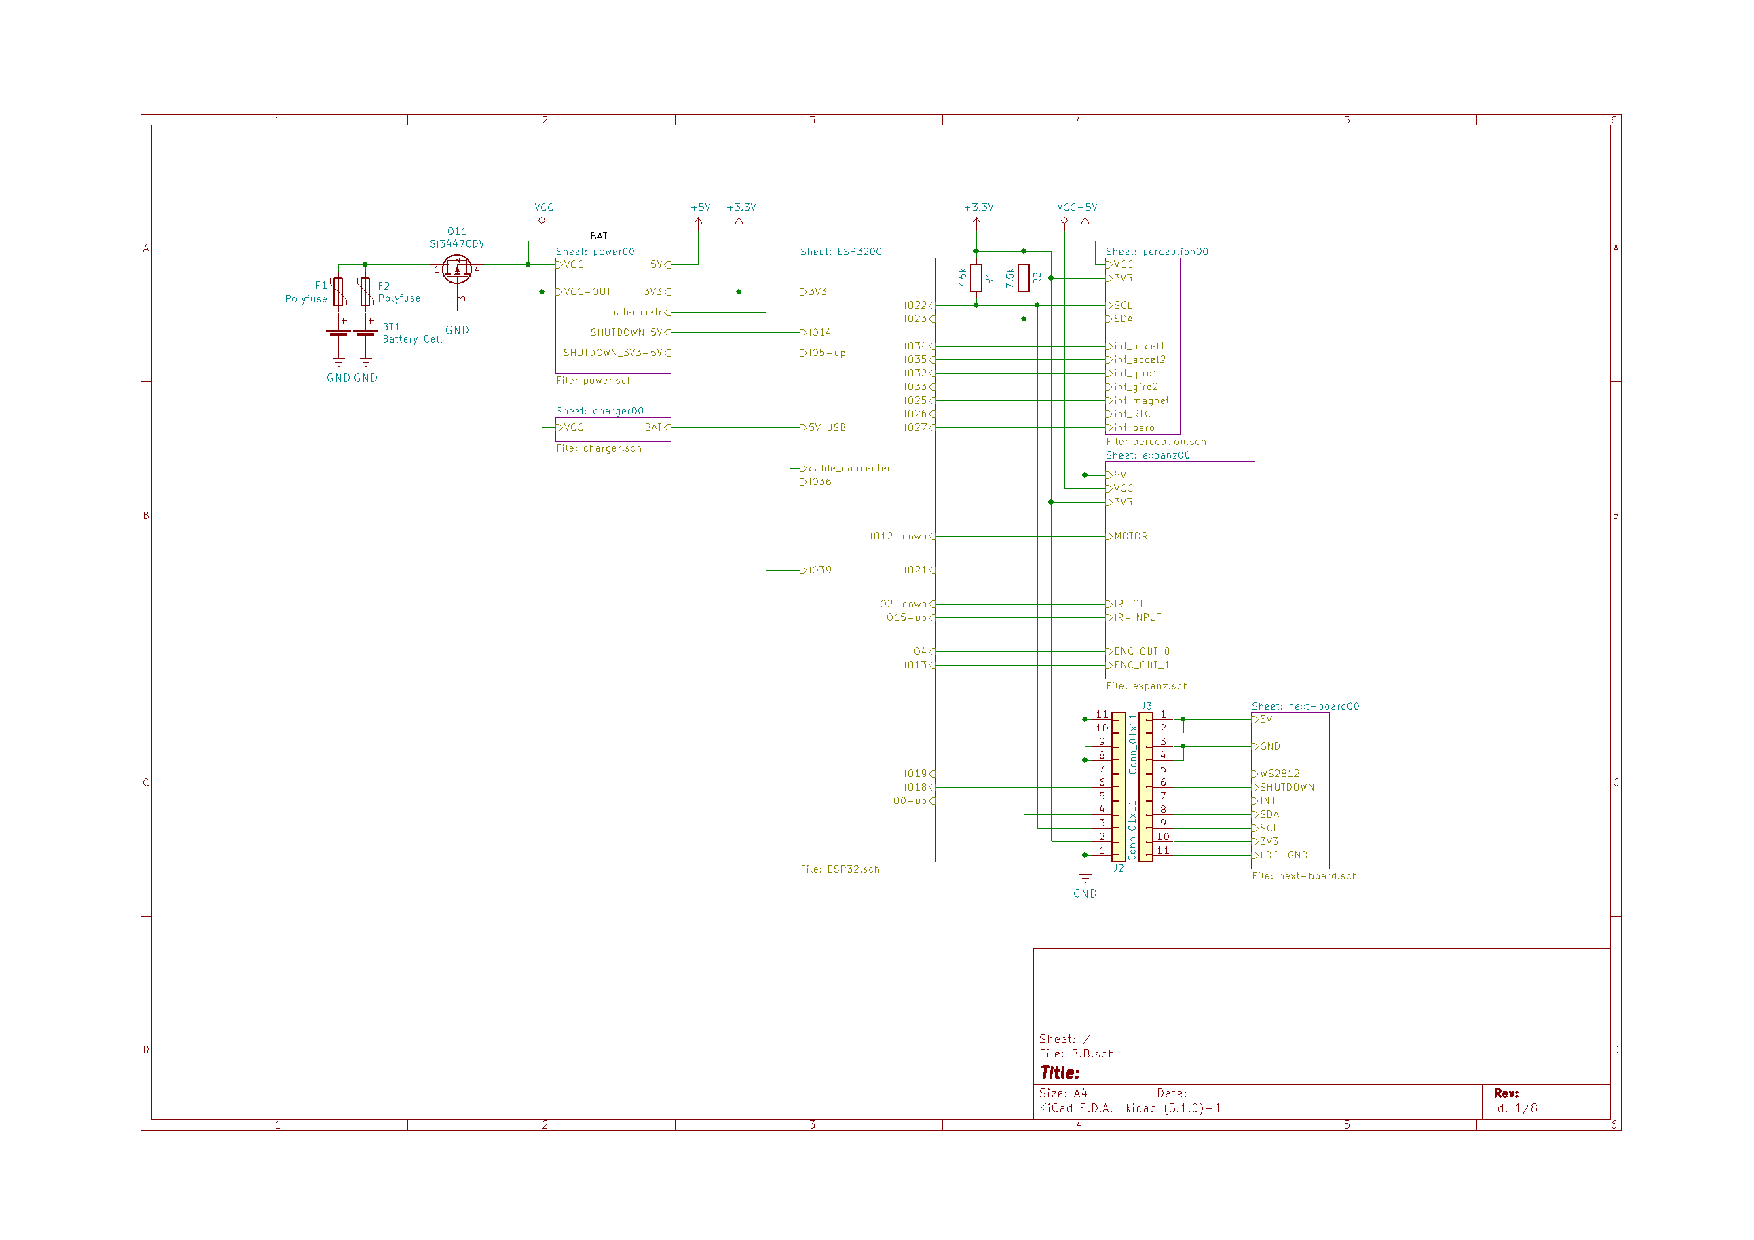
\includegraphics[width=0.93\textheight, angle=90]{kapitoly/ctvrta_elektronicka_varianta/E4_zapojeni/B.B.pdf}
    \caption{Propojení jednotlivých systémů -- schéma}
    \label{fig:E4-sch_B.B}
\end{figure}
\begin{figure}
    \centering
    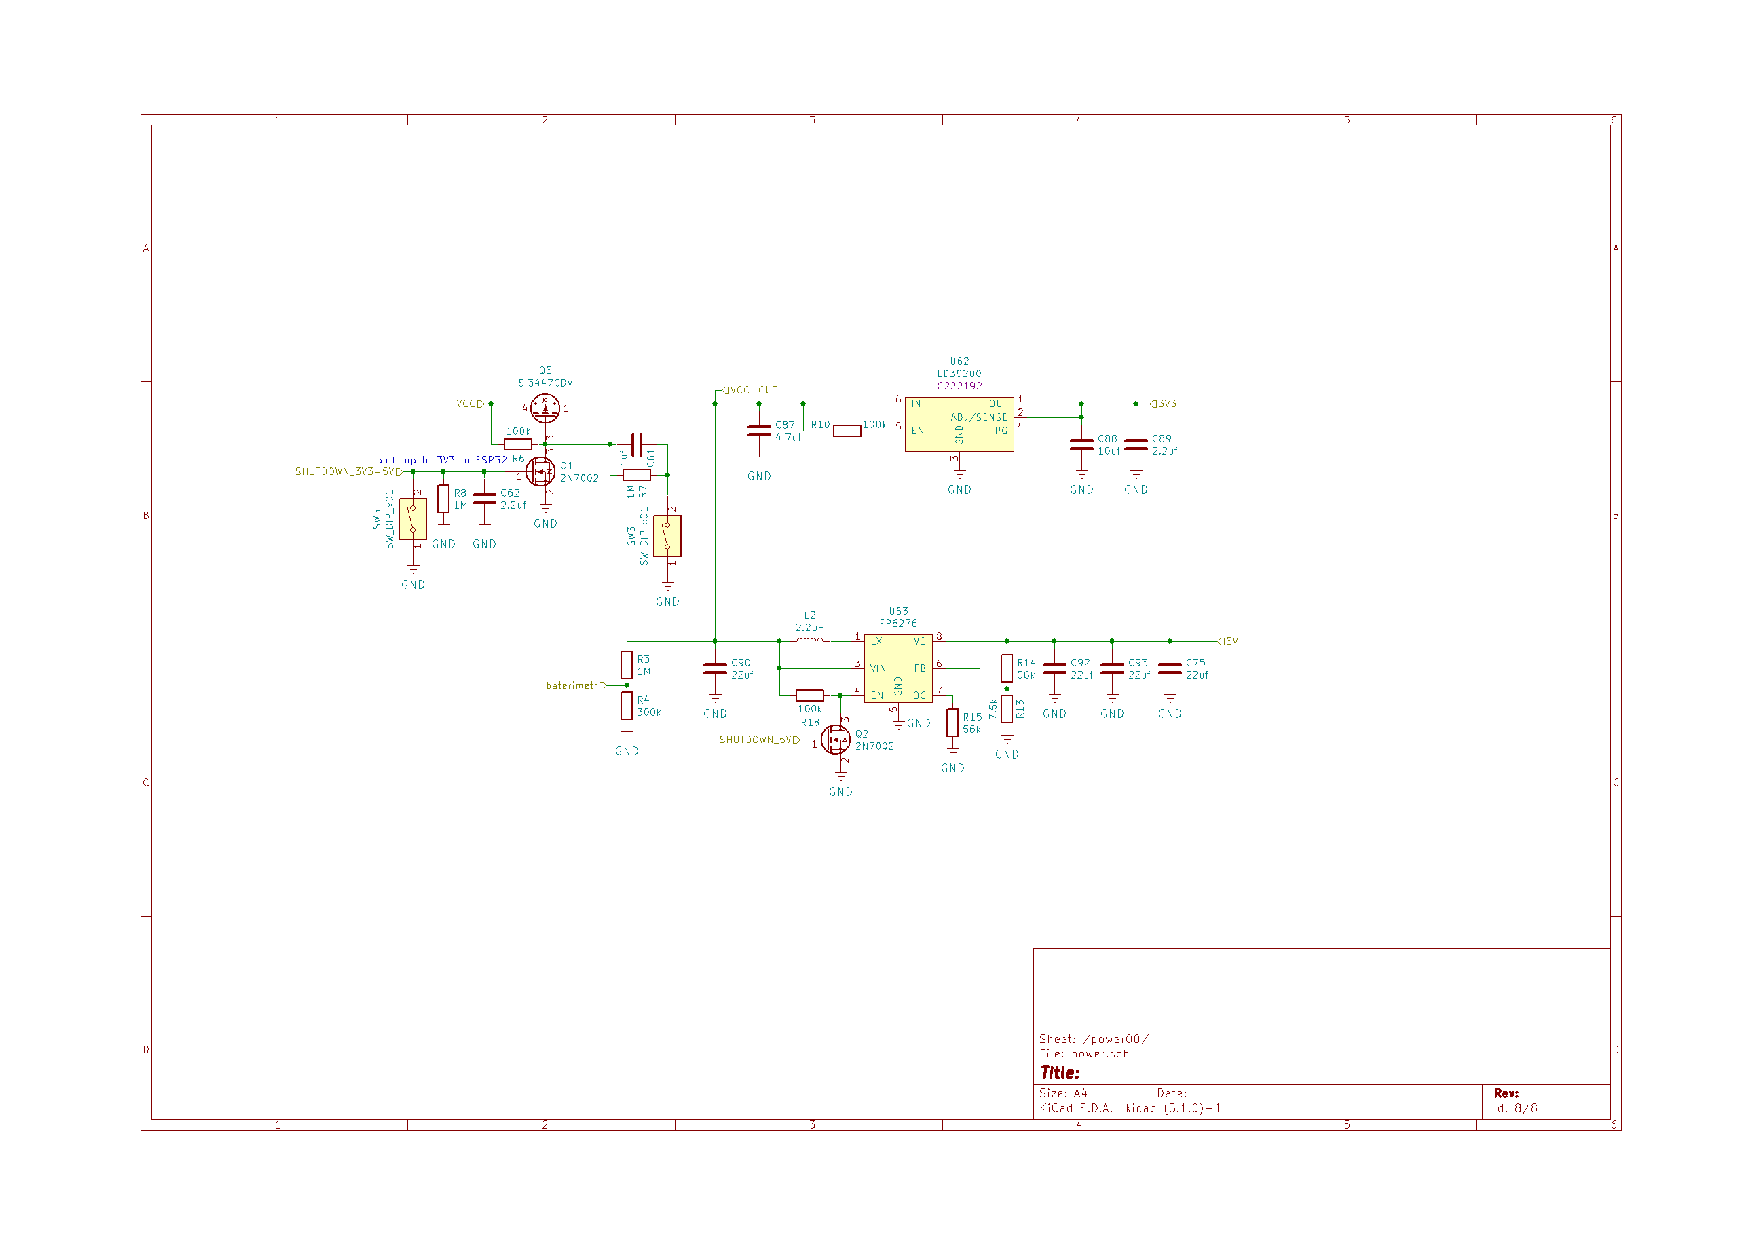
\includegraphics[width=0.93\textheight, angle=90]{kapitoly/ctvrta_elektronicka_varianta/E4_zapojeni/zdroj.pdf}
    \caption{Zapojení zdroje -- schéma}
    \label{fig:E4-sch_zdroj}
\end{figure}
\begin{figure}
    \centering
    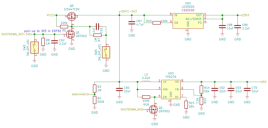
\includegraphics[width=0.93\textheight, angle=90]{kapitoly/ctvrta_elektronicka_varianta/E4_zapojeni/nabijecka.pdf}
    \caption{Zapojení nabíjecího obvodů -- schéma}
    \label{fig:E4-sch_nabijecka}
\end{figure}
\begin{figure}[htbp]
    \centering
    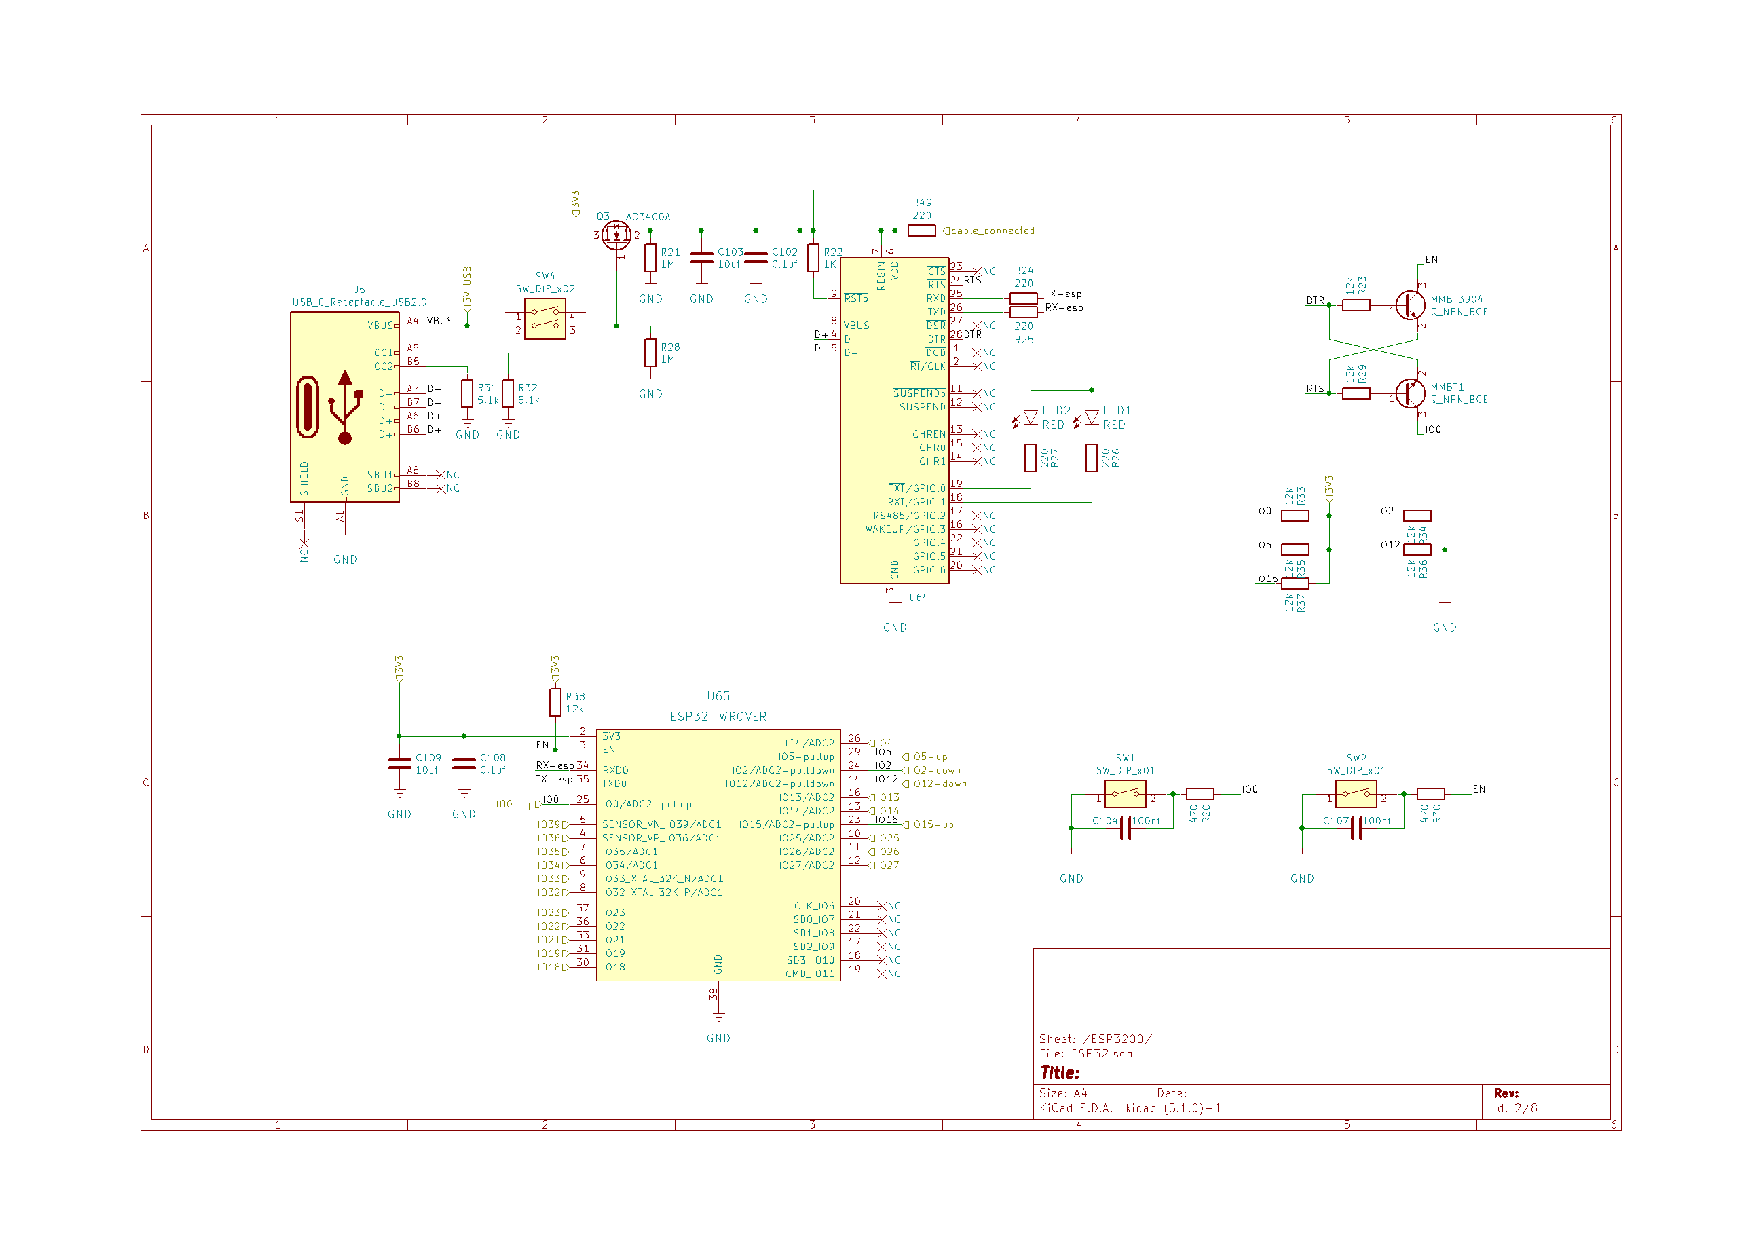
\includegraphics[width=0.93\textheight, angle=90]{kapitoly/ctvrta_elektronicka_varianta/E4_zapojeni/ESP32.pdf}
    \caption{Zapojení ESP32 a programátoru -- schéma}
    \label{fig:E4-sch_ESP32}
\end{figure}
\begin{figure}[htbp]
    \centering
    \includegraphics[width=0.93\textheight, angle=90]{kapitoly/ctvrta_elektronicka_varianta/E4_zapojeni/senzorika.pdf}
    \caption{Zapojení senzorů BMX055, MPU6050, QMC5883, M41T62, SPL06 a a konektoru pro A9G -- schéma \centering}
    \label{fig:E4-sch_senzorika}
\end{figure}
\begin{figure}[htbp]
    \centering
    \includegraphics[width=0.93\textheight, angle=90]{kapitoly/ctvrta_elektronicka_varianta/E4_zapojeni/IR_motor_enkoder.pdf}
    \caption{Zapojení IR komunikace, motoru a enkodéru -- schéma}
    \label{fig:E4-sch_IR-Motor-enkoder}
\end{figure}
\begin{figure}[htbp]
    \centering
    \includegraphics[width=0.93\textheight, angle=90]{kapitoly/ctvrta_elektronicka_varianta/E4_zapojeni/next_board.pdf}
    \caption{Zapojení LDC1614 -- schéma}
    \label{fig:E4-sch_next-board}
\end{figure}
\begin{figure}[htbp]
    \centering
    \includegraphics[width=0.93\textheight, angle=90]{kapitoly/ctvrta_elektronicka_varianta/E4_zapojeni/WS2812.pdf}
    \caption{Zapojení LED WS2812 na desce trezoru -- schéma}
    \label{fig:E4-sch_WS2812}
\end{figure}

\chapter{Ostatní přílohy}
\addtocounter{section}{1}
\addcontentsline{toc}{section}{\protect\numberline{\thesection}Seznam obrázků} 
\listoffigures

\addtocounter{section}{1}
\addcontentsline{toc}{section}{\protect\numberline{\thesection}Literatura}
\printbibheading 
\printbibliography[keyword=datasheeth,heading=subbibliography,title={Technická dokumentace}]
\printbibliography[keyword=online,heading=subbibliography,title={Ostatní internetové zdroje}]

\addtocounter{section}{1}
\addcontentsline{toc}{section}{\protect\numberline{\thesection}Seznam tabulek}
\listoftables

\end{document}

%todo ověřit číslování stránek práce
